% **************************************************************************************************************
% A Classic Thesis Style
% An Homage to The Elements of Typographic Style
%
% Copyright (C) 2018 André Miede and Ivo Pletikosić
%
% If you like the style then I would appreciate a postcard. My address
% can be found in the file ClassicThesis.pdf. A collection of the
% postcards I received so far is available online at
% http://postcards.miede.de
%
% License:
% This program is free software; you can redistribute it and/or modify
% it under the terms of the GNU General Public License as published by
% the Free Software Foundation; either version 2 of the License, or
% (at your option) any later version.
%
% This program is distributed in the hope that it will be useful,
% but WITHOUT ANY WARRANTY; without even the implied warranty of
% MERCHANTABILITY or FITNESS FOR A PARTICULAR PURPOSE.  See the
% GNU General Public License for more details.
%
% You should have received a copy of the GNU General Public License
% along with this program; see the file COPYING.  If not, write to
% the Free Software Foundation, Inc., 59 Temple Place - Suite 330,
% Boston, MA 02111-1307, USA.
%
% PLEASE SEE ALSO THE AUTHORS' NOTE REGARDING THIS LICENSE
% IN THE DOCUMENTATION (ClassicThesis.pdf --> Chapter 1 / Chapter01.tex)
% **************************************************************************************************************
\RequirePackage{silence} % :-\
    \WarningFilter{scrreprt}{Usage of package `titlesec'}
    %\WarningFilter{scrreprt}{Activating an ugly workaround}
    \WarningFilter{titlesec}{Non standard sectioning command detected}
\documentclass[ twoside,openright,titlepage,numbers=noenddot,%1headlines,
                headinclude,footinclude,cleardoublepage=empty,abstract=on,
                BCOR=5mm,paper=a4,fontsize=10pt
                ]{scrreprt}

%********************************************************************
% Note: Make all your adjustments in here
%*******************************************************
% ****************************************************************************************************
% classicthesis-config.tex
% formerly known as loadpackages.sty, classicthesis-ldpkg.sty, and classicthesis-preamble.sty
% Use it at the beginning of your ClassicThesis.tex, or as a LaTeX Preamble
% in your ClassicThesis.{tex,lyx} with % ****************************************************************************************************
% classicthesis-config.tex
% formerly known as loadpackages.sty, classicthesis-ldpkg.sty, and classicthesis-preamble.sty
% Use it at the beginning of your ClassicThesis.tex, or as a LaTeX Preamble
% in your ClassicThesis.{tex,lyx} with % ****************************************************************************************************
% classicthesis-config.tex
% formerly known as loadpackages.sty, classicthesis-ldpkg.sty, and classicthesis-preamble.sty
% Use it at the beginning of your ClassicThesis.tex, or as a LaTeX Preamble
% in your ClassicThesis.{tex,lyx} with \input{classicthesis-config}
% ****************************************************************************************************
% If you like the classicthesis, then I would appreciate a postcard.
% My address can be found in the file ClassicThesis.pdf. A collection
% of the postcards I received so far is available online at
% http://postcards.miede.de
% ****************************************************************************************************


% ****************************************************************************************************
% 0. Set the encoding of your files. UTF-8 is the only sensible encoding nowadays. If you can't read
% äöüßáéçèê∂åëæƒÏ€ then change the encoding setting in your editor, not the line below. If your editor
% does not support utf8 use another editor!
% ****************************************************************************************************
\PassOptionsToPackage{utf8}{inputenc}
  \usepackage{inputenc}

\PassOptionsToPackage{T1}{fontenc} % T2A for cyrillics
  \usepackage{fontenc}


% ****************************************************************************************************
% 1. Configure classicthesis for your needs here, e.g., remove "drafting" below
% in order to deactivate the time-stamp on the pages
% (see ClassicThesis.pdf for more information):
% ****************************************************************************************************
\PassOptionsToPackage{
  drafting=false,    % print version information on the bottom of the pages
  tocaligned=false, % the left column of the toc will be aligned (no indentation)
  dottedtoc=true,  % page numbers in ToC flushed right
  parts,
  eulerchapternumbers=true, % use AMS Euler for chapter font (otherwise Palatino)
  linedheaders=false,       % chaper headers will have line above and beneath
  floatperchapter=true,     % numbering per chapter for all floats (i.e., Figure 1.1)
  eulermath=true,  % use awesome Euler fonts for mathematical formulae (only with pdfLaTeX)
  beramono=true,    % toggle a nice monospaced font (w/ bold)
  subfig,
  palatino=true,    % deactivate standard font for loading another one, see the last section at the end of this file for suggestions
  style=classicthesis % classicthesis, arsclassica
}{classicthesis}


% ****************************************************************************************************
% 2. Personal data and user ad-hoc commands (insert your own data here)
% ****************************************************************************************************
\newcommand{\myTitle}{Deep Learning Methods for Clinical Sleep Analysis\xspace}
\newcommand{\mySubtitle}{An Exploration in Computational Sleep Science}
\newcommand{\myDegree}{Doctor of Philosophy (PhD)\xspace}
\newcommand{\myDocument}{PhD Thesis\xspace}
\newcommand{\myName}{Alexander Neergaard Olesen\xspace}
\newcommand{\myProf}{Associate Professor MSK, Helge. B. D. Sørensen, PhD, MSc. E.E.\xspace}
\newcommand{\myOtherProf}{Professor Poul Jennum, MD, PhD\xspace}
\newcommand{\mySupervisor}{Professor Emmanuel Mignot, MD, PhD\xspace}
\newcommand{\myFaculty}{Department of Health Technology\xspace}
\newcommand{\myDepartment}{Section for Digital Health\xspace}
\newcommand{\myUni}{Technical University of Denmark\xspace}
\newcommand{\myLocation}{Kgs. Lyngby\xspace}
\newcommand{\myTime}{April 2020\xspace}
\newcommand{\myVersion}{\classicthesis}
\newcommand{\myAddress}{Ørsteds Plads\\Building 345C\\DK-2800 \myLocation\\Denmark}

% ********************************************************************
% Setup, finetuning, and useful commands
% ********************************************************************
\providecommand{\mLyX}{L\kern-.1667em\lower.25em\hbox{Y}\kern-.125emX\@}
\newcommand{\ie}{i.\,e.\xspace}
\newcommand{\Ie}{I.\,e.\xspace}
\newcommand{\eg}{e.\,g.\xspace}
\newcommand{\Eg}{E.\,g.\xspace}
\newcommand{\etc}{\textit{etc.\xspace}}
\newcommand{\etal}{\textit{et al.}\xspace}
% \newcommand{\cohen}{Cohen's $\kappa$}
\newcommand{\wake}{\textsc{w}\xspace}
\newcommand{\rem}{\textsc{r}\xspace}
\newcommand{\nrem}{\textsc{nrem}\xspace}
\newcommand{\nI}{\textsc{n1}\xspace}
\newcommand{\nII}{\textsc{n2}\xspace}
\newcommand{\nIII}{\textsc{n3}\xspace}
\newcommand{\ntI}{\textsc{nt1}\xspace}
\newcommand{\real}[1]{\mathbb{R}^{#1}\xspace}
\newcommand{\cohen}{Cohen's~\ensuremath{\kappa}\xspace}
\newcommand{\ci}[4]{\ensuremath{#1 \pm #2}, \SI{95}{\percent} CI: \ensuremath{\left[ #3-#4 \right]}\xspace}
\newcommand{\muci}[3]{#1 (\SI{95}{\percent} CI: \ensuremath{\left[ #2-#3 \right])}\xspace}
\newcommand{\meanstdrange}[4]{\num[separate-uncertainty]{#1 +- #2} \ensuremath{\left[#3-#4 \right]}\xspace}
\newcommand{\plusminus}[2]{\num[separate-uncertainty]{#1+-#2}}
\newcommand{\train}{\textsc{train}\xspace}
\newcommand{\eval}{\textsc{eval}\xspace}
\newcommand{\test}{\textsc{test}\xspace}
\newcommand{\eog}{\textsc{eog}\xspace}
\newcommand{\mbl}{\mathcal{M}_{\mathrm{FM}}\xspace}
\newcommand{\mpt}{\mathcal{M}_{\mathrm{PT}}\xspace}
\newcommand{\mft}{\mathcal{M}_{\mathrm{FT}}\xspace}
\newcommand{\mse}{\mathcal{M}_{\mathrm{SE}}\xspace}
\newcommand{\N}{\mathbb{N}\xspace}
\newcommand{\hla}{\textsc{hla-dqb1*06:02}\xspace}
\newcommand{\oned}{\textsc{1d}\xspace}
\newcommand{\twod}{\textsc{2d}\xspace}
\newcommand{\threed}{\textsc{3d}\xspace}
\newcommand{\describe}[1]{\acs{#1}:~\acl{#1}}
\newcommand{\R}[1]{\mathbb{R}^{#1}\xspace}
% ****************************************************************************************************


% ****************************************************************************************************
% 3. Loading some handy packages
% ****************************************************************************************************
% ********************************************************************
% Packages with options that might require adjustments
% ********************************************************************
\PassOptionsToPackage{danish,main=english}{babel} % change this to your language(s), main language last
% Spanish languages need extra options in order to work with this template
%\PassOptionsToPackage{spanish,es-lcroman}{babel}
    \usepackage{babel}
\usepackage{epigraph}
\usepackage{csquotes}
\PassOptionsToPackage{%
  backend=biber,bibencoding=utf8, %instead of bibtex
%   backend=bibtex8,bibencoding=ascii,%
  language=auto,%
  style=ieee,%
%   bibstyle=authoryear-comp,
  %style=authoryear-comp, % Author 1999, 2010
  %bibstyle=authoryear,dashed=false, % dashed: substitute rep. author with ---
  sorting=none, % name, year, title
  maxbibnames=99, % default: 3, et al.
  minbibnames=1,
  maxcitenames=3,
  mincitenames=1,
  %backref=true,%
  natbib=true % natbib compatibility mode (\citep and \citet still work)
}{biblatex}
    \usepackage{biblatex}
    
\renewbibmacro{in:}{}
% \renewcommand*{\mkbibnamefamily}[1]{%
%   \ifitemannotation{jointfirst}
%     {#1\(^{\ast}\)}
%     {#1}}

\renewcommand*{\mkbibnamegiven}[1]{%
  \ifitemannotation{highlight}
    {\textbf{#1}}
    {#1}}

\renewcommand*{\mkbibnamefamily}[1]{%
  \ifitemannotation{highlight}
    {\textbf{#1}}
    {#1}}

% \PassOptionsToPackage{fleqn}{amsmath}       % math environments and more by the AMS
%   \usepackage{amsmath}
\PassOptionsToPackage{fleqn}{mathtools}       % math environments and more by the AMS
  \usepackage{mathtools}
\DeclarePairedDelimiter\parentheses{\lparen}{\rparen}
\DeclarePairedDelimiter\abs{\lvert}{\rvert}
% \DeclarePairedDelimiter\abs{\left|}{\left|}
\DeclareMathOperator*{\argmax}{arg\,max}
\DeclareMathOperator*{\argmin}{arg\,min}
\DeclareMathOperator{\sign}{sign}
\newcommand{\func}[2]{\ensuremath{#1 \parentheses*{ #2 }}}
% \newcommand{\parenthesis}[1]{\left( #1 \right)}
\let\originalleft\left
\let\originalright\right
\renewcommand{\left}{\mathopen{}\mathclose\bgroup\originalleft}
\renewcommand{\right}{\aftergroup\egroup\originalright}
\DeclarePairedDelimiter\braces{\lbrace}{\rbrace}
\DeclarePairedDelimiter\brackets{\lbrack}{\rbrack}
\DeclarePairedDelimiter\bbrackets{\llbracket}{\rrbracket}
\DeclareMathOperator{\E}{E}
\DeclareMathOperator{\Var}{Var}
\newcommand{\expect}[1]{\ensuremath{\E\brackets*{#1}}}
\newcommand{\variance}[1]{\ensuremath{\Var\brackets*{#1}}}

% ********************************************************************
% General useful packages
% ********************************************************************
\usepackage{graphicx} %
\graphicspath{ {images/} }
\usepackage{scrhack} % fix warnings when using KOMA with listings package
\usepackage{xspace} % to get the spacing after macros right
\usepackage{relsize}
% \PassOptionsToPackage{printonlyused,smaller}{acronym}
\PassOptionsToPackage{printonlyused}{acronym}
  \usepackage{acronym} % nice macros for handling all acronyms in the thesis
  %\renewcommand{\bflabel}[1]{{#1}\hfill} % fix the list of acronyms --> no longer working
%   \renewcommand*{\acsfont}[1]{\textbf{#1}}
  %\renewcommand*{\aclabelfont}[1]{\acsfont{#1}}
  %\def\bflabel#1{{#1\hfill}}
  \def\bflabel#1{{\acsfont{#1}\hfill}}
  \def\aclabelfont#1{\acsfont{#1}}
\makeatletter
\patchcmd{\AC@@acro}{] #3}{] \MakeUppercase #3}{}{}
\patchcmd{\AC@@acro}{] #3}{] \MakeUppercase #3}{}{}
\makeatother
% \usepackage{tocbibind}
\usepackage{layout}
\usepackage{printlen}
\usepackage{tasks}
\usepackage{textcomp}
% ****************************************************************************************************
%\usepackage{pgfplots} % External TikZ/PGF support (thanks to Andreas Nautsch)
%\usetikzlibrary{external}
%\tikzexternalize[mode=list and make, prefix=ext-tikz/]
% ****************************************************************************************************


% ****************************************************************************************************
% 4. Setup floats: tables, (sub)figures, and captions
% ****************************************************************************************************
\usepackage{tabularx} % better tables
  \setlength{\extrarowheight}{3pt} % increase table row height
\newcommand{\tableheadline}[1]{\multicolumn{1}{l}{\spacedlowsmallcaps{#1}}}
\newcommand{\myfloatalign}{\centering} % to be used with each float for alignment
\usepackage{subfig}
\usepackage{multirow}
\usepackage[flushleft]{threeparttable}
\usepackage{pdflscape}
\usepackage[strict]{changepage}% <-- new
\usepackage{geometry}
% \usepackage{rotation}
% \usepackage{addmargin}

% This length is useful for wider figures and tables
\newlength{\widelength}
\addtolength{\widelength}{\textwidth}
\addtolength{\widelength}{\marginparwidth}
\addtolength{\widelength}{\marginparsep}
\newlength{\marginwidth}
\addtolength{\marginwidth}{\marginparwidth}
\addtolength{\marginwidth}{\marginparsep}


% ****************************************************************************************************


% ****************************************************************************************************
% 5. Setup code listings
% ****************************************************************************************************
\usepackage{listings}
%\lstset{emph={trueIndex,root},emphstyle=\color{BlueViolet}}%\underbar} % for special keywords
\lstset{language=[LaTeX]Tex,%C++,
  morekeywords={PassOptionsToPackage,selectlanguage},
  keywordstyle=\color{RoyalBlue},%\bfseries,
  basicstyle=\small\ttfamily,
  %identifierstyle=\color{NavyBlue},
  commentstyle=\color{Green}\ttfamily,
  stringstyle=\rmfamily,
  numbers=none,%left,%
  numberstyle=\scriptsize,%\tiny
  stepnumber=5,
  numbersep=8pt,
  showstringspaces=false,
  breaklines=true,
  %frameround=ftff,
  %frame=single,
  belowcaptionskip=.75\baselineskip
  %frame=L
}
% ****************************************************************************************************




% ****************************************************************************************************
% 6. Last calls before the bar closes
% ****************************************************************************************************
\usepackage[mode=text]{siunitx}
% \sisetup{detect-all,mode=text}
\usepackage{nth}
% \PassOptionsToPackage{table}{xcolor}
%     \usepackage{xcolor}
% ********************************************************************
% Her Majesty herself
% ********************************************************************
\usepackage{classicthesis}



%%%%%%%%%%%%%%%%%%%%%%%
% Color (Re-Definition)
%%%%%%%%%%%%%%%%%%%%%%%
% according to http://is.gd/aOVVy
\definecolor{dtu-red}{cmyk}{0,.91,.72,.23}
\definecolor{dtu-gray}{cmyk}{0,0,0,.20}
\definecolor{dtu-black}{cmyk}{.20, .20, 0, 1.00}
\definecolor{dtu-navy}{cmyk}{1.00,0.9, 0, 0.6}
\definecolor{CTtitle}{named}{dtu-red}
\definecolor{CTsemi}{named}{dtu-red}
\definecolor{CTurl}{named}{dtu-red}
\definecolor{CTlink}{named}{dtu-black}
\definecolor{CTcitation}{named}{dtu-navy}
\definecolor{lightlightgray}{gray}{0.9}
\definecolor{dtu-link}{RGB}{147,183,209} % define unibe-color for links (Pantone 543, RGB 147,183,209)
\definecolor{dtu-citation}{RGB}{216,140,2} % define unibe-color for citations (Pantone 138, RGB 216,140,2)


% ********************************************************************
% Fine-tune hyperreferences (hyperref should be called last)
% ********************************************************************
\hypersetup{%
  %draft, % hyperref's draft mode, for printing see below
  colorlinks=false, linktocpage=true, pdfstartpage=3, pdfstartview=FitV,%
  % uncomment the following line if you want to have black links (e.g., for printing)
  %colorlinks=false, linktocpage=false, pdfstartpage=3, pdfstartview=FitV, pdfborder={0 0 0},%
  breaklinks=true, pageanchor=true,%
  pdfpagemode=UseNone, %
  % pdfpagemode=UseOutlines,%
  pdfstartpage=1, %
  plainpages=false, bookmarksnumbered, bookmarksopen=true, bookmarksopenlevel=1,%
  hypertexnames=true, pdfhighlight=/O,%nesting=true,%frenchlinks,%
  %urlcolor=dtu-red, %linkcolor=dtu-red, citecolor=dtu-navy, %pagecolor=RoyalBlue,%
  %urlcolor=Black, linkcolor=Black, citecolor=Black, %pagecolor=Black,%
  pdftitle={\myTitle},%
  pdfauthor={\myName, \myUni, \myFaculty},%
  pdfsubject={},%
  pdfkeywords={},%
  pdfcreator={pdfLaTeX},%
  pdfproducer={LaTeX with hyperref and classicthesis}%
}


% ********************************************************************
% Setup autoreferences (hyperref and babel)
% ********************************************************************
% There are some issues regarding autorefnames
% http://www.tex.ac.uk/cgi-bin/texfaq2html?label=latexwords
% you have to redefine the macros for the
% language you use, e.g., american, ngerman
% (as chosen when loading babel/AtBeginDocument)
% ********************************************************************
\makeatletter
\@ifpackageloaded{babel}%
  {%
    \addto\extrasamerican{%
      \renewcommand*{\figureautorefname}{Figure}%
      \renewcommand*{\tableautorefname}{Table}%
      \renewcommand*{\partautorefname}{Part}%
      \renewcommand*{\chapterautorefname}{Chapter}%
      \renewcommand*{\sectionautorefname}{Section}%
      \renewcommand*{\subsectionautorefname}{Section}%
      \renewcommand*{\subsubsectionautorefname}{Section}%
    }%
    \addto\extrasngerman{%
      \renewcommand*{\paragraphautorefname}{Absatz}%
      \renewcommand*{\subparagraphautorefname}{Unterabsatz}%
      \renewcommand*{\footnoteautorefname}{Fu\"snote}%
      \renewcommand*{\FancyVerbLineautorefname}{Zeile}%
      \renewcommand*{\theoremautorefname}{Theorem}%
      \renewcommand*{\appendixautorefname}{Anhang}%
      \renewcommand*{\equationautorefname}{Gleichung}%
      \renewcommand*{\itemautorefname}{Punkt}%
    }%
      % Fix to getting autorefs for subfigures right (thanks to Belinda Vogt for changing the definition)
      \providecommand{\subfigureautorefname}{\figureautorefname}%
    }{\relax}
\makeatother


% ********************************************************************
% Development Stuff
% ********************************************************************
\listfiles
%\PassOptionsToPackage{l2tabu,orthodox,abort}{nag}
%  \usepackage{nag}
%\PassOptionsToPackage{warning, all}{onlyamsmath}
%  \usepackage{onlyamsmath}


% ****************************************************************************************************
% 7. Further adjustments (experimental)
% ****************************************************************************************************
% ********************************************************************
% Changing the text area
% ********************************************************************
%\areaset[current]{312pt}{761pt} % 686 (factor 2.2) + 33 head + 42 head \the\footskip
%\setlength{\marginparwidth}{7em}%
%\setlength{\marginparsep}{2em}%
\captionsetup{format=plain,font=small,labelfont=bf}

% ********************************************************************
% Using different fonts
% ********************************************************************
\usepackage{helvet}
%\usepackage[oldstylenums]{kpfonts} % oldstyle notextcomp
% \usepackage[osf]{libertine}
% \usepackage[light,condensed,math]{iwona}
%\renewcommand{\sfdefault}{iwona}
% \usepackage{lmodern} % <-- no osf support :-(
%\usepackage{cfr-lm} %
%\usepackage[urw-garamond]{mathdesign} <-- no osf support :-(
% \usepackage[osfigures]{opensans} % scale=0.95
% \usepackage{FiraSans}
% \usepackage[opticals,mathlf]{MinionPro} % onlytext
% ********************************************************************
% \usepackage[largesc,osf]{newpxtext}
%\linespread{1.05} % a bit more for Palatino
% Used to fix these:
% https://bitbucket.org/amiede/classicthesis/issues/139/italics-in-pallatino-capitals-chapter
% https://bitbucket.org/amiede/classicthesis/issues/45/problema-testatine-su-classicthesis-style
% ********************************************************************
% ****************************************************************************************************

\usepackage[capitalize,noabbrev]{cleveref}
\usepackage[inline]{enumitem}
\usepackage{todonotes}
\usepackage{stmaryrd}
\usepackage{xfrac}
\usepackage{pdfpages}
\usepackage[version=4]{mhchem}
\usepackage{tcolorbox}

\newcommand{\objective}{to develop a system based on artificial intelligence, that can assist clinicians in the analysis of sleep studies}
\newcommand{\hypothesis}{Advanced biomedical signal processing and machine learning algorithms can be used for efficient, high-performing analysis of sleep studies with regards to}
\newcommand{\hypothesisSleepStages}{Sleep stages can be effectively classified using advanced biomedical signal processing and machine learning algorithms}
\newcommand{\hypothesisSleepEvents}{Sleep events can be precisely annotated using advanced biomedical signal processing and machine learning algorithms}
\newcommand{\hypothesisSleepDisorders}{Sleep disorders can be efficiently diagnosed using advanced biomedical signal processing and machine learning algorithms}

% DTU frieze
\newcommand{\frieze}{%
	\AddToShipoutPicture*{
		\put(0,0){
			\parbox[b][\paperheight]{\paperwidth}{%
				\includegraphics[trim=125mm 0 0 0, clip=true, width=0.66\paperwidth]{figures/DTU-frise-SH-15.pdf}
				\vspace*{1cm}
			}
		}
	}
}

% ****************************************************************************************************
% If you like the classicthesis, then I would appreciate a postcard.
% My address can be found in the file ClassicThesis.pdf. A collection
% of the postcards I received so far is available online at
% http://postcards.miede.de
% ****************************************************************************************************


% ****************************************************************************************************
% 0. Set the encoding of your files. UTF-8 is the only sensible encoding nowadays. If you can't read
% äöüßáéçèê∂åëæƒÏ€ then change the encoding setting in your editor, not the line below. If your editor
% does not support utf8 use another editor!
% ****************************************************************************************************
\PassOptionsToPackage{utf8}{inputenc}
  \usepackage{inputenc}

\PassOptionsToPackage{T1}{fontenc} % T2A for cyrillics
  \usepackage{fontenc}


% ****************************************************************************************************
% 1. Configure classicthesis for your needs here, e.g., remove "drafting" below
% in order to deactivate the time-stamp on the pages
% (see ClassicThesis.pdf for more information):
% ****************************************************************************************************
\PassOptionsToPackage{
  drafting=false,    % print version information on the bottom of the pages
  tocaligned=false, % the left column of the toc will be aligned (no indentation)
  dottedtoc=true,  % page numbers in ToC flushed right
  parts,
  eulerchapternumbers=true, % use AMS Euler for chapter font (otherwise Palatino)
  linedheaders=false,       % chaper headers will have line above and beneath
  floatperchapter=true,     % numbering per chapter for all floats (i.e., Figure 1.1)
  eulermath=true,  % use awesome Euler fonts for mathematical formulae (only with pdfLaTeX)
  beramono=true,    % toggle a nice monospaced font (w/ bold)
  subfig,
  palatino=true,    % deactivate standard font for loading another one, see the last section at the end of this file for suggestions
  style=classicthesis % classicthesis, arsclassica
}{classicthesis}


% ****************************************************************************************************
% 2. Personal data and user ad-hoc commands (insert your own data here)
% ****************************************************************************************************
\newcommand{\myTitle}{Deep Learning Methods for Clinical Sleep Analysis\xspace}
\newcommand{\mySubtitle}{An Exploration in Computational Sleep Science}
\newcommand{\myDegree}{Doctor of Philosophy (PhD)\xspace}
\newcommand{\myDocument}{PhD Thesis\xspace}
\newcommand{\myName}{Alexander Neergaard Olesen\xspace}
\newcommand{\myProf}{Associate Professor MSK, Helge. B. D. Sørensen, PhD, MSc. E.E.\xspace}
\newcommand{\myOtherProf}{Professor Poul Jennum, MD, PhD\xspace}
\newcommand{\mySupervisor}{Professor Emmanuel Mignot, MD, PhD\xspace}
\newcommand{\myFaculty}{Department of Health Technology\xspace}
\newcommand{\myDepartment}{Section for Digital Health\xspace}
\newcommand{\myUni}{Technical University of Denmark\xspace}
\newcommand{\myLocation}{Kgs. Lyngby\xspace}
\newcommand{\myTime}{April 2020\xspace}
\newcommand{\myVersion}{\classicthesis}
\newcommand{\myAddress}{Ørsteds Plads\\Building 345C\\DK-2800 \myLocation\\Denmark}

% ********************************************************************
% Setup, finetuning, and useful commands
% ********************************************************************
\providecommand{\mLyX}{L\kern-.1667em\lower.25em\hbox{Y}\kern-.125emX\@}
\newcommand{\ie}{i.\,e.\xspace}
\newcommand{\Ie}{I.\,e.\xspace}
\newcommand{\eg}{e.\,g.\xspace}
\newcommand{\Eg}{E.\,g.\xspace}
\newcommand{\etc}{\textit{etc.\xspace}}
\newcommand{\etal}{\textit{et al.}\xspace}
% \newcommand{\cohen}{Cohen's $\kappa$}
\newcommand{\wake}{\textsc{w}\xspace}
\newcommand{\rem}{\textsc{r}\xspace}
\newcommand{\nrem}{\textsc{nrem}\xspace}
\newcommand{\nI}{\textsc{n1}\xspace}
\newcommand{\nII}{\textsc{n2}\xspace}
\newcommand{\nIII}{\textsc{n3}\xspace}
\newcommand{\ntI}{\textsc{nt1}\xspace}
\newcommand{\real}[1]{\mathbb{R}^{#1}\xspace}
\newcommand{\cohen}{Cohen's~\ensuremath{\kappa}\xspace}
\newcommand{\ci}[4]{\ensuremath{#1 \pm #2}, \SI{95}{\percent} CI: \ensuremath{\left[ #3-#4 \right]}\xspace}
\newcommand{\muci}[3]{#1 (\SI{95}{\percent} CI: \ensuremath{\left[ #2-#3 \right])}\xspace}
\newcommand{\meanstdrange}[4]{\num[separate-uncertainty]{#1 +- #2} \ensuremath{\left[#3-#4 \right]}\xspace}
\newcommand{\plusminus}[2]{\num[separate-uncertainty]{#1+-#2}}
\newcommand{\train}{\textsc{train}\xspace}
\newcommand{\eval}{\textsc{eval}\xspace}
\newcommand{\test}{\textsc{test}\xspace}
\newcommand{\eog}{\textsc{eog}\xspace}
\newcommand{\mbl}{\mathcal{M}_{\mathrm{FM}}\xspace}
\newcommand{\mpt}{\mathcal{M}_{\mathrm{PT}}\xspace}
\newcommand{\mft}{\mathcal{M}_{\mathrm{FT}}\xspace}
\newcommand{\mse}{\mathcal{M}_{\mathrm{SE}}\xspace}
\newcommand{\N}{\mathbb{N}\xspace}
\newcommand{\hla}{\textsc{hla-dqb1*06:02}\xspace}
\newcommand{\oned}{\textsc{1d}\xspace}
\newcommand{\twod}{\textsc{2d}\xspace}
\newcommand{\threed}{\textsc{3d}\xspace}
\newcommand{\describe}[1]{\acs{#1}:~\acl{#1}}
\newcommand{\R}[1]{\mathbb{R}^{#1}\xspace}
% ****************************************************************************************************


% ****************************************************************************************************
% 3. Loading some handy packages
% ****************************************************************************************************
% ********************************************************************
% Packages with options that might require adjustments
% ********************************************************************
\PassOptionsToPackage{danish,main=english}{babel} % change this to your language(s), main language last
% Spanish languages need extra options in order to work with this template
%\PassOptionsToPackage{spanish,es-lcroman}{babel}
    \usepackage{babel}
\usepackage{epigraph}
\usepackage{csquotes}
\PassOptionsToPackage{%
  backend=biber,bibencoding=utf8, %instead of bibtex
%   backend=bibtex8,bibencoding=ascii,%
  language=auto,%
  style=ieee,%
%   bibstyle=authoryear-comp,
  %style=authoryear-comp, % Author 1999, 2010
  %bibstyle=authoryear,dashed=false, % dashed: substitute rep. author with ---
  sorting=none, % name, year, title
  maxbibnames=99, % default: 3, et al.
  minbibnames=1,
  maxcitenames=3,
  mincitenames=1,
  %backref=true,%
  natbib=true % natbib compatibility mode (\citep and \citet still work)
}{biblatex}
    \usepackage{biblatex}
    
\renewbibmacro{in:}{}
% \renewcommand*{\mkbibnamefamily}[1]{%
%   \ifitemannotation{jointfirst}
%     {#1\(^{\ast}\)}
%     {#1}}

\renewcommand*{\mkbibnamegiven}[1]{%
  \ifitemannotation{highlight}
    {\textbf{#1}}
    {#1}}

\renewcommand*{\mkbibnamefamily}[1]{%
  \ifitemannotation{highlight}
    {\textbf{#1}}
    {#1}}

% \PassOptionsToPackage{fleqn}{amsmath}       % math environments and more by the AMS
%   \usepackage{amsmath}
\PassOptionsToPackage{fleqn}{mathtools}       % math environments and more by the AMS
  \usepackage{mathtools}
\DeclarePairedDelimiter\parentheses{\lparen}{\rparen}
\DeclarePairedDelimiter\abs{\lvert}{\rvert}
% \DeclarePairedDelimiter\abs{\left|}{\left|}
\DeclareMathOperator*{\argmax}{arg\,max}
\DeclareMathOperator*{\argmin}{arg\,min}
\DeclareMathOperator{\sign}{sign}
\newcommand{\func}[2]{\ensuremath{#1 \parentheses*{ #2 }}}
% \newcommand{\parenthesis}[1]{\left( #1 \right)}
\let\originalleft\left
\let\originalright\right
\renewcommand{\left}{\mathopen{}\mathclose\bgroup\originalleft}
\renewcommand{\right}{\aftergroup\egroup\originalright}
\DeclarePairedDelimiter\braces{\lbrace}{\rbrace}
\DeclarePairedDelimiter\brackets{\lbrack}{\rbrack}
\DeclarePairedDelimiter\bbrackets{\llbracket}{\rrbracket}
\DeclareMathOperator{\E}{E}
\DeclareMathOperator{\Var}{Var}
\newcommand{\expect}[1]{\ensuremath{\E\brackets*{#1}}}
\newcommand{\variance}[1]{\ensuremath{\Var\brackets*{#1}}}

% ********************************************************************
% General useful packages
% ********************************************************************
\usepackage{graphicx} %
\graphicspath{ {images/} }
\usepackage{scrhack} % fix warnings when using KOMA with listings package
\usepackage{xspace} % to get the spacing after macros right
\usepackage{relsize}
% \PassOptionsToPackage{printonlyused,smaller}{acronym}
\PassOptionsToPackage{printonlyused}{acronym}
  \usepackage{acronym} % nice macros for handling all acronyms in the thesis
  %\renewcommand{\bflabel}[1]{{#1}\hfill} % fix the list of acronyms --> no longer working
%   \renewcommand*{\acsfont}[1]{\textbf{#1}}
  %\renewcommand*{\aclabelfont}[1]{\acsfont{#1}}
  %\def\bflabel#1{{#1\hfill}}
  \def\bflabel#1{{\acsfont{#1}\hfill}}
  \def\aclabelfont#1{\acsfont{#1}}
\makeatletter
\patchcmd{\AC@@acro}{] #3}{] \MakeUppercase #3}{}{}
\patchcmd{\AC@@acro}{] #3}{] \MakeUppercase #3}{}{}
\makeatother
% \usepackage{tocbibind}
\usepackage{layout}
\usepackage{printlen}
\usepackage{tasks}
\usepackage{textcomp}
% ****************************************************************************************************
%\usepackage{pgfplots} % External TikZ/PGF support (thanks to Andreas Nautsch)
%\usetikzlibrary{external}
%\tikzexternalize[mode=list and make, prefix=ext-tikz/]
% ****************************************************************************************************


% ****************************************************************************************************
% 4. Setup floats: tables, (sub)figures, and captions
% ****************************************************************************************************
\usepackage{tabularx} % better tables
  \setlength{\extrarowheight}{3pt} % increase table row height
\newcommand{\tableheadline}[1]{\multicolumn{1}{l}{\spacedlowsmallcaps{#1}}}
\newcommand{\myfloatalign}{\centering} % to be used with each float for alignment
\usepackage{subfig}
\usepackage{multirow}
\usepackage[flushleft]{threeparttable}
\usepackage{pdflscape}
\usepackage[strict]{changepage}% <-- new
\usepackage{geometry}
% \usepackage{rotation}
% \usepackage{addmargin}

% This length is useful for wider figures and tables
\newlength{\widelength}
\addtolength{\widelength}{\textwidth}
\addtolength{\widelength}{\marginparwidth}
\addtolength{\widelength}{\marginparsep}
\newlength{\marginwidth}
\addtolength{\marginwidth}{\marginparwidth}
\addtolength{\marginwidth}{\marginparsep}


% ****************************************************************************************************


% ****************************************************************************************************
% 5. Setup code listings
% ****************************************************************************************************
\usepackage{listings}
%\lstset{emph={trueIndex,root},emphstyle=\color{BlueViolet}}%\underbar} % for special keywords
\lstset{language=[LaTeX]Tex,%C++,
  morekeywords={PassOptionsToPackage,selectlanguage},
  keywordstyle=\color{RoyalBlue},%\bfseries,
  basicstyle=\small\ttfamily,
  %identifierstyle=\color{NavyBlue},
  commentstyle=\color{Green}\ttfamily,
  stringstyle=\rmfamily,
  numbers=none,%left,%
  numberstyle=\scriptsize,%\tiny
  stepnumber=5,
  numbersep=8pt,
  showstringspaces=false,
  breaklines=true,
  %frameround=ftff,
  %frame=single,
  belowcaptionskip=.75\baselineskip
  %frame=L
}
% ****************************************************************************************************




% ****************************************************************************************************
% 6. Last calls before the bar closes
% ****************************************************************************************************
\usepackage[mode=text]{siunitx}
% \sisetup{detect-all,mode=text}
\usepackage{nth}
% \PassOptionsToPackage{table}{xcolor}
%     \usepackage{xcolor}
% ********************************************************************
% Her Majesty herself
% ********************************************************************
\usepackage{classicthesis}



%%%%%%%%%%%%%%%%%%%%%%%
% Color (Re-Definition)
%%%%%%%%%%%%%%%%%%%%%%%
% according to http://is.gd/aOVVy
\definecolor{dtu-red}{cmyk}{0,.91,.72,.23}
\definecolor{dtu-gray}{cmyk}{0,0,0,.20}
\definecolor{dtu-black}{cmyk}{.20, .20, 0, 1.00}
\definecolor{dtu-navy}{cmyk}{1.00,0.9, 0, 0.6}
\definecolor{CTtitle}{named}{dtu-red}
\definecolor{CTsemi}{named}{dtu-red}
\definecolor{CTurl}{named}{dtu-red}
\definecolor{CTlink}{named}{dtu-black}
\definecolor{CTcitation}{named}{dtu-navy}
\definecolor{lightlightgray}{gray}{0.9}
\definecolor{dtu-link}{RGB}{147,183,209} % define unibe-color for links (Pantone 543, RGB 147,183,209)
\definecolor{dtu-citation}{RGB}{216,140,2} % define unibe-color for citations (Pantone 138, RGB 216,140,2)


% ********************************************************************
% Fine-tune hyperreferences (hyperref should be called last)
% ********************************************************************
\hypersetup{%
  %draft, % hyperref's draft mode, for printing see below
  colorlinks=false, linktocpage=true, pdfstartpage=3, pdfstartview=FitV,%
  % uncomment the following line if you want to have black links (e.g., for printing)
  %colorlinks=false, linktocpage=false, pdfstartpage=3, pdfstartview=FitV, pdfborder={0 0 0},%
  breaklinks=true, pageanchor=true,%
  pdfpagemode=UseNone, %
  % pdfpagemode=UseOutlines,%
  pdfstartpage=1, %
  plainpages=false, bookmarksnumbered, bookmarksopen=true, bookmarksopenlevel=1,%
  hypertexnames=true, pdfhighlight=/O,%nesting=true,%frenchlinks,%
  %urlcolor=dtu-red, %linkcolor=dtu-red, citecolor=dtu-navy, %pagecolor=RoyalBlue,%
  %urlcolor=Black, linkcolor=Black, citecolor=Black, %pagecolor=Black,%
  pdftitle={\myTitle},%
  pdfauthor={\myName, \myUni, \myFaculty},%
  pdfsubject={},%
  pdfkeywords={},%
  pdfcreator={pdfLaTeX},%
  pdfproducer={LaTeX with hyperref and classicthesis}%
}


% ********************************************************************
% Setup autoreferences (hyperref and babel)
% ********************************************************************
% There are some issues regarding autorefnames
% http://www.tex.ac.uk/cgi-bin/texfaq2html?label=latexwords
% you have to redefine the macros for the
% language you use, e.g., american, ngerman
% (as chosen when loading babel/AtBeginDocument)
% ********************************************************************
\makeatletter
\@ifpackageloaded{babel}%
  {%
    \addto\extrasamerican{%
      \renewcommand*{\figureautorefname}{Figure}%
      \renewcommand*{\tableautorefname}{Table}%
      \renewcommand*{\partautorefname}{Part}%
      \renewcommand*{\chapterautorefname}{Chapter}%
      \renewcommand*{\sectionautorefname}{Section}%
      \renewcommand*{\subsectionautorefname}{Section}%
      \renewcommand*{\subsubsectionautorefname}{Section}%
    }%
    \addto\extrasngerman{%
      \renewcommand*{\paragraphautorefname}{Absatz}%
      \renewcommand*{\subparagraphautorefname}{Unterabsatz}%
      \renewcommand*{\footnoteautorefname}{Fu\"snote}%
      \renewcommand*{\FancyVerbLineautorefname}{Zeile}%
      \renewcommand*{\theoremautorefname}{Theorem}%
      \renewcommand*{\appendixautorefname}{Anhang}%
      \renewcommand*{\equationautorefname}{Gleichung}%
      \renewcommand*{\itemautorefname}{Punkt}%
    }%
      % Fix to getting autorefs for subfigures right (thanks to Belinda Vogt for changing the definition)
      \providecommand{\subfigureautorefname}{\figureautorefname}%
    }{\relax}
\makeatother


% ********************************************************************
% Development Stuff
% ********************************************************************
\listfiles
%\PassOptionsToPackage{l2tabu,orthodox,abort}{nag}
%  \usepackage{nag}
%\PassOptionsToPackage{warning, all}{onlyamsmath}
%  \usepackage{onlyamsmath}


% ****************************************************************************************************
% 7. Further adjustments (experimental)
% ****************************************************************************************************
% ********************************************************************
% Changing the text area
% ********************************************************************
%\areaset[current]{312pt}{761pt} % 686 (factor 2.2) + 33 head + 42 head \the\footskip
%\setlength{\marginparwidth}{7em}%
%\setlength{\marginparsep}{2em}%
\captionsetup{format=plain,font=small,labelfont=bf}

% ********************************************************************
% Using different fonts
% ********************************************************************
\usepackage{helvet}
%\usepackage[oldstylenums]{kpfonts} % oldstyle notextcomp
% \usepackage[osf]{libertine}
% \usepackage[light,condensed,math]{iwona}
%\renewcommand{\sfdefault}{iwona}
% \usepackage{lmodern} % <-- no osf support :-(
%\usepackage{cfr-lm} %
%\usepackage[urw-garamond]{mathdesign} <-- no osf support :-(
% \usepackage[osfigures]{opensans} % scale=0.95
% \usepackage{FiraSans}
% \usepackage[opticals,mathlf]{MinionPro} % onlytext
% ********************************************************************
% \usepackage[largesc,osf]{newpxtext}
%\linespread{1.05} % a bit more for Palatino
% Used to fix these:
% https://bitbucket.org/amiede/classicthesis/issues/139/italics-in-pallatino-capitals-chapter
% https://bitbucket.org/amiede/classicthesis/issues/45/problema-testatine-su-classicthesis-style
% ********************************************************************
% ****************************************************************************************************

\usepackage[capitalize,noabbrev]{cleveref}
\usepackage[inline]{enumitem}
\usepackage{todonotes}
\usepackage{stmaryrd}
\usepackage{xfrac}
\usepackage{pdfpages}
\usepackage[version=4]{mhchem}
\usepackage{tcolorbox}

\newcommand{\objective}{to develop a system based on artificial intelligence, that can assist clinicians in the analysis of sleep studies}
\newcommand{\hypothesis}{Advanced biomedical signal processing and machine learning algorithms can be used for efficient, high-performing analysis of sleep studies with regards to}
\newcommand{\hypothesisSleepStages}{Sleep stages can be effectively classified using advanced biomedical signal processing and machine learning algorithms}
\newcommand{\hypothesisSleepEvents}{Sleep events can be precisely annotated using advanced biomedical signal processing and machine learning algorithms}
\newcommand{\hypothesisSleepDisorders}{Sleep disorders can be efficiently diagnosed using advanced biomedical signal processing and machine learning algorithms}

% DTU frieze
\newcommand{\frieze}{%
	\AddToShipoutPicture*{
		\put(0,0){
			\parbox[b][\paperheight]{\paperwidth}{%
				\includegraphics[trim=125mm 0 0 0, clip=true, width=0.66\paperwidth]{figures/DTU-frise-SH-15.pdf}
				\vspace*{1cm}
			}
		}
	}
}

% ****************************************************************************************************
% If you like the classicthesis, then I would appreciate a postcard.
% My address can be found in the file ClassicThesis.pdf. A collection
% of the postcards I received so far is available online at
% http://postcards.miede.de
% ****************************************************************************************************


% ****************************************************************************************************
% 0. Set the encoding of your files. UTF-8 is the only sensible encoding nowadays. If you can't read
% äöüßáéçèê∂åëæƒÏ€ then change the encoding setting in your editor, not the line below. If your editor
% does not support utf8 use another editor!
% ****************************************************************************************************
\PassOptionsToPackage{utf8}{inputenc}
  \usepackage{inputenc}

\PassOptionsToPackage{T1}{fontenc} % T2A for cyrillics
  \usepackage{fontenc}


% ****************************************************************************************************
% 1. Configure classicthesis for your needs here, e.g., remove "drafting" below
% in order to deactivate the time-stamp on the pages
% (see ClassicThesis.pdf for more information):
% ****************************************************************************************************
\PassOptionsToPackage{
  drafting=false,    % print version information on the bottom of the pages
  tocaligned=false, % the left column of the toc will be aligned (no indentation)
  dottedtoc=true,  % page numbers in ToC flushed right
  parts,
  eulerchapternumbers=true, % use AMS Euler for chapter font (otherwise Palatino)
  linedheaders=false,       % chaper headers will have line above and beneath
  floatperchapter=true,     % numbering per chapter for all floats (i.e., Figure 1.1)
  eulermath=true,  % use awesome Euler fonts for mathematical formulae (only with pdfLaTeX)
  beramono=true,    % toggle a nice monospaced font (w/ bold)
  subfig,
  palatino=true,    % deactivate standard font for loading another one, see the last section at the end of this file for suggestions
  style=classicthesis % classicthesis, arsclassica
}{classicthesis}


% ****************************************************************************************************
% 2. Personal data and user ad-hoc commands (insert your own data here)
% ****************************************************************************************************
\newcommand{\myTitle}{Deep Learning Methods for Clinical Sleep Analysis\xspace}
\newcommand{\mySubtitle}{An Exploration in Computational Sleep Science}
\newcommand{\myDegree}{Doctor of Philosophy (PhD)\xspace}
\newcommand{\myDocument}{PhD Thesis\xspace}
\newcommand{\myName}{Alexander Neergaard Olesen\xspace}
\newcommand{\myProf}{Associate Professor MSK, Helge. B. D. Sørensen, PhD, MSc. E.E.\xspace}
\newcommand{\myOtherProf}{Professor Poul Jennum, MD, PhD\xspace}
\newcommand{\mySupervisor}{Professor Emmanuel Mignot, MD, PhD\xspace}
\newcommand{\myFaculty}{Department of Health Technology\xspace}
\newcommand{\myDepartment}{Section for Digital Health\xspace}
\newcommand{\myUni}{Technical University of Denmark\xspace}
\newcommand{\myLocation}{Kgs. Lyngby\xspace}
\newcommand{\myTime}{April 2020\xspace}
\newcommand{\myVersion}{\classicthesis}
\newcommand{\myAddress}{Ørsteds Plads\\Building 345C\\DK-2800 \myLocation\\Denmark}

% ********************************************************************
% Setup, finetuning, and useful commands
% ********************************************************************
\providecommand{\mLyX}{L\kern-.1667em\lower.25em\hbox{Y}\kern-.125emX\@}
\newcommand{\ie}{i.\,e.\xspace}
\newcommand{\Ie}{I.\,e.\xspace}
\newcommand{\eg}{e.\,g.\xspace}
\newcommand{\Eg}{E.\,g.\xspace}
\newcommand{\etc}{\textit{etc.\xspace}}
\newcommand{\etal}{\textit{et al.}\xspace}
% \newcommand{\cohen}{Cohen's $\kappa$}
\newcommand{\wake}{\textsc{w}\xspace}
\newcommand{\rem}{\textsc{r}\xspace}
\newcommand{\nrem}{\textsc{nrem}\xspace}
\newcommand{\nI}{\textsc{n1}\xspace}
\newcommand{\nII}{\textsc{n2}\xspace}
\newcommand{\nIII}{\textsc{n3}\xspace}
\newcommand{\ntI}{\textsc{nt1}\xspace}
\newcommand{\real}[1]{\mathbb{R}^{#1}\xspace}
\newcommand{\cohen}{Cohen's~\ensuremath{\kappa}\xspace}
\newcommand{\ci}[4]{\ensuremath{#1 \pm #2}, \SI{95}{\percent} CI: \ensuremath{\left[ #3-#4 \right]}\xspace}
\newcommand{\muci}[3]{#1 (\SI{95}{\percent} CI: \ensuremath{\left[ #2-#3 \right])}\xspace}
\newcommand{\meanstdrange}[4]{\num[separate-uncertainty]{#1 +- #2} \ensuremath{\left[#3-#4 \right]}\xspace}
\newcommand{\plusminus}[2]{\num[separate-uncertainty]{#1+-#2}}
\newcommand{\train}{\textsc{train}\xspace}
\newcommand{\eval}{\textsc{eval}\xspace}
\newcommand{\test}{\textsc{test}\xspace}
\newcommand{\eog}{\textsc{eog}\xspace}
\newcommand{\mbl}{\mathcal{M}_{\mathrm{FM}}\xspace}
\newcommand{\mpt}{\mathcal{M}_{\mathrm{PT}}\xspace}
\newcommand{\mft}{\mathcal{M}_{\mathrm{FT}}\xspace}
\newcommand{\mse}{\mathcal{M}_{\mathrm{SE}}\xspace}
\newcommand{\N}{\mathbb{N}\xspace}
\newcommand{\hla}{\textsc{hla-dqb1*06:02}\xspace}
\newcommand{\oned}{\textsc{1d}\xspace}
\newcommand{\twod}{\textsc{2d}\xspace}
\newcommand{\threed}{\textsc{3d}\xspace}
\newcommand{\describe}[1]{\acs{#1}:~\acl{#1}}
\newcommand{\R}[1]{\mathbb{R}^{#1}\xspace}
% ****************************************************************************************************


% ****************************************************************************************************
% 3. Loading some handy packages
% ****************************************************************************************************
% ********************************************************************
% Packages with options that might require adjustments
% ********************************************************************
\PassOptionsToPackage{danish,main=english}{babel} % change this to your language(s), main language last
% Spanish languages need extra options in order to work with this template
%\PassOptionsToPackage{spanish,es-lcroman}{babel}
    \usepackage{babel}
\usepackage{epigraph}
\usepackage{csquotes}
\PassOptionsToPackage{%
  backend=biber,bibencoding=utf8, %instead of bibtex
%   backend=bibtex8,bibencoding=ascii,%
  language=auto,%
  style=ieee,%
%   bibstyle=authoryear-comp,
  %style=authoryear-comp, % Author 1999, 2010
  %bibstyle=authoryear,dashed=false, % dashed: substitute rep. author with ---
  sorting=none, % name, year, title
  maxbibnames=99, % default: 3, et al.
  minbibnames=1,
  maxcitenames=3,
  mincitenames=1,
  %backref=true,%
  natbib=true % natbib compatibility mode (\citep and \citet still work)
}{biblatex}
    \usepackage{biblatex}
    
\renewbibmacro{in:}{}
% \renewcommand*{\mkbibnamefamily}[1]{%
%   \ifitemannotation{jointfirst}
%     {#1\(^{\ast}\)}
%     {#1}}

\renewcommand*{\mkbibnamegiven}[1]{%
  \ifitemannotation{highlight}
    {\textbf{#1}}
    {#1}}

\renewcommand*{\mkbibnamefamily}[1]{%
  \ifitemannotation{highlight}
    {\textbf{#1}}
    {#1}}

% \PassOptionsToPackage{fleqn}{amsmath}       % math environments and more by the AMS
%   \usepackage{amsmath}
\PassOptionsToPackage{fleqn}{mathtools}       % math environments and more by the AMS
  \usepackage{mathtools}
\DeclarePairedDelimiter\parentheses{\lparen}{\rparen}
\DeclarePairedDelimiter\abs{\lvert}{\rvert}
% \DeclarePairedDelimiter\abs{\left|}{\left|}
\DeclareMathOperator*{\argmax}{arg\,max}
\DeclareMathOperator*{\argmin}{arg\,min}
\DeclareMathOperator{\sign}{sign}
\newcommand{\func}[2]{\ensuremath{#1 \parentheses*{ #2 }}}
% \newcommand{\parenthesis}[1]{\left( #1 \right)}
\let\originalleft\left
\let\originalright\right
\renewcommand{\left}{\mathopen{}\mathclose\bgroup\originalleft}
\renewcommand{\right}{\aftergroup\egroup\originalright}
\DeclarePairedDelimiter\braces{\lbrace}{\rbrace}
\DeclarePairedDelimiter\brackets{\lbrack}{\rbrack}
\DeclarePairedDelimiter\bbrackets{\llbracket}{\rrbracket}
\DeclareMathOperator{\E}{E}
\DeclareMathOperator{\Var}{Var}
\newcommand{\expect}[1]{\ensuremath{\E\brackets*{#1}}}
\newcommand{\variance}[1]{\ensuremath{\Var\brackets*{#1}}}

% ********************************************************************
% General useful packages
% ********************************************************************
\usepackage{graphicx} %
\graphicspath{ {images/} }
\usepackage{scrhack} % fix warnings when using KOMA with listings package
\usepackage{xspace} % to get the spacing after macros right
\usepackage{relsize}
% \PassOptionsToPackage{printonlyused,smaller}{acronym}
\PassOptionsToPackage{printonlyused}{acronym}
  \usepackage{acronym} % nice macros for handling all acronyms in the thesis
  %\renewcommand{\bflabel}[1]{{#1}\hfill} % fix the list of acronyms --> no longer working
%   \renewcommand*{\acsfont}[1]{\textbf{#1}}
  %\renewcommand*{\aclabelfont}[1]{\acsfont{#1}}
  %\def\bflabel#1{{#1\hfill}}
  \def\bflabel#1{{\acsfont{#1}\hfill}}
  \def\aclabelfont#1{\acsfont{#1}}
\makeatletter
\patchcmd{\AC@@acro}{] #3}{] \MakeUppercase #3}{}{}
\patchcmd{\AC@@acro}{] #3}{] \MakeUppercase #3}{}{}
\makeatother
% \usepackage{tocbibind}
\usepackage{layout}
\usepackage{printlen}
\usepackage{tasks}
\usepackage{textcomp}
% ****************************************************************************************************
%\usepackage{pgfplots} % External TikZ/PGF support (thanks to Andreas Nautsch)
%\usetikzlibrary{external}
%\tikzexternalize[mode=list and make, prefix=ext-tikz/]
% ****************************************************************************************************


% ****************************************************************************************************
% 4. Setup floats: tables, (sub)figures, and captions
% ****************************************************************************************************
\usepackage{tabularx} % better tables
  \setlength{\extrarowheight}{3pt} % increase table row height
\newcommand{\tableheadline}[1]{\multicolumn{1}{l}{\spacedlowsmallcaps{#1}}}
\newcommand{\myfloatalign}{\centering} % to be used with each float for alignment
\usepackage{subfig}
\usepackage{multirow}
\usepackage[flushleft]{threeparttable}
\usepackage{pdflscape}
\usepackage[strict]{changepage}% <-- new
\usepackage{geometry}
% \usepackage{rotation}
% \usepackage{addmargin}

% This length is useful for wider figures and tables
\newlength{\widelength}
\addtolength{\widelength}{\textwidth}
\addtolength{\widelength}{\marginparwidth}
\addtolength{\widelength}{\marginparsep}
\newlength{\marginwidth}
\addtolength{\marginwidth}{\marginparwidth}
\addtolength{\marginwidth}{\marginparsep}


% ****************************************************************************************************


% ****************************************************************************************************
% 5. Setup code listings
% ****************************************************************************************************
\usepackage{listings}
%\lstset{emph={trueIndex,root},emphstyle=\color{BlueViolet}}%\underbar} % for special keywords
\lstset{language=[LaTeX]Tex,%C++,
  morekeywords={PassOptionsToPackage,selectlanguage},
  keywordstyle=\color{RoyalBlue},%\bfseries,
  basicstyle=\small\ttfamily,
  %identifierstyle=\color{NavyBlue},
  commentstyle=\color{Green}\ttfamily,
  stringstyle=\rmfamily,
  numbers=none,%left,%
  numberstyle=\scriptsize,%\tiny
  stepnumber=5,
  numbersep=8pt,
  showstringspaces=false,
  breaklines=true,
  %frameround=ftff,
  %frame=single,
  belowcaptionskip=.75\baselineskip
  %frame=L
}
% ****************************************************************************************************




% ****************************************************************************************************
% 6. Last calls before the bar closes
% ****************************************************************************************************
\usepackage[mode=text]{siunitx}
% \sisetup{detect-all,mode=text}
\usepackage{nth}
% \PassOptionsToPackage{table}{xcolor}
%     \usepackage{xcolor}
% ********************************************************************
% Her Majesty herself
% ********************************************************************
\usepackage{classicthesis}



%%%%%%%%%%%%%%%%%%%%%%%
% Color (Re-Definition)
%%%%%%%%%%%%%%%%%%%%%%%
% according to http://is.gd/aOVVy
\definecolor{dtu-red}{cmyk}{0,.91,.72,.23}
\definecolor{dtu-gray}{cmyk}{0,0,0,.20}
\definecolor{dtu-black}{cmyk}{.20, .20, 0, 1.00}
\definecolor{dtu-navy}{cmyk}{1.00,0.9, 0, 0.6}
\definecolor{CTtitle}{named}{dtu-red}
\definecolor{CTsemi}{named}{dtu-red}
\definecolor{CTurl}{named}{dtu-red}
\definecolor{CTlink}{named}{dtu-black}
\definecolor{CTcitation}{named}{dtu-navy}
\definecolor{lightlightgray}{gray}{0.9}
\definecolor{dtu-link}{RGB}{147,183,209} % define unibe-color for links (Pantone 543, RGB 147,183,209)
\definecolor{dtu-citation}{RGB}{216,140,2} % define unibe-color for citations (Pantone 138, RGB 216,140,2)


% ********************************************************************
% Fine-tune hyperreferences (hyperref should be called last)
% ********************************************************************
\hypersetup{%
  %draft, % hyperref's draft mode, for printing see below
  colorlinks=false, linktocpage=true, pdfstartpage=3, pdfstartview=FitV,%
  % uncomment the following line if you want to have black links (e.g., for printing)
  %colorlinks=false, linktocpage=false, pdfstartpage=3, pdfstartview=FitV, pdfborder={0 0 0},%
  breaklinks=true, pageanchor=true,%
  pdfpagemode=UseNone, %
  % pdfpagemode=UseOutlines,%
  pdfstartpage=1, %
  plainpages=false, bookmarksnumbered, bookmarksopen=true, bookmarksopenlevel=1,%
  hypertexnames=true, pdfhighlight=/O,%nesting=true,%frenchlinks,%
  %urlcolor=dtu-red, %linkcolor=dtu-red, citecolor=dtu-navy, %pagecolor=RoyalBlue,%
  %urlcolor=Black, linkcolor=Black, citecolor=Black, %pagecolor=Black,%
  pdftitle={\myTitle},%
  pdfauthor={\myName, \myUni, \myFaculty},%
  pdfsubject={},%
  pdfkeywords={},%
  pdfcreator={pdfLaTeX},%
  pdfproducer={LaTeX with hyperref and classicthesis}%
}


% ********************************************************************
% Setup autoreferences (hyperref and babel)
% ********************************************************************
% There are some issues regarding autorefnames
% http://www.tex.ac.uk/cgi-bin/texfaq2html?label=latexwords
% you have to redefine the macros for the
% language you use, e.g., american, ngerman
% (as chosen when loading babel/AtBeginDocument)
% ********************************************************************
\makeatletter
\@ifpackageloaded{babel}%
  {%
    \addto\extrasamerican{%
      \renewcommand*{\figureautorefname}{Figure}%
      \renewcommand*{\tableautorefname}{Table}%
      \renewcommand*{\partautorefname}{Part}%
      \renewcommand*{\chapterautorefname}{Chapter}%
      \renewcommand*{\sectionautorefname}{Section}%
      \renewcommand*{\subsectionautorefname}{Section}%
      \renewcommand*{\subsubsectionautorefname}{Section}%
    }%
    \addto\extrasngerman{%
      \renewcommand*{\paragraphautorefname}{Absatz}%
      \renewcommand*{\subparagraphautorefname}{Unterabsatz}%
      \renewcommand*{\footnoteautorefname}{Fu\"snote}%
      \renewcommand*{\FancyVerbLineautorefname}{Zeile}%
      \renewcommand*{\theoremautorefname}{Theorem}%
      \renewcommand*{\appendixautorefname}{Anhang}%
      \renewcommand*{\equationautorefname}{Gleichung}%
      \renewcommand*{\itemautorefname}{Punkt}%
    }%
      % Fix to getting autorefs for subfigures right (thanks to Belinda Vogt for changing the definition)
      \providecommand{\subfigureautorefname}{\figureautorefname}%
    }{\relax}
\makeatother


% ********************************************************************
% Development Stuff
% ********************************************************************
\listfiles
%\PassOptionsToPackage{l2tabu,orthodox,abort}{nag}
%  \usepackage{nag}
%\PassOptionsToPackage{warning, all}{onlyamsmath}
%  \usepackage{onlyamsmath}


% ****************************************************************************************************
% 7. Further adjustments (experimental)
% ****************************************************************************************************
% ********************************************************************
% Changing the text area
% ********************************************************************
%\areaset[current]{312pt}{761pt} % 686 (factor 2.2) + 33 head + 42 head \the\footskip
%\setlength{\marginparwidth}{7em}%
%\setlength{\marginparsep}{2em}%
\captionsetup{format=plain,font=small,labelfont=bf}

% ********************************************************************
% Using different fonts
% ********************************************************************
\usepackage{helvet}
%\usepackage[oldstylenums]{kpfonts} % oldstyle notextcomp
% \usepackage[osf]{libertine}
% \usepackage[light,condensed,math]{iwona}
%\renewcommand{\sfdefault}{iwona}
% \usepackage{lmodern} % <-- no osf support :-(
%\usepackage{cfr-lm} %
%\usepackage[urw-garamond]{mathdesign} <-- no osf support :-(
% \usepackage[osfigures]{opensans} % scale=0.95
% \usepackage{FiraSans}
% \usepackage[opticals,mathlf]{MinionPro} % onlytext
% ********************************************************************
% \usepackage[largesc,osf]{newpxtext}
%\linespread{1.05} % a bit more for Palatino
% Used to fix these:
% https://bitbucket.org/amiede/classicthesis/issues/139/italics-in-pallatino-capitals-chapter
% https://bitbucket.org/amiede/classicthesis/issues/45/problema-testatine-su-classicthesis-style
% ********************************************************************
% ****************************************************************************************************

\usepackage[capitalize,noabbrev]{cleveref}
\usepackage[inline]{enumitem}
\usepackage{todonotes}
\usepackage{stmaryrd}
\usepackage{xfrac}
\usepackage{pdfpages}
\usepackage[version=4]{mhchem}
\usepackage{tcolorbox}

\newcommand{\objective}{to develop a system based on artificial intelligence, that can assist clinicians in the analysis of sleep studies}
\newcommand{\hypothesis}{Advanced biomedical signal processing and machine learning algorithms can be used for efficient, high-performing analysis of sleep studies with regards to}
\newcommand{\hypothesisSleepStages}{Sleep stages can be effectively classified using advanced biomedical signal processing and machine learning algorithms}
\newcommand{\hypothesisSleepEvents}{Sleep events can be precisely annotated using advanced biomedical signal processing and machine learning algorithms}
\newcommand{\hypothesisSleepDisorders}{Sleep disorders can be efficiently diagnosed using advanced biomedical signal processing and machine learning algorithms}

% DTU frieze
\newcommand{\frieze}{%
	\AddToShipoutPicture*{
		\put(0,0){
			\parbox[b][\paperheight]{\paperwidth}{%
				\includegraphics[trim=125mm 0 0 0, clip=true, width=0.66\paperwidth]{figures/DTU-frise-SH-15.pdf}
				\vspace*{1cm}
			}
		}
	}
}


%********************************************************************
% Bibliographies
%*******************************************************
\addbibresource[label=ownpubs]{ANOlesen_Publications.bib}
\addbibresource{bibliography.bib}

%********************************************************************
% Hyphenation
%*******************************************************
%\hyphenation{put special hyphenation here}

% ********************************************************************
% GO!GO!GO! MOVE IT!
%*******************************************************
\begin{document}
\frenchspacing
\raggedbottom
\selectlanguage{english} % american ngerman
%\renewcommand*{\bibname}{new name}
%\setbibpreamble{}
\pagenumbering{roman}
\pagestyle{plain}
%********************************************************************
% Frontmatter
%*******************************************************
% %*******************************************************
% Little Dirty Titlepage
%*******************************************************
%\pdfbookmark[1]{Titel}{title}
%*******************************************************
\begin{titlepage}
\thispagestyle{empty}

    % DTU logo
    \begin{tikzpicture}[remember picture,overlay]
    \node[anchor=north west, 
          xshift=8.9mm, 
          yshift=-8.3mm] 
         at (current page.north west) 
         {\includegraphics[width=14.75mm,keepaspectratio]{figures/Corporate_Red_CMYK.eps}}; 
    \end{tikzpicture}
    
    % RH-Glostrup logo
    \begin{tikzpicture}[remember picture,overlay]
    \node[anchor=north, 
          xshift=0, 
          yshift=-8.3mm] 
         at (current page.north) 
         {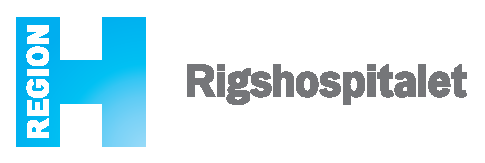
\includegraphics[height=10mm,keepaspectratio]{figures/Logo_Rigshospitalet_CMYK.eps}}; 
    \end{tikzpicture}
    
    % Stanford logo
    \begin{tikzpicture}[remember picture,overlay]
    \node[anchor=north east, 
          xshift=-8.9mm, 
          yshift=-8.3mm] 
         at (current page.north east) 
         {\includegraphics[height=10mm,keepaspectratio]{figures/Stanford_Medicine_V-Print.eps}}; 
    \end{tikzpicture}
    
    % DTU department (to change see Setup/Settings.tex) 
    \begin{tikzpicture}[remember picture,overlay]
    \node[anchor=south west, 
          xshift=8.9mm, 
          yshift=8.3mm] 
          at (current page.south west) 
          {
          \includegraphics[height=10mm,keepaspectratio]{figures/DTU Sundhedsteknologi_UK_highdpi.png}
            % \begingroup
            %     \renewcommand{\arraystretch}{0.8}
            %     \fontfamily{Arial}\selectfont \sffamily
            %     % \color{CTtitle}
            %     \begin{tabular}{l}
            %         \textbf{DTU Health Tech} \\
            %         \myFaculty
            %         % {\fontfamily{Arial}\selectfont \textbf{\textsf{DTU Health Tech}}} \\
            %         % {\fontfamily{Arial}\selectfont \textsf{\myFaculty}}
            %     \end{tabular}
            % \endgroup
            % \color{CTtitle}
            % \begin{tabular}{r} 
            % % \renewcommand{\arraystretch
            % {\fontfamily{Arial}\selectfont \textbf{\textsf{DTU Health Tech}}} \\
            % {\fontfamily{Arial}\selectfont \textsf{\myFaculty}}
            % \end{tabular}
          }; 
    \end{tikzpicture}

\begin{adjustwidth*}{}{-\marginparwidth-\marginparsep}
\begin{center}

    \vfill
    
    \begingroup
        \Huge
        % \fontfamily{helvet}\selectfont
        {\fontfamily{Helvetica}\selectfont \sffamily \textbf{Deep Learning Methods\\for Clinical Sleep Analysis}}
        % \normalfont \myTitle
        % \color{CTtitle}\textbf{\myTitle}
        % \color{CTtitle}\spacedallcaps{\myTitle}
    \endgroup
    
    \bigskip 
    
    \bigskip
    
    \begingroup
        \LARGE
        % \fontfamily{helvet}\selectfont
        % {\fontfamily{Helvetica}\selectfont \sffamily \textbf{\myTitle}}
        % \normalfont \myTitle
        % \color{CTtitle}\textbf{\myTitle}
        % \color{CTtitle}\spacedallcaps{\myTitle}
        {\fontfamily{Helvetica}\selectfont \sffamily \myName}
    \endgroup
    
    % \spacedlowsmallcaps{\myName}
    
    \bigskip
    
    \begingroup
        \Large
        % \fontfamily{helvet}\selectfont
        % {\fontfamily{Helvetica}\selectfont \sffamily \textbf{\myTitle}}
        % \normalfont \myTitle
        % \color{CTtitle}\textbf{\myTitle}
        % \color{CTtitle}\spacedallcaps{\myTitle}
        {\fontfamily{Helvetica}\selectfont \sffamily \myDocument, \myTime}
    \endgroup
    % \spacedlowsmallcaps{\myDocument, \myTime}
    
    \vfill
    
    \vfill
    
\end{center}
\end{adjustwidth*}
\end{titlepage}

% %*******************************************************
% Titlepage
%*******************************************************

\begin{titlepage}
\thispagestyle{empty}

    % % DTU logo
    % \begin{tikzpicture}[remember picture,overlay]
    % \node[anchor=north west, 
    %       xshift=8.9mm, 
    %       yshift=-8.3mm] 
    %      at (current page.north west) 
    %      {\includegraphics[width=14.75mm,keepaspectratio]{figures/Corporate_Red_CMYK.eps}}; 
    % \end{tikzpicture}
    
    % % RH-Glostrup logo
    % \begin{tikzpicture}[remember picture,overlay]
    % \node[anchor=north, 
    %       xshift=0, 
    %       yshift=-8.3mm] 
    %      at (current page.north) 
    %      {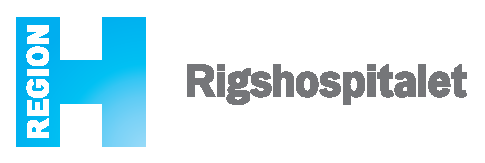
\includegraphics[height=10mm,keepaspectratio]{figures/Logo_Rigshospitalet_CMYK.eps}}; 
    % \end{tikzpicture}
    
    % % Stanford logo
    % \begin{tikzpicture}[remember picture,overlay]
    % \node[anchor=north east, 
    %       xshift=-8.9mm, 
    %       yshift=-8.3mm] 
    %      at (current page.north east) 
    %      {\includegraphics[height=10mm,keepaspectratio]{figures/Stanford_Medicine_V-Print.eps}}; 
    % \end{tikzpicture}
    
    % % DTU department (to change see Setup/Settings.tex) 
    % \begin{tikzpicture}[remember picture,overlay]
    % \node[anchor=south west, 
    %       xshift=5mm, 
    %       yshift=8.3mm] 
    %       at (current page.south west) 
    %       {
    %         \begingroup
    %             \renewcommand{\arraystretch}{0.8}
    %             \fontfamily{Arial}\selectfont \sffamily
    %             % \color{CTtitle}
    %             \begin{tabular}{l}
    %                 \textbf{DTU Health Tech} \\
    %                 \myFaculty
    %                 % {\fontfamily{Arial}\selectfont \textbf{\textsf{DTU Health Tech}}} \\
    %                 % {\fontfamily{Arial}\selectfont \textsf{\myFaculty}}
    %             \end{tabular}
    %         \endgroup
    %         % \color{CTtitle}
    %         % \begin{tabular}{r} 
    %         % % \renewcommand{\arraystretch
    %         % {\fontfamily{Arial}\selectfont \textbf{\textsf{DTU Health Tech}}} \\
    %         % {\fontfamily{Arial}\selectfont \textsf{\myFaculty}}
    %         % \end{tabular}
    %       }; 
    % \end{tikzpicture}

    %\pdfbookmark[1]{\myTitle}{titlepage}
    % if you want the titlepage to be centered, uncomment and fine-tune the line below (KOMA classes environment)
    \begin{adjustwidth*}{}{-\marginparwidth-\marginparsep}
    \begin{center}
        \large

        \hfill

        \vfill

        \begingroup
            \color{CTtitle}\spacedallcaps{\myTitle} \\ \bigskip
        \endgroup

        \spacedlowsmallcaps{\myName}

        \vfill

        \includegraphics[width=6cm]{figures/Grey_CMYK.pdf} \\ \medskip

        \mySubtitle \\ \medskip
        \myDocument, \myTime \\
        \myDepartment \\
        \myFaculty \\
        \myUni \\ \bigskip

        % \myTime
        Supervisors: \\
        Main supervisor, \myProf \\
        Clinical supervisor, \myOtherProf \\
        Clinical supervisor, \mySupervisor \\

        \vfill
        
        % \

    \end{center}
  \end{adjustwidth*}
\end{titlepage}

% \thispagestyle{empty}


\begin{adjustwidth*}{}{-\marginparsep-\marginparwidth}

\hfill

\vfill

\noindent\myName: \textit{\myTitle,} \mySubtitle, %\myDegree, \textcopyright\ 
\myTime

\bigskip

\noindent\spacedlowsmallcaps{Supervisors}: \\
Main supervisor, \myProf \\
Clinical supervisor, \myOtherProf \\
Clinical supervisor, \mySupervisor \\

\medskip

\noindent\spacedlowsmallcaps{Location}: \\
\myLocation

\medskip

\noindent\spacedlowsmallcaps{Time Frame}: \\
December 2016--\myTime

\bigskip
% \noindent This thesis was prepared with \texttt{\classicthesis} for digital use only and is best viewed on a two-page display.
\noindent This thesis was prepared with \texttt{\classicthesis} for print use only.

\end{adjustwidth*}
% \frieze
\cleardoublepage%*******************************************************
% Table of Contents
%*******************************************************
\pagestyle{scrheadings}
\phantomsection
\pdfbookmark[1]{\contentsname}{tableofcontents}
\setcounter{tocdepth}{2} % <-- 2 includes up to subsections in the ToC
\setcounter{secnumdepth}{3} % <-- 3 numbers up to subsubsections
\manualmark
\markboth{\spacedlowsmallcaps{\contentsname}}{\spacedlowsmallcaps{\contentsname}}
\tableofcontents
\automark[section]{chapter}
\renewcommand{\chaptermark}[1]{\markboth{\spacedlowsmallcaps{#1}}{\spacedlowsmallcaps{#1}}}
\renewcommand{\sectionmark}[1]{\markright{\textsc{\thesection}\enspace\spacedlowsmallcaps{#1}}}
%*******************************************************
% List of Figures and of the Tables
%*******************************************************
\clearpage
% \pagestyle{empty} % Uncomment this line if your lists should not have any headlines with section name and page number
\begingroup
    \let\clearpage\relax
    \let\cleardoublepage\relax
    %*******************************************************
    % List of Figures
    %*******************************************************
    \phantomsection
    \addcontentsline{toc}{chapter}{\tocEntry{\listfigurename}}
    \pdfbookmark[1]{\listfigurename}{lof}
    \listoffigures

    \vspace{8ex}

    %*******************************************************
    % List of Tables
    %*******************************************************
    \phantomsection
    \addcontentsline{toc}{chapter}{\tocEntry{\listtablename}}
    \pdfbookmark[1]{\listtablename}{lot}
    \listoftables

    \vspace{8ex}
    \newpage

    %*******************************************************
    % List of Listings
    %*******************************************************
    %\phantomsection
    % \addcontentsline{toc}{chapter}{\lstlistlistingname}
    % \pdfbookmark[1]{\lstlistlistingname}{lol}
    % \lstlistoflistings

    % \vspace{8ex}

    %*******************************************************
    % Acronyms
    %*******************************************************
    \phantomsection
    \addcontentsline{toc}{chapter}{\tocEntry{Acronyms}}
    \pdfbookmark[1]{Acronyms}{acronyms}
    \markboth{\spacedlowsmallcaps{Acronyms}}{\spacedlowsmallcaps{Acronyms}}
    \chapter*{Acronyms}
    \begin{acronym}[SOREMP]
        \acro{AASM}{American Academy of Sleep Medicine}
        \acro{AHI}{apnea/hypopnea index}
        \acro{ASDA}{American Sleep Disorders Association}
        \acro{ANOVA}{analysis of variance}
        \acro{AR}{arousal}
        \acro{bGRU}{bidirectional gated recurrent unit}
        \acro{CNN}{convolutional neural network}
        \acro{CSA}{central sleep apnea}
        \acro{CSF}{cerebrospinal fluid}
        \acro{ECG}{electrocardiography}
        \acro{EEG}{electroencephalography}
        \acro{EMG}{electromyography}
        \acro{EOG}{electrooculography}
        \acro{GP}{Gaussian process}
        \acro{GRU}{gated recurrent unit}
        \acro{HLA}{human leukocyte antigen}
        \acro{ICC}{intraclass correlation coefficient}
        \acro{ICSD-3}{International Classification of Sleep Disorders, \nth{3} edition}
        \acro{IoU}{intersection over union}
        \acro{ISRUC}{Something}
        \acro{LM}{limb movement}
        \acro{MASSCv1}{multi-modal automatic sleep stage classification version 1}
        \acro{MASSCv2}{multi-modal automatic sleep stage classification version 2}
        \acro{MrOS}{MrOS Sleep Study}
        \acro{MSED}{multi-modal sleep event detection}
        \acro{MSL}{mean sleep latency}
        \acro{MSLT}{multiple sleep latency test}
        \acro{N1}{non-rapid eye movement stage 1}
        \acro{N2}{non-rapid eye movement stage 2}
        \acro{N3}{non-rapid eye movement stage 3}
        \acro{NREM}{non-rapid eye movement}
        \acro{NSRR}{National Sleep Research Resource}
        \acro{NT1}{narcolepsy type 1}
        \acro{NT2}{narcolepsy type 2}
        \acro{OSA}{obstructive sleep apnea}
        \acro{PLM}{periodic leg movement}
        \acro{PLMI}{periodic leg movement index}
        \acro{PLMS}{periodic leg movement in sleep}
        \acro{PSG}{polysomnography}
        \acro{RBD}{REM sleep behaviour disorder}
        \acro{RDI}{respiratory disturbance index}
        \acro{REM}{rapid eye movement}
        \acro{ReLU}{rectified linear unit}
        \acro{RFE}{recursive feature elimination}
        \acro{RNN}{recurrent neural network}
        \acro{ROC}{receiver operating characteristic}
        \acro{SEM}{slow eye movement}
        \acro{SHHS}{Sleep Heart Health Study}
        \acro{SOREMP}{sleep onset REM period}
        \acro{SSC}{Stanford Sleep Cohort}
        \acro{SWA}{slow wave activity}
        \acro{WSC}{Wisconsin Sleep Cohort}
        \acro{W}{wakefulness}
        
        \acroplural{RDI}[RDIs]{respiratory disturbance indices}
    \end{acronym}
    
    \newpage
    
    %*******************************************************
    % Publications
    %*******************************************************
    \phantomsection
    \pdfbookmark[1]{Publications}{publications}
    \addcontentsline{toc}{chapter}{\tocEntry{Publications}}
    \markboth{\spacedlowsmallcaps{Publications}}{\spacedlowsmallcaps{Publications}}
    \chapter*{Publications}%\graffito{This is just an early --~and currently ugly~-- test!}
    The following first-author publications have been published, accepted or submitted during my PhD studies and form the basis of this thesis.\footnote{\(\dagger\) indicates shared first authorship.}
    % This might come in handy for PhD theses: some ideas and figures have appeared previously in the following publications:
    
    %\noindent Put your publications from the thesis here. The packages \texttt{multibib} or \texttt{bibtopic} etc. can be used to handle multiple different bibliographies in your document.
    
    \begin{refsection}[ownpubs]
        % \small
        % \nocite{*} % is local to to the enclosing refsection
        
        \paragraph{Conference papers}
        \begin{itemize}
            \item \fullcite{Olesen2018c}
            \item \fullcite{Olesen2019}
            \item \fullcite{Olesen2020DeepDetection}
        \end{itemize}
        
        \paragraph{Journal papers}
        \begin{itemize}
            \item \fullcite{Stephansen2018}
            \item \fullcite{Olesen2020AutomaticSetting}
            \item \fullcite{Olesen2020MSED}
        \end{itemize}
            % \fullcite{Olesen2018, Olesen2019, Olesen2020b}
        % \nocite{Olesen2018c,Stephansen2018,Olesen2019,Olesen2020AutomaticSetting, Olesen2020DeepDetection}
        % \printbibliography[heading=none]
    \end{refsection}
    
    % \begin{refsection}[ownpubs]
    %     \small
    %     % \nocite{*} % is local to to the enclosing refsection
    %     \nocite{Olesen2018c,Stephansen2018,Olesen2019,Olesen2020AutomaticSetting, Olesen2020DeepDetection}
    %     \printbibliography[heading=none]
    % \end{refsection}
    
    
    Furthermore, I have (co-)authored the following publications during my PhD, that although relevant, do not form basis of this thesis.
    
    \begin{refsection}[ownpubs]
        % \small
        % \nocite{*} % is local to to the enclosing refsection
        \paragraph{Journal papers}
            \begin{itemize}
                \item \fullcite{Olesen2018}
                \item \fullcite{Cesari2018}
                \item \fullcite{Carvelli2020}
                \item \fullcite{Brink-Kjaer2019}
            \end{itemize}
            
        \paragraph{Conference papers}
        \begin{itemize}
            \item \fullcite{Klok2018}
        \end{itemize}
        
        \paragraph{Abstracts}
        \begin{itemize}
            \item \fullcite{Brink-Kjaer2018}
            \item \fullcite{Carvelli2018}
            \item \fullcite{Jacobsen2018}
            \item \fullcite{Olesen2018a}
            \item \fullcite{Olesen2019a}
            \item \fullcite{Thybo2020}
        \end{itemize}
        
    \end{refsection}
    
    % \begin{refsection}[ownpubs]
    %     \small
    %     % \nocite{*} % is local to to the enclosing refsection
    %     \paragraph{Conference papers}
    %         \nocite{Klok2018}
    %     \printbibliography[heading=none]
    % \end{refsection}
    
    % \begin{refsection}[ownpubs]
    %     \small
    %     % \nocite{*} % is local to to the enclosing refsection
    %     \paragraph{Abstracts}
    %         \nocite{Brink-Kjaer2018, Carvelli2018, Jacobsen2018, Olesen2020a, Olesen2019a}
    %     \printbibliography[heading=none]
    % \end{refsection}
    
    % \begin{refsection}[ownpubs]
    %     \small
    %     % \nocite{*} % is local to to the enclosing refsection
    %     \paragraph{Journal papers}
    %         \nocite{Olesen2018, Cesari2018, Carvelli2020, Brink-Kjaer2019}
    %         \nocite{Olesen2018, Olesen2018a, Olesen2019a, Jacobsen2018, Carvelli2018, Cesari2018, Carvelli2020, Brink-Kjaer2018, Brink-Kjaer2019, Klok2018}
    %     \printbibliography[heading=none]
    % \end{refsection}
    
    Lastly, I have also written a popular science article about my research titled \textit{Intelligente algoritmer indtager søvnklinikken} for the Danish magazine \textit{Medicoteknik}, which is scheduled for publication in April 2020.

\endgroup

% \cleardoublepage\include{frontbackmatter/Dedication}
%\cleardoublepage\include{frontbackmatter/Foreword}
% \cleardoublepage\include{frontbackmatter/abstract}
% \cleardoublepage%*******************************************************
% Declaration
%*******************************************************
\pdfbookmark[0]{Preface}{preface}
\addcontentsline{toc}{chapter}{\tocEntry{Preface}}
\chapter*{Preface}
\thispagestyle{empty}
Put your preface here.
\bigskip

\noindent\textit{\myLocation, \myTime}

\smallskip

\begin{flushright}
    \begin{tabular}{m{5cm}}
        \\ \hline
        \centering\myName \\
    \end{tabular}
\end{flushright}

% \cleardoublepage%*******************************************************
% Acknowledgments
%*******************************************************
\pdfbookmark[1]{Acknowledgments}{acknowledgments}
\addcontentsline{toc}{chapter}{\tocEntry{Acknowledgements}}

% \begin{flushright}{\slshape
%     We have seen that computer programming is an art, \\
%     because it applies accumulated knowledge to the world, \\
%     because it requires skill and ingenuity, and especially \\
%     because it produces objects of beauty.} \\ \medskip
%     --- \defcitealias{knuth:1974}{Donald E. Knuth}\citetalias{knuth:1974} \citep{knuth:1974}
% \end{flushright}



\bigskip

\begingroup
\let\clearpage\relax
\let\cleardoublepage\relax
\let\cleardoublepage\relax
\chapter*{Acknowledgments}
% \vspace{3cm}
\vfill

First of all, I would like to express my deepest gratitude to my main supervisor \emph{Helge B. D. Sørensen}, and clinical co-supervisors \emph{Poul Jennum}, and \emph{Emmanuel Mignot}, for believing in me and allowing me to work on something that I truly enjoy. 
Thank you for your guidance and support during the last three and a half years.

I would also like to thank all the people associated with the Sleep Lab at Stanford University for welcoming me into their impressive scientific environment, in particular \emph{Eileen Leary}, \emph{Hyatt Moore}, and \emph{Aditya Ambati}; a big thanks to \emph{Stephanie Lettieri} for all your help in general; and also my fellow visiting student researcher \emph{Stanislas Chambon} for engaging and enlightening discussions about machine learning, and for convincing me to switch to PyTorch.

Thank you to all my colleagues at the Section for Health Technology for interesting scientific discussions in our biweekly meetings; my fellow PhD students \emph{Matteo Cesari}, \emph{Mads Olsen}, \emph{Umaer Hanif}, \emph{Andreas Brink-Kjær}, and \emph{Søren Møller Rasmussen} for all of our scientific discussions, and for making sure that I get enough coffee.
A particular thanks goes to \emph{Julie A. E. Christensen}.
Thank you for your friendship and for always being willing to offer scientific insights and inputs to manuscripts and projects.

A huge thanks goes out to all of the students that I have been engaged with during my time at Stanford: \emph{Lorenzo}, \emph{Andreas}, \emph{Kristina}, \emph{Rasmus}, \emph{Jonathan}, \emph{Jakob}, \emph{Thomas}, \emph{Vicente}, \emph{Aske}, and \emph{Joakim}; many of whom have become good friends, and some even my fellow PhD students.
I hope you learned as much from me as I learned from you.
Especially, I would like to express my gratitude towards \emph{Jens. B. Stephansen}, who invited me to work with him on the narcolepsy detector, which has been an incredible experience.

I would also like to extend a huge thanks to \emph{Matteo Cesari}, \emph{Martin Nørgaard}, \emph{Sebastian Holst}, \emph{Rasmus Malik Thaarup Høegh}, and \emph{Julie A. E. Christensen}. 
You have provided valuable comments to this thesis.

To all my friends and family: you have been sorely missed, and I can't wait to hang out and spend time with you all again pending no further restrictions due to corona-virus.
A big thank you to my wonderful in-laws, \emph{Annette \& Amr}, for allowing me to set up a make-shift office in your dining room and babysitting Theodor during the corona-crisis.
To my father \emph{Lars-Ulrik}; thank you for always believing in me, for your guidance and our lunches together at DTU. 
% To my mother \emph{Helle}, who is not with us anymore; I miss you and I hope this will make you proud.

And finally, from the bottom of my heart; I want to acknowledge and thank \emph{Alexandra}, the love of my life, for your enthusiasm and willingness to go on an adventure and live in California for almost two years while carrying our first child; for your infinite patience, resilience, love and understanding while I tried my hands at science---without you, this would not have been possible.

% \begin{itemize}
%     \item Supervisors
%     \item Biomedical signal processing group
%     \item Stanford team
%     \item Fiancee
%     \item In-laws for letting me use their dining room as a temporary office during the coronavirus outbreak.
% \end{itemize}

% Many thanks to everybody who already sent me a postcard!

% Regarding the typography and other help, many thanks go to Marco
% Kuhlmann, Philipp Lehman, Lothar Schlesier, Jim Young, Lorenzo
% Pantieri and Enrico Gregorio\footnote{Members of GuIT (Gruppo
% Italiano Utilizzatori di \TeX\ e \LaTeX )}, J\"org Sommer,
% Joachim K\"ostler, Daniel Gottschlag, Denis Aydin, Paride
% Legovini, Steffen Prochnow, Nicolas Repp, Hinrich Harms,
% Roland Winkler, Jörg Weber, Henri Menke, Claus Lahiri,
% Clemens Niederberger, Stefano Bragaglia, Jörn Hees,
% Scott Lowe, Dave Howcroft, Jos\'e M. Alcaide, David Carlisle,
% Ulrike Fischer, Hugues de Lassus, Csaba Hajdu, Dave Howcroft, 
% and the whole \LaTeX-community for support, ideas and
% some great software.

% \bigskip

% \noindent\emph{Regarding \mLyX}: The \mLyX\ port was intially done by
% \emph{Nicholas Mariette} in March 2009 and continued by
% \emph{Ivo Pletikosi\'c} in 2011. Thank you very much for your
% work and for the contributions to the original style.


\endgroup

% \cleardoublepage%*******************************************************
% Publications
%*******************************************************
\phantomsection
\pdfbookmark[1]{Publications}{publications}
\addcontentsline{toc}{chapter}{\tocEntry{Publications}}
\chapter*{Publications}%\graffito{This is just an early --~and currently ugly~-- test!}
The following publications have been published, accepted or submitted during my PhD and form the basis of this thesis.
% This might come in handy for PhD theses: some ideas and figures have appeared previously in the following publications:

%\noindent Put your publications from the thesis here. The packages \texttt{multibib} or \texttt{bibtopic} etc. can be used to handle multiple different bibliographies in your document.

\begin{refsection}[ownpubs]
    \small
    % \nocite{*} % is local to to the enclosing refsection
    \nocite{Olesen2018c,Stephansen2018,Olesen2019,Olesen2020AutomaticSetting, Olesen2020DeepDetection}
    \printbibliography[heading=none]
\end{refsection}

Furthermore, I have (co-)authored the following publications during my PhD, that do not form basis of this thesis.

\begin{refsection}[ownpubs]
    \small
    % \nocite{*} % is local to to the enclosing refsection
    \nocite{Olesen2018, Olesen2018a, Olesen2019a, Jacobsen2018, Carvelli2018, Cesari2018, Carvelli2020, Brink-Kjaer2018, Brink-Kjaer2019, Klok2018}
    \printbibliography[heading=none]
\end{refsection}

% \emph{Attention}: This requires a separate run of \texttt{bibtex} for your \texttt{refsection}, \eg, \texttt{ClassicThesis1-blx} for this file. You might also use \texttt{biber} as the backend for \texttt{biblatex}. See also \url{http://tex.stackexchange.com/questions/128196/problem-with-refsection}.

%********************************************************************
% Mainmatter
%*******************************************************
\cleardoublepage
\pagestyle{scrheadings}
\pagenumbering{arabic}
%\setcounter{page}{90}
% use \cleardoublepage here to avoid problems with pdfbookmark
\cleardoublepage




\part{Introduction}\label{part:introduction}
% \newcommand{\hypothesis}{Advanced biomedical signal processing and machine learning algorithms can be used for efficient, high-performing analysis of sleep studies.}
% \acresetall
\chapter{Thesis introduction}\label{chap:thesis-introduction}

\begin{flushright}{\slshape 
        Quantum carburetor? Jesus, Morty, you can't just add a sci-fi word to a car word and hope it means something.} \\ \medskip
        --- Rick Sanchez\\Rick and Morty, season 2, episode 6.
\end{flushright}
\vspace{6cm}

Although sleep is essential for normal human brain development and functionality, sleep disorders are prevalent in society.
There are approximately 90 different sleep disorders currently recognized and described in the \ac{ICSD} grouped into six categories: insomnias, circadian rhythm sleep-wake disorders, central hypersomnias (\eg narcolepsy), sleep-related breathing disorders (\eg obstructive sleep apnea), parasomnias (\eg sleepwalking, \acl{RBD}), and sleep-related movement disorders (\eg \acl{PLMD} and restless legs syndrome)~\cite{AmericanAcademyofSleepMedicine2014}.
It is estimated that about 25\% of the US population present with sleep apnea-related symptoms~\cite{Young2002, Gottlieb2020} with similar prevalences in other developed countries~\cite{Tufik2010, Heinzer2015, Arnardottir2016, Fietze2019}.
The prevalence of chronic insomnia is estimated to be about 10\% of the US population~\cite{Ozminkowski2007}, and 6\% in high-income countries~\cite{Ohayon2002}---a number increasing to up to 48\% when including insomnia symptoms alone~\cite{Ohayon2002}. 
Although these numbers are high, evidence suggests that sleep disorders are severely under-diagnosed~\cite{Decker2008, Ohayon2011, Johnson2018}. 

Disrupted sleep is associated with increased risk of developing systemic hypertension, cardiovascular disease and abnormalities in the metabolism~\cite{Punjabi2008}.
Increased levels of fatigue due to disrupted nighttime sleep is also a cause of motor-vehicle accidents~\cite{Lyznicki1998}, as people with excessive daytime sleepiness have a sevenfold greater risk of being involved in an accident~\cite{Findley1988}.

Apart from the medical impacts on a personal level, sleep disorders have monumental societal impact due to their prevalence and cost of care.
A study on the burden of poor sleep in the Australian population estimated the annual economic cost at \$42.5 billion~\cite{Hillman2006}, while the combined cost of poor sleep in USA, Canada, UK, Japan and Germany is estimated to exceed \$600 billion per year~\cite{Hafner2017}. 
USA alone accounts for an estimated \$411 billion of these costs~\cite{Kiley2019}.

Currently, the gold standard of diagnosing sleep disorders is based on manual analysis of sleep patterns following the guidelines published by the \ac{AASM} and the clinical guidelines in the~\ac{ICSD}~\cite{AmericanAcademyofSleepMedicine2014}.
Sleep is recorded in sleep clinics using \ac{PSG}, which comprises several recording modalities across the body\graffito{Specific details concerning \ac{PSG} setup and recording will be described in~\cref{sec:recording-quantifying-sleep}.}.
% covers multiple modalities such as \ac{EEG} for recording brain activity, \ac{EOG} for eye movements, \ac{EMG} for chin and limb muscle activity, \ac{ECG} for heart activity, respiratory inductance plethysmopgrahy belts on the thorax and abdomen, and pulse oximetry for measuring blood oxygen content.
Patients in the sleep clinic wear and sleep with a heavy and extensive recording setup, which may have an impact on regular sleep patterns~\cite{Agnew1966, Scholle2003}.

Apart from being time consuming and cumbersome for both patients and clinical personnel, there is growing evidence\graffito{These findings on variability will be presented in~\cref{sec:challenges-scoring-sleep-studies}.} that manual analysis of sleep patterns suffer from subjectiveness resulting in high inter-scorer variabilities~\cite{Drinnan1998, Whitney1998, Danker-Hopfe2004, Norman2000, Magalang2013, Rosenberg2013, Rosenberg2014, Younes2016, Younes2018}.
In the last decades, there has been an increasing effort to come up with new solutions that can ease and standardize the way sleep data is acquired and analyzed. 
% Due to these issues, there is an increasing effort to come up with solutions that can tackle these problem areas both in terms of data acquisition and data analysis.

\begin{figure}
\begin{adjustwidth*}{}{-\marginparwidth-\marginparsep}
    \centering
    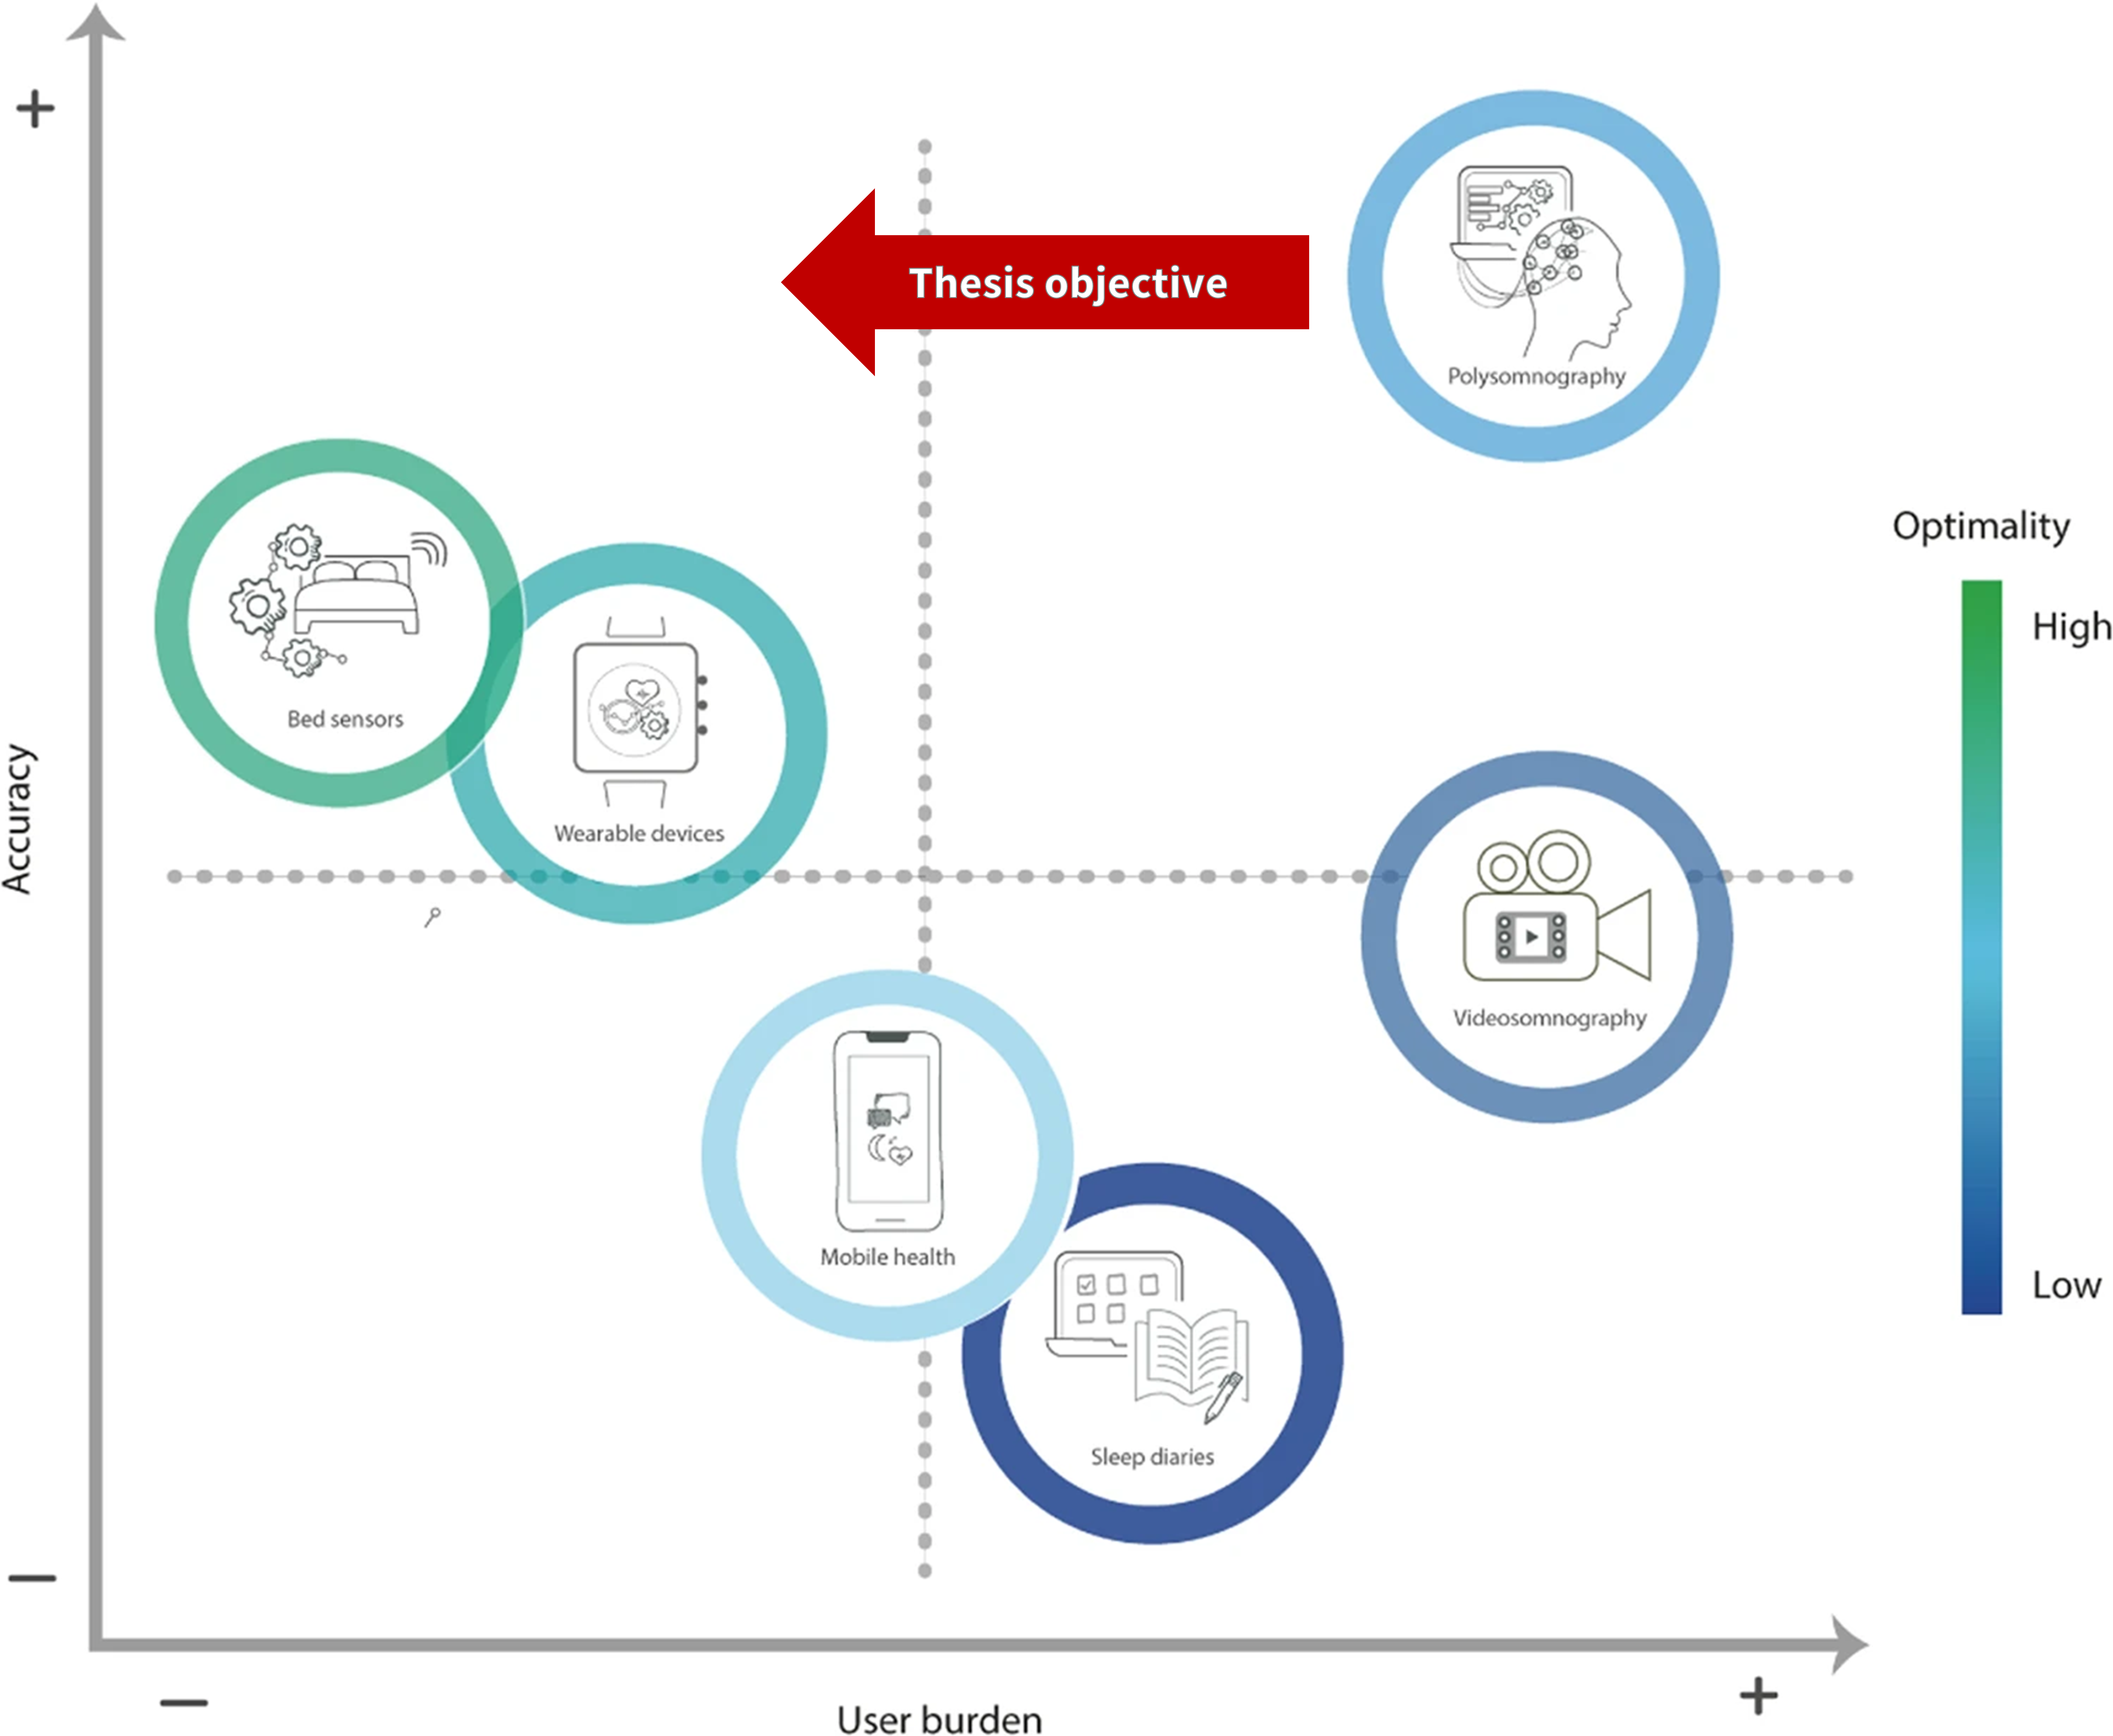
\includegraphics[width=0.95\linewidth]{figures/introduction/npjFig3_objective.png}
    \caption[Accuracy-usability trade-off in sleep analysis]{Accuracy-usability trade-off for selected methods in sleep analysis. Polysomnography is considered the gold standard in sleep medicine providing high levels of accuracy, while also being very cumbersome and time-consuming. Videosomnography provides lower levels of accuracy, while being equally cumbersome and time-consuming, although this is required for diagnosis of some sleep disorders. User-centered technologies such as health apps and sleep diaries are easier to use than the gold standard methods, but are generally not accurate in capturing sleep metrics. Wearable devices and ubiquitous technologies, such as bed and radiowave sensors, generally have the lowest impact on the user, while providing medium levels of accuracy. This thesis will focus on improving the the gold standard indicated on the figure by moving polysomnography along the red arrow to the left along the user burden axis. In this case, user burden encompasses both the burden to the patient, as well as the burden to the clinician. Adapted from~\cite{Perez-Pozuelo2020} under a Creative Commons Attributes 4.0 International License: \url{http://creativecommons.org/licenses/by/4.0/}.}
    \label{fig:introduction:figure-02}
\end{adjustwidth*}
\end{figure}

% On the acquisition side, n
Numerous commercial, industrial and academic interests are focusing on easier methods for acquiring sleep data in the form of mobile health applications and low-cost wearable/nearable devices\graffito{\emph{Nearables} include non-contact devices such as radar-based sensing, and embedded sensors such as bed sensors.} such as headbands, in-ear \ac{EEG}, or activity trackers~\cite{Perez-Pozuelo2020}.
These devices are interesting from several standpoints, but mostly due to the low user burden compared to conventional \ac{PSG}.
However, wearable devices are not yet applied in clinical practice, due to the limited validation against gold standard methods~\cite{Depner2019}.
This trade-off between usability and user burden versus accuracy is depicted graphically in~\cref{fig:introduction:figure-02} for several methods available for sleep recording and/or quantification.% of sleep.

Similarly, numerous efforts have already been made on the data analysis side to automate the sleep analysis process.
Especially the task of automatic sleep stage classification has been the subject of many research papers~\cite{Sen2014}.
With the rising presence of artificial intelligence in medicine, and deep learning in particular~\cite{LeCun2015, Yu2018, He2019}, more and more research groups are focusing on applying advanced signal processing and analysis techniques to sleep data.
Due to the vast number of different approaches regarding the number of classified sleep stages, feature extraction, classification algorithms, applied datasets, and validation approaches, direct comparison between published findings is a complex task~\cite{Ronzhina2012, Sen2014, Radha2014, Aboalayon2016, Boostani2017}.
However, high quality large-scale studies on automatic methods for sleep analysis was until very recently not dominant in the literature.
% \paragraph{Missing paragraphs}
% \begin{itemize}
%     \item Introduction to sleep science?
%     \item Introduce some papers on automating clinical sleep scoring, state of the art
%     \item (Need for objective measures since perceptions of sleep are highly subjective: 1. Hermans LWA, van Gilst MM, Regis M, et al. Modeling sleep onset misperception in insomnia. Sleep. 2020:1-10. doi:10.1093/sleep/zsaa014 \cite{Hermans2020})
%     \item New technologies for sleep analysis \cite{Perez-Pozuelo2020}
% \end{itemize}



% \begin{figure}
%     % \begin{adjustwidth*}{}{-\marginparwidth-\marginparsep}
%     \myfloatalign   
%     \subfloat[]
%     {\includegraphics[width=0.49\textwidth + 0.49\marginparwidth + 0.49\marginparsep]{figures/introduction/41746_2020_244_Fig2_HTML.pdf}} \\
%     \subfloat[]
%     {\includegraphics[width=0.49\textwidth + 0.49\marginparwidth + 0.49\marginparsep]{figures/introduction/41746_2020_244_Fig3_HTML.pdf}}
%     \caption{}
%     \label{fig:introduction:figure-01}
%     % \end{adjustwidth*}
% \end{figure}


\section{Problem statement and research hypothesis}
Analysis of sleep is based on manual scoring of \acp{PSG} recorded overnight at either a sleep clinic or at home, which are prone to subjective interpretation of scoring rules.
Correct identification and analysis of sleep patterns precedes correct diagnosis and thus subsequent treatment of sleep disorders.
\textbf{The objective of this thesis is}
\begin{quote}
    % \emph{to develop a system based on artificial intelligence, that can assist clinicians in the analysis of sleep studies.}
    \emph{\objective.}
    % \emph{to develop a system based on artificial intelligence to assist medical and technical experts in automatic analysis of sleep studies.}
\end{quote}
The aim is to ease the way \acp{PSG} are analyzed in the clinic today, but without lowering accuracy.
This is depicted graphically in~\cref{fig:introduction:figure-02} by moving the \ac{PSG} along the red arrow.
% \emph{to develop a system based on artificial intelligence to assist medical and technical experts in automatic analysis of sleep studies}.
% This is depicted graphically in~\cref{fig:introduction:figure-02} by moving the user burden of \ac{PSG} along the red arrow while maintaining high levels of accuracy.

% Taking into account the motivation, the problem statement is formalized into three separate research hypotheses:
Taking into account the motivation, the problem statement is formalized into the following \textbf{thesis hypothesis}:
\begin{quote}
    \hypothesis
\end{quote}
\begin{enumerate}[label={\footnotesize\bfseries\scshape RH~\arabic*}, ref={\bfseries\scshape RH~\arabic*}]
    \item sleep stages;\label{hypothesis:sleep-stages}%\hypothesisSleepStages;\label{hypothesis:sleep-stages}
    \item sleep events;\label{hypothesis:sleep-events} and,%\hypothesisSleepEvents;\label{hypothesis:sleep-events}
    \item sleep disorders.\label{hypothesis:sleep-disorders}%\hypothesisSleepDisorders;\label{hypothesis:sleep-events}
\end{enumerate}


% \section{Research questions and hypotheses}
% Taking into the account the motivation, the problem statement is formalized by the following \emph{thesis hypothesis}:
% \begin{quote}
%     \emph{\hypothesis}
% \end{quote}
% Based on the thesis hypothesis, the following \emph{thesis objectives} are defined:
% \begin{itemize}
%     \item to design a fully automatic sleep stage classification algorithm based on advanced machine learning techniques and validate the utility of such an algorithm in multiple databases.
%     \item to design a flexible sleep event detection algorithm that can both classify and localize sleep events in the \ac{PSG}. The algorithm should be flexible by design to allow for multiple event classes and/or signal inputs.
%     \item to design an algorithm capable of detecting sleep disorders based on a single night of \ac{PSG} recording and validate the utility of such and algorithm in multiple databases.
% \end{itemize}
% \hypothesis
% \begin{enumerate}[label={\footnotesize\bfseries\scshape RH~\arabic*}, ref={\bfseries\scshape RH~\arabic*}]
%     \item sleep stages;\label{hypothesis:sleep-stages}%\hypothesisSleepStages;\label{hypothesis:sleep-stages}
%     \item sleep micro-events; and,\label{hypothesis:sleep-events}%\hypothesisSleepEvents;\label{hypothesis:sleep-events}
%     \item sleep disorders.\label{hypothesis:sleep-disorders}%\hypothesisSleepDisorders;\label{hypothesis:sleep-disorders}.
% \end{enumerate}
% Also write something along the lines that brain activity can be represented by a mixture of states (fuzzy logic, hypnodensity)

\section{Thesis outline and scientific contributions}
\newcommand{\printpublication}[1]{\AtNextCite{\defcounter{maxnames}{99}}\fullcite{#1}}
The scientific content of this research is grouped into three research themes each with its own chapter.
% \begin{enumerate}[label={\footnotesize\bfseries\scshape Chapter~\arabic*}, ref={\bfseries\scshape Chapter~\arabic*}]
%     \item contains the preliminary introduction and motivation to this thesis, and outlines the content (about which you are now reading) and scientific contributions herein.
%     \item provides necessary clinical background for readers with little previous knowledge in somnology and sleep medicine\graffito{\emph{Somnology} is a branch of science devoted to the study of the physiology and behavioral dimensions of sleep, and the personal and population-level effects of poor sleep. \emph{Sleep medicine} is a branch of clinical medicine devoted to the diagnosis and treatment of individuals suffering from chronic sleep loss or sleep disorders.}. 
%     However, this is by now means an exhaustive treatment of the two fields.
%     \item presents three studies on \emph{automatic sleep stage classification} models, the first research theme.
%     \item presents three studies on a model developed for \emph{sleep micro-event detection}, which is the second research theme.
%     \item presents the development of a narcolepsy classification algorithm, based on outputs from one of the sleep stage classification models presented in \textbf{Chapter 3}.
%     \item integrates the findings from the three research chapters in a discussion relative to the stated research hypotheses and objectives.
%     \item concludes the thesis by summing up the main research findings.
%     \item outlines some of the future directions and research perspectives in the field of \emph{computational sleep science} related to the themes presented in this thesis.
% \end{enumerate}

\textbf{\cref{chap:thesis-introduction}} contains the preliminary introduction and motivation to this thesis, and outlines the content and scientific contributions.

\textbf{\cref{chap:clinical-background}} provides necessary clinical background for readers with little previous knowledge in somnology and sleep medicine.
%\graffito{\emph{Somnology} is a branch of science devoted to the study of the physiology and behavioral dimensions of sleep, and the personal and population-level effects of poor sleep. \emph{Sleep medicine} is a branch of clinical medicine devoted to the diagnosis and treatment of individuals suffering from chronic sleep loss or sleep disorders.}. 
% However, this is not intended to provide an exhaustive treatment of the two fields.
    
\textbf{\cref{chap:sleep-stage-classification}} presents three studies on \emph{automatic sleep stage classification}, the first research theme.

\textbf{\cref{chap:sleep-event-detection}} presents three studies on a model developed for \emph{sleep micro-event detection}, which is the second research theme.

\textbf{\cref{chap:classification-sleep-disorders}} presents the development of a narcolepsy classification algorithm, based on outputs from one of the sleep stage classification models presented in~\cref{chap:sleep-stage-classification}. This concerns the third and final research theme.

\textbf{\cref{chap:discussion}} integrates the findings of this dissertation in a discussion relative to the stated research hypotheses and objectives.

\textbf{\cref{chap:conclusion}} concludes the thesis by summing up the main research findings.

\textbf{\cref{chap:future-work}} outlines some of the future directions and research perspectives in the field of \emph{computational sleep science}.

\bigskip

The following first-author publications have been published, accepted or submitted during my PhD studies and form the scientific basis of this thesis.\footnote{\(^{\ast}\) indicates shared first authorship.} Preprints and/or published versions of these are supplied in the appendix.
    
\begin{refsection}[ownpubs]
    \small
    
    \paragraph{Journal papers}
    \begin{itemize}[label=--]
        \item \printpublication{Stephansen2018}
        \item \printpublication{Olesen2020AutomaticSetting}
        \item \printpublication{Olesen2020MSED}
    \end{itemize}
    
    \paragraph{Conference papers}
    \begin{itemize}[label=--]
        \item \printpublication{Olesen2018c}
        \item \printpublication{Olesen2019}
        \item \printpublication{Olesen2020DeepDetection}
    \end{itemize}
\end{refsection}

\noindent Furthermore, I have (co-)authored the following publications during my PhD.%, that although relevant, do not form basis of this thesis.

\begin{refsection}[ownpubs]
    \small
    \paragraph{Journal papers}
        \begin{itemize}[label=--]
            \item \printpublication{Olesen2018}
            \item \printpublication{Cesari2018}
            \item \printpublication{Brink-Kjaer2020}
            \item \printpublication{Carvelli2020}
            \item \printpublication{Ambati2020}
        \end{itemize}
        
    \paragraph{Conference papers}
    \begin{itemize}[label=--]
        \item \printpublication{Klok2018}
    \end{itemize}
    
    \paragraph{Abstracts}
    \begin{itemize}[label=--]
        \item \printpublication{Brink-Kjaer2018}
        \item \printpublication{Carvelli2018}
        \item \printpublication{Jacobsen2018}
        \item \printpublication{Olesen2018a}
        \item \printpublication{Olesen2019a}
        \item \printpublication{Thybo2020}
    \end{itemize}
    
\end{refsection}


\noindent Finally, I have also written a popular science article about my research titled \emph{Intelligente algoritmer på søvnklinikken} (Intelligent algorithms in the sleep clinic) for the Danish industry magazine \emph{Medicoteknik}.\cleardoublepage
\acresetall
\chapter{Clinical background}\label{chap:clinical-background}
\begin{flushright}{\slshape 
        What, so everyone’s supposed to sleep every single night now? You realize that nighttime makes up half of all time?} \\ \medskip
        --- Rick Sanchez\\Rick and Morty, season 1, pilot episode
\end{flushright}
\vspace{6cm}
    
    This chapter aims to provide the reader with a basic and preliminary understanding of sleep science. 
    First, the fundamental aspects of sleep as a physiological phenomenon is reviewed. Unless otherwise stated, the context will be concerning sleep in primarily healthy adults. 
    This will be followed by a description of how sleep is recorded, quantified and analyzed in clinical practice.
    Then, a brief overview of common sleep disorders relevant to the topic of this thesis will be provided.
    The chapter will conclude with a section on some of the major challenges and difficulties that arise in clinical sleep practice, such as inter- and intra-rater variability, and how this can affect clinical outcomes.
    
    \section{Fundamental aspects of sleep}\label{sec:fundamental-aspects-sleep}
    
        Sleeping is ubiqituous to human life, but although we spend almost a third of our time sleeping, there is still many aspects that are unknown to science. 
        However, we have a general understanding of how our sleep is structured, which will be described in the following sections. 
        Sleep is a complex, physiological state, that impacts several aspects of the human physiology, and although our bodies might seem static, it is actually comprised of multiple, very dynamic processes observable across multiple recording modalities.
        
        Described in the following sections are two important concepts of sleep.
        \begin{description}
            \item[Sleep architecture] refers to the structure of sleep, how it is divided into different states based on physiological characteristics, and the dynamics of those states across the night.
            This can also be called \textit{macro-sleep}, as it concerns the overall macro-structure of our sleep patterns.
            \item[Sleep events] are discrete observations with various characteristics that are distinct for the specific event type.
            Many such events can happen during sleep, and the duration and scope of these events can vary from short and localized (leg movements, sleep spindles), to long and broad (arousals, apneas).
            The description and characterization of these events can also be called \textit{micro-sleep}, but this term is also sometimes applied to sleep architecture on a small time-scale.
            In this thesis, I will refer to this concept as either \textit{micro-sleep events} or just \textit{sleep events} for short.
        \end{description}
        
        \subsection{Sleep architecture}\label{sec:sleep-architecture}
            On average, normal sleep in adult humans lasts between 7-9 hours per night with significant variability between persons. 
            During this period, the brain and body cycles between alternating \textit{sleep stages}, which can be categorized into a state of drowsiness or semi-conscious \ac{W} stage, a \ac{REM} sleep stage, and three \ac{NREM} stages, \ac{N1}, \ac{N2}, and \ac{N3}.
            The main distinction between sleep stages comes from the amplitude and spectral content of the brain signals. 
            For example, wakefulness being associated with high frequency, low amplitude content, and the sleeping stages being associated with more low frequency, high amplitude content. 
            An overview of relevant frequency bands and their appearance in the brain signals is shown in~\cref{tab:eeg_rythms} as defined in the review paper by~\cite{Brown2012} as well as definitions from the~\ac{AASM} for clinical practice.
            \begin{table}[tb]
                \centering
            \begin{threeparttable}
                \caption[Clinical EEG frequency bands]{Clinical EEG frequency bands.}
                \label{tab:eeg_rythms}
                \begin{tabular}{@{}lcc@{}} \toprule
                % \begin{tabular}{lc}\toprule
                    \textbf{Rhythm} & \textbf{\citet{Brown2012}} & \textbf{\citet{Berry2020} (\acs{AASM}2020)} \\ \midrule
                    Delta, $\delta$ & \SIrange{1}{4}{\hertz} & \SIrange{0}{3.99}{\hertz} \\
                    \Ac{SWA} & \SIrange{0.5}{4}{\hertz} & \SIrange{0.5}{2.0}{\hertz} \\
                    Theta, $\theta$ & \SIrange{4}{8}{\hertz} & \SIrange{4}{7.99}{\hertz} \\
                    Alpha, $\alpha$ & \SIrange{8}{14}{\hertz} & \SIrange{8}{13}{\hertz} \\
                    Beta, $\beta$ & \SIrange{15}{30}{\hertz} & $>\SI{13}{\hertz}$\\
                    Gamma, $\gamma$ & \SIrange{30}{120}{\hertz} & n.d.\\ \bottomrule
                \end{tabular}
                \begin{tablenotes}
                    \item n.d., not defined.
                \end{tablenotes}
            \end{threeparttable}
            \end{table}
            
            However, certain brain stages are also characterized by the presence of certain micro-structure events with very distinct morphologies, such as sleep spindles or K-complexes in the brain signal recordings, or \acp{REM} in the recordings of eye activity~\citep{Brown2012, Saper2010, Carskadon2011a, Peyron1998}.
            
            The following lists the major electrophysiological findings for the five sleep stages currently defined by the~\ac{AASM}.
            
            % \begin{itemize}
            %     \item[\ac{W}] 
            %     \item[\ac{REM}]
            %     \item[\ac{N1}]
            %     \item[\ac{N2}]
            %     \item[\ac{N3}]
            % \end{itemize}
            
            \subsubsection{Wakefulness}\label{sec:wakefulness}
            Spanning from a full awareness state to a quiet awakening or drowsiness state, this stage generally accounts for about \SI{5}{\percent} of the total time in bed from lights out to lights on in healthy adults.
            In this stage, the brain typically exhibits low amplitude, high frequency content in small areas and more widespread theta rhythms.
            During quiet awakening, these theta rhythms increase in the frontal area, while alpha rhythms are dominant over the occipital region, especially when the eyes are closed.
            With eyes open, this stage is characterized by eye blinking, reading eye movements\graffito{reading eye movements are WHAT} and \acp{REM}.
            The muscle tone is typically high with unspecific amplitude (\textcolor{red}{how much?}).
            
            \subsubsection{NREM sleep}
            Sleep in humans generally commences when a person progresses from \ac{W} to one of the three stages of \ac{NREM}\graffito{Sleep was up until 2007 scored using four stages of \ac{NREM} sleep as defined by Rechtschaffen and Kales.}.
            In general terms, the ordering of \ac{N1}, \ac{N2}, and \ac{N3} respresents a continuum of the depth of sleep, which is primarily constituted by a progressive slowing of the \ac{EEG} activity from predominantly high frequency alpha and theta rhythms with low voltage, to low frequency delta rhythms with large amplitude.
            Furthermore, another major indicator of deepening sleep is the increasing arousal thresholds associated with the progression from \ac{N1} to \ac{N3}.
            
            \paragraph{N1} sleep is usually the first stage to be encountered during sleep, and this stage is generally considered to be a transitional stage between drowsiness and deeper sleep.
            It is characterized by mixed frequency content, as the alpha rhythms are progressively reduced and replaced with theta rhythms.
            Additionally, small sleep events called \textit{vertex sharp waves} also appear in the \ac{EEG} during this stage\graffito{Vertex sharp waves are sharply contoured waveforms with a very short duration of less than \SI{0.5}{\second}}.
            \Acp{REM} and reading eye movements are replaced with slow eye movements and the muscle tone is reduced compared to \ac{W}.
            
            
            Broadly speaking, their ordering represents a depth-of-sleep continuum indicated by both a progression from low voltage, high frequency alpha/theta rythms to large amplitude, low frequency delta rythms (slowing of cortical activity), and by increasing arousal thresholds (Brown et al., 2012; Carskadon and Dement, 2011). They generally constitute approximately 2 % to 5 %, 45 % to 55 %, and 13 % to 23 % of the TST for the first, second, and third NREM stage, respectively.
            
            \subsubsection{REM sleep}
            
                \cite{Foulkes1962, Ermis2010, Sato1997, Hobson2009}
                
            \subsubsection{Neurobiological control of sleep}\label{sec:control-sleep}
        \subsection{Micro-events durings sleep}
            \subsubsection{Arousals}
                \citep{Ermis2010}
            \subsubsection{Movements of the extremities}
            \subsubsection{Respiratory disturbances}
            \subsubsection{K-complexes and sleep spindles}
                \citep{Cash2009, Gennaro2003, Forget2011}
    \section{Recording and quantifying sleep}\label{sec:recording-quantifying-sleep}
        \cite{Berry2020}
        \subsection{Polysomnography}\label{sec:polysomnography}
            The principal tool available to sleep physicians and technicians for analysis of sleep patterns is the \textit{polysomnography} (PSG).
            This is often the first study performed on patients referred to a sleep clinic, and consists of the continuous and concurrent recording of several physiological variables as electrophysiological signals.
            The primary signals of interest are brain activity (electroencephalography, EEG), eye movements (electrooculography, EOG), chin and leg muscle activity (electromyography, EMG), heart activity (electrocardiography, ECG), respiratory effort (thoracoabdominal inductance plethysmography belts, RIP), nasal pressure, oral airflow, and blood oxygen saturation (pulse oximetry).
            Sleep experts manually analyze the contents of these signals in order to score sleep stages and annotate sleep events based on a standardized set of guidelines published by the \ac{AASM}~\cite{AASM2014}. 
            These guidelines also contain technical recommendations for recording sleep studies, such as electrode placements, minimal sampling frequencies and specific filter settings. \cref{tab:aasm_recordings} lists an overview of recommend technical specifications for commonly recorded signals.
            
            A common procedure for analysis of sleep studies involve multiple passes through each PSG study.
            For example, a first pass could be to score every consecutive segment of \SI{30}{\second} data as one of the five sleep stages.
            A second pass could be to score respiratory events, arousals and leg movements, etc. 
            The product of these passes is a sleep study report, which summarizes the findings into a hypnogram and assocated PSG variables, such as total sleep time (TST), sleep latency (SL), REM latency (RL), wake after sleep onset (WASO), percentage of time spent in the different sleep stages.
            Key indices describing the amount of sleep events are also calculated for each study, such as the arousal index (number of arousals per hour of sleep, ArI), apnea-hypopnea index (number of apneas and hypopneas per hour of sleep, AHI), and the periodic limb movements in sleep index (number of peridoc limb movement series in sleep per hour of sleep, PLMSI). 

            \begin{table}[tb]
            \begin{threeparttable}
                \small
                \centering
                \caption[Technical specifications for recording \ac{PSG} signals]{Technical specifications for recording commong signals in \acp{PSG} according to \ac{AASM} standards~\cite{Berry2020}.}% used for subsequent visualization and analysis}
                \label{tab:aasm_recordings}
                \begin{tabular}{@{}llll@{}} \toprule
                    \textbf{Signal} & \textbf{Recommended recording setup} & \textbf{Min.} \(\mathbf{f_s}\) & \textbf{Filter} \\ \midrule
                    EEG & F4-M1, C4-M1, O2-M1 (required)    & \SI{200}{\hertz}  & \SIrange[range-units=single,range-phrase=--]{0.3}{35}{\hertz} \\
                        & F3-M2, C3-M2, O1-M2 (backup)      &                   &                                                               \\
                    EOG & E1-M2, E2-M2 (required)   & \SI{200}{\hertz}  & \SIrange[range-units=single,range-phrase=--]{0.3}{35}{\hertz} \\
                        & E1-M1, E2-M1 (backup)     &                   &                                                               \\
                    EMG & Chin2-ChinZ (required, chin EMG)  & \SI{200}{\hertz}  & \SIrange[range-units=single,range-phrase=--]{10}{100}{\hertz} \\
                        & Chin1-ChinZ (backup, chin EMG)    &                   &                                                               \\
                        & Bipolar derivation (required, leg EMG) & &                                            \\
                    ECG & modified Lead II derivation (required) & \SI{200}{\hertz} & \SIrange[range-units=single,range-phrase=--]{0.3}{70}{\hertz} \\ \bottomrule
                    % RIP & --- & \SI{25}{\hertz} & \SIrange[range-units=single,range-phrase=--]{0.1}{15}{\hertz} \\ 
                    % Nasal pressure & --- & \SI{25}{\hertz} & \SIrange[range-units=single,range-phrase=--]{\leq 0.03}{100}{\hertz} \\ 
                    % Airflow & --- & \SI{25}{\hertz} & \SIrange[range-units=single,range-phrase=--]{0.1}{15}{\hertz} \\ 
                    % Oximetry & --- & \SI{10}{\hertz} & \SIrange[range-units=single,range-phrase=--]{}{15}{\hertz} \\ \bottomrule
                \end{tabular}
            \begin{tablenotes}
            \item  AASM describes a specific requirement as well as a backup in case of failure for each signal. Minimal \( f_s \) lists the minimally acceptable sampling frequency per signal, but the recommendations are higher in order to better capture waveform morphology. Filter settings describe recommended bandpass filter settings
            \end{tablenotes}
            \end{threeparttable}
            \end{table}
            
        % \subsection{Multiple sleep latency test}
        % \subsection{Technical considerations when recording sleep studies}
    % \section{Abnormal sleep and sleep disorders}
        
    %     In the following sections are briefly described some of the common sleep disorders that are relevant to the topic of this thesis.
    %     % A diagnosis of sleep disorders is based on multiple parameters.
    %     Commonly, a patient is submitted to a sleep clinic under suspicion of a sleep disorder under referral from a general practitioner or physician, when they experience extreme tiredness during daylight hours, or perhaps a significant other experience nightly disturbances.
    %     Healthcare professionals make a diagnosis from the medical history, answers to questionnaires, findings from the PSG and/or MSLT, and lab test results, according to diagnostic criteria published by the AASM in~\citetitle{AASM2014}~\cite{AASM2014}.
        
    %     \subsection{Sleep related breathing disorders}
    %     Sleep disordered breathing comprise several disorders and syndromes, but is generally characterized by respiratory problems during sleep and sometimes during wakefulness.
        
    %     \textbf{Obstructive sleep apnea} (OSA) is characterized by recurrent restrictions in the upper airways~\cite{Malhotra2002}.
    %     It is a very common disease with \SIrange[range-units=single,range-phrase=--]{5}{15}{\percent} of the general population in the USA affected by OSA~\cite{Young}. 
        
    %     \subsection{Movement disorders}
        
    %     \subsection{Narcolepsy}
    
    %     \citep{AASM2014}
    \section{Challenges in scoring sleep studies}\label{sec:challenges-scoring-sleep-studies}
        Significant human bias can enter into the analysis of sleep studies by virtue of the process being performed manually.
        Several studies have shown significant \textit{inter-} and \textit{intra-}rater variability\graffito{Interrater variability refers to the variation in scoring that happens between experts on the same study, while intrarater variability refers to the variability in scoring when a single expert scores the same study more than once.} primarily in the case for sleep stage scoring, but some studies have also investigated the reliability of scoring arousals and respiratory events for sleep-related breathing disorders.
        This variability can be caused by several factors:
        \begin{enumerate}
            \item \textit{Imprecise scoring guidelines.}
            Some have argued that extensive training is required to minimize the subjective component in sleep stage scoring, and that the optimal training requires participation in concensus scoring rounds~\cite{Penzel2013}.
            \item \textit{Presence of disease or other sleep disorders.}
            Many neurodegenerative diseases exhibit symptoms of disturbed sleep as the neurodegeneration progresses to the centers in the brain stem responsible for control of sleep and wakefulness.
            Similarly, central hypersomnias can also exhibit fragmented sleep.
            Narcolepsy, for instance, show increased fragmentation of sleep, because the hypocretin-producing cells in the latero-posterior hypothalamus are missing~\cite{Kornum2017a}.
            Since current scoring guidelines are based on clinical experience in healthy subjects exhibiting normal sleep patterns, the scoring of sleep patterns becomes difficult in this context.
            \item \textit{True errors.}
            These can occur when annotations are correctly made, but entered wrongly into a computer system or report. 
            However, these types of errors are difficult to measure in practice.
        \end{enumerate}
        
        Depending on the target variable under investigation, reliability and variability can be measured with different metrics.
        The following sections will describe some of the studies that have investigated inter- and intra-scorer reliability for various sleep analysis objectives.
        
        
        \subsection{Sleep stage scoring}\label{sec:challenges-sleep-stage-scoring}
        
            \citeauthor{Norman2000} found the average epoch by epoch agreement between five experienced PSG technicians representing different clinics to be \SI{73}{\percent} in a dataset containing 62 PSGs~\cite{Norman2000}.
            Furthermore, they also found this agreement to vary with phenotype, as the average agreement in a normal subset was higher than for a subset consisting of patients with sleep disordered breathing (\SI{76}{\percent} in the normal subset vs. \SI{71}{\percent} in the SDB subset).
            
            Later studies also found significant variability in expert agreements when comparing different patient groups. 
            Notably, \citeauthor{Danker-Hopfe2004} investigated interrater reliability between experienced technicians in eight different sleep clinics in Europe in a sample of 196 recordings from 98 patients exhibiting different disorders, such as depression, general anxiety disorder with and without insomnia, Parkinson's disease, sleep apnea and periodic leg movements in sleep disorder~\cite{Danker-Hopfe2004}.
            They found that although the overall agreement between experts as measured by \cohen{}\graffito{\cohen{} is a measure of the observed agreement between two agents taking into account chance agreement.} was \num{0.6816}, there was a statistically significant difference between patient groups, where the median $\kappa$ ranged from \num{0.6138} in patients with Parkinson's disease to \num{0.8176} in patients with generalized anxiety disorder.
            Other studies have found no statistically significant differences in the overall agreement between healthy controls, patients with sleep apnea/hypopnea syndrome, and patients with narcolepsy, when comparing scorers from Berlin and Beijing~\cite{Zhang2015a}. 
            They did, however, find statistically significant differences in the stage-specific agreements between patient groups.
            
            Recent large scale studies on interscorer agreement found that the average consensus-agreement is approximately \SI{83}{\percent} with the overall stage-specific agreement ranging from \SI{63}{\percent} for N1 to \SI{91}{\percent} for REM~\cite{Rosenberg2013}.
            The authors recognize that their results are heavily biased towards agreements in the N2 stage, as this accounts for almost \SI{60}{\percent} of the total number of epochs, however, this percentage is in agreement with clinical experience and reflects the amount of N2 in a typical sleep study.
            
            Although human subjective bias is also a factor, the vast majority of interscorer differences most likely originate from equivocal epochs than have equal probability of being assigned to two stages. 
            \citeauthor{Younes2016} found that disagreements were most common between W and N1, N2 and N3, and N1 and N2~\cite{Younes2016}, and indeed several studies have found that scoring N1 and N3 sleep is especially difficult~\cite{Danker-Hopfe2004,Rosenberg2013,Zhang2015a, Younes2018}.
            
        
        \subsection{Arousals}\label{sec:challenges-arousals}
        
            % While not as well described as scoring of sleep stages or respiratory events, some studies have been investigating the interscorer reliability for arousals.
            The majority of studies on reliability of arousal scoring are based on scoring criteria from the \ac{ASDA}~\cite{Bonnet2007}.
            For example, one study compared several different criteria for arousal scoring with the \ac{ASDA} criteria, and found an \ac{ICC}\graffito{the intraclass correlation coefficient is a descriptive statistic for characterizing agreement between data that can be naturally organized in groups.} of 0.84 using the \ac{ASDA} criteria~\cite{Loredo1999}. 
            The same study also found that experts were less reliable in scoring arousals shorter than \SI{3}{\second} with \ac{ICC} between 0.19 and 0.37, and that the addition of increased \ac{EMG} activity as a criteria in addition to the \ac{ASDA} criteria increased the \ac{ICC} to 0.92.
            Another study also reported results on the supplementing the \ac{ASDA} criteria with increased \ac{EMG} activity, but did not find any improvement over the already-high \ac{ICC} of 0.98~\cite{Smurra2001}.
            
            Another factor to be considered in the reliable scoring of arousals is the placement of the arousal in the sleep continuum.
            \citeauthor{Drinnan1998} investigated the impact of sleep stage on arousal scoring and found the highest \cohen value for arousals scored in slow wave sleep~\cite{Drinnan1998}.
            This sleep stage exhibits $\delta$ and \ac{SWA} \ac{EEG} rhythms with high amplitude and low frequency, which is easier to contrast with the shift to high frequency \ac{EEG} content typically associated with arousals.
            
            Other types of cues visible in the \ac{PSG} are the presence of autonomous findings such as increased heart rate visible in the \ac{ECG}, or increased respiratory effort.
            The latter is evident in the study by~\citeauthor{Thomas2003} investigating arousal scoring reliability in 17 \ac{OSA} patients using \ac{ASDA} criteria. 
            The authors found an event-by-event scoring agreement of \SI{91}{\percent}, which dropped significantly to \SI{59}{\percent} when removing the respiratory signals~\cite{Thomas2003}.
            
            Reliability of scoring arousals according to the updated \ac{AASM}2007 criteria remain severely understudied both in terms of 
            \citeauthor{Magalang2013} reported an intraclass correlation coefficient for the arousal index of \muci{0.68}{0.49}{0.85} in 15 \acp{PSG} scored by nine technicians from unique sleep clinics according to \ac{AASM}2007 criteria~\cite{Magalang2013}.
            However, these reported results are based solely on the values of the arousal index per study, and thus do not reflect important underlying characteristics of the arousal events.
            For example, these characteristics could include event morphology and variability in each recorded modality, as well as variations in duration, spectral content, \etc \textit{et cetera}.
            As such, the arousal index, as well as other index values commonly reported in the \ac{PSG} report are crude approximations of a dynamic process that 
            As such, two scorers can potentially score completely different arousals for a specific PSG, while still having good agreement between them, since their scored arousal index values are similar.
            
            
        \subsection{Sleep disordered breathing}\label{sec:challenges-sdb}
        
            \citeauthor{Whitney1998} investigated inter- and intra-scorer reliability in three technicians for 20 randomly selected \ac{PSG} studies from the \ac{SHHS} cohort using various definitions of \acp{RDI} with or without arousals, and oxygen desaturation levels from \SIrange{2}{5}{\percent}~\cite{Whitney1998}.
            The authors found that the technicians were in high agreement when scoring respiratory events with oxygen desaturation levels present indicated by an \ac{ICC} between 0.90 and 0.99.
            However, this reliability droppped to only moderate agreement when oxygen levels where not part of the scoring (\ac{ICC} of 0.77), and when neither oxygen levels or arousals where included (\ac{ICC} of 0.74).
            
            The study by~\citeauthor{Magalang2013} also investigated the agreement in scoring respiratory events.
            The authors reported an \ac{ICC} for the \ac{AHI} of \muci{0.95}{0.91}{0.98} which indicates a very strong agreement between centers.
            
            However, as with the arousal scoring, niether the \ac{RDI} nor the \ac{AHI} take into account exact location of respiratory events, which means that two technicians in theory could be in perfect agreement when comparing these values even though they did not score any of the same events.
            
            \citeauthor{Whitney1998}\citeyear{Whitney1998}\cite{Whitney1998}
            
            \citeauthor{Magalang2013}\cite{Magalang2013}
            
            \citeauthor{Rosenberg2014a}\cite{Rosenberg2014a}
        
        % Papers that discuss sleep stage scoring
        % \begin{itemize}
        %     \item \fullcite{Norman2000}
        %     \item \fullcite{Danker-Hopfe2009a}
        %     \item \fullcite{Rosenberg2013}
        %     \item \fullcite{Penzel2014}
        %     \item \fullcite{Zhang2015a}
        %     \item \fullcite{Younes2016}
        %     \item \fullcite{Younes2018}
        % \end{itemize}
        % Papers for sleep disordered breathing
        % \begin{itemize}
        %     \item \fullcite{Rosenberg2014a}
        %     \item \fullcite{Magalang2013}
        %     \item \fullcite{Redline2007}
        % \end{itemize}
        % Papers for arousals
        % \begin{itemize}
        %     \item \fullcite{Magalang2013}
        %     \item \fullcite{Bonnet2007}
        % \end{itemize}
    \section{Chapter summary}
\cleardoublepage

\part{Research areas}\label{part:research}
% \chapter{Sleep stage classification}\label{chap:sleep-stage-classification}
% \acresetall
\begin{flushright}{
        \texttt{What is my purpose?}\\{\slshape You pass butter.}\\\texttt{Oh my God.}} \\ \medskip
        --- Butter Robot to Rick Sanchez\\Rick and Morty, season 1, episode 9
\end{flushright}
\vspace{6cm}

This chapter presents methods and main findings in two published research papers and one manuscript currently under review regarding automatic methods for sleep stage classification.

First, the problem of automated sleep stage classification is presented and associated research questions are formulated. 
Then, an initial version of the \acf{MASSC} model based on end-to-end deep learning is presented along with the results published in~\cite{Olesen2018c}, which is followed by the findings from applying an updated version of the model in a multi-cohort experimental setting.
Afterwards, the \ac{STAGES} model for sleep stage classification originally published in~\cite{Stephansen2018} is presented along with results compared to multiple scorers.
The chapter will conclude with a summary of the main findings in~\cref{sec:sleep-stage-classification:summary}

Parts of this chapter have been modified from their original publications. 
\begin{itemize}
    \item \Cref{sec:paperi} has been modified from \newline \printpublication{Olesen2018c}\footnote{\textcopyright 2018 IEEE}.
    \item \Cref{sec:paperii} is based on \newline \printpublication{Olesen2020AutomaticSetting}.
    \item \Cref{sec:paperiii} has been modified from \newline \printpublication{Stephansen2018}\footnote{Creative Commons Attributes 4.0 International License: \url{http://creativecommons.org/licenses/by/4.0/}}.
\end{itemize} 

\section{Research background}

% Sleep staging is the principal tool available to medical doctors in the analysis of sleep disorders. 
% Natural human sleep consists of recurring cycles of three to four distinct phases, which are primarily characterized by changes in brain activity, eye movements, muscle activations and breathing.
% A \ac{PSG} containing \ac{EEG}, \ac{EOG}, \ac{EMG} and other bioelectric signals is collected during sleep, and subsequently processed and analyzed by sleep technicians according to standards by the \ac{AASM}. 
% Each \SI{30}{\second} epoch of data is categorized into either \ac{W}, \ac{REM} sleep, or one of three stages of non-\ac{REM} sleep (\ac{N1}, \ac{N2},\ac{N3})~\cite{Berry2016}. 
% However, this approach is prone to subjective interpretation of sleep staging rules, which have prompted extensive research in using various signal processing and machine learning approaches~\cite{Sen2014}.

Sleep staging is important to the analysis of human sleep with about \num{845000} sleep studies performed in 2014 in the US alone~\cite{Chiao2017}. 
A standard clinical sleep study consists of a full-night \ac{PSG} comprising \ac{EEG}, \ac{EOG}, \ac{EMG}, \ac{ECG}, respiratory inductance plethysmography, oronasal thermal flow, nasal pressure, and blood oxygen saturation recordings.
These studies are evaluated by experts for the presence of events of clinical relevance, as determined by standards created by the \ac{AASM}, such as the number of blood oxygen desaturations, micro-arousals, leg movements, periods of cessated breathing, to name a few. 
The overall sleep architecture is captured in a visual representation called a hypnogram, which is achieved by labeling every \SI{30}{\second} of \ac{PSG} data into one of five stages of sleep: \ac{W}, \ac{REM} sleep, \ac{N1}, \ac{N2}, and \ac{N3}, and plotting as a function of time. 
The latter three stages are distinguished by distinct \ac{EEG} amplitude and frequency distributions, the presence of specific \ac{EEG} micro-events and arousability differences reflecting sleep depth.

Sleep stage scoring is summarized in key metrics, such as the percentage of \ac{TST} spent in any of the five stages (\%\ac{W}, or \ac{WASO}; \%\ac{REM}; \%\ac{N1}; \%\ac{N2}; \%\ac{N3}), and visually in the form of a hypnogram, which shows temporal progression of sleep stages across the night as mentioned. 
Current clinical practice (gold standard) of sleep study analysis is manual scoring and annotation of sleep stages and sleep events based on guidelines from the \ac{AASM}~\cite{Berry2018}. 
\graffito{This is described in detail in~\cref{sec:challenges-sleep-stage-scoring}}These guidelines, based on observations made in healthy young males almost 70 years ago, are problematic for several reasons: a) technicians will never score the same data the exact same way as another technician, or even the same way twice~\cite{Norman2000,Rosenberg2013,Younes2016,Younes2017,Younes2018}; b) normal sleep from healthy young males may not reflect sleep patterns of patients referred to sleep clinics; and c) the \SI{30}{\second} epoch rule was arbitrarily based on physical limitations of recording equipment, when \acp{PSG} were recorded on paper, and may not accurately reflect the true underlying neurobiological mechanisms.

Automatic sleep stage classification has not yet seen wide-spread adoption in clinical practice despite ongoing research demonstrating feasibility and industrial interests~\cite{Fiorillo2019}. 
A major issue has been a lack of available data for designing and training models. 
The publicly available PhysioNet Sleep-EDF and the expanded version databases~\cite{Goldberger2000,Kemp2000} has been used extensively for training both shallow and deep learning-based machine learning models~\cite{Vilamala2017,Phan2018,Supratak2017}, but given the small sample size and homogeneity (most papers use the same healthy 20 subjects), it is questionable how well models derived from this data generalize to unseen data, even if high classification performance is often reported~\cite{Fiorillo2019}. 
Other databases which have been extensively used include the St. Vincent’s University Hospital and University College Dublin Sleep Apnea Database (\(n=25\))~\cite{Goldberger2000,Sen2014}, and the Montreal Archive of Sleep Studies (MASS, \(n=200\))~\cite{OReilly2014,Supratak2017,Chambon2018c,Andreotti2018,Phan2019a,Phan2019b}. 

The argument for using deep learning-based models to classify high-dimensional electrophysiological data, e.g. \acp{PSG}, into discrete outcomes such as sleep stages is compelling, because of their ability to capture variability in the underlying highly complex data representations, that might be missed by machine learning methods relying on manual feature engineering.
In the image, speech, and natural language processing domains, the success of deep learning models using un-transformed data has been unsurpassed in the last decade, thanks largely due to the availability of ever-increasing amounts of compute resources and more significantly very large, robust and diverse datasets~\cite{LeCun2015}.

Recently deep learning models for automatic sleep stage classification have been developed and validated using two or more databases or cohorts~\cite{Stephansen2018, Biswal2018, Patanaik2018}, or a single large volume cohort~\cite{Biswal2018, Olesen2018c,Biswal2017}. 
The assumption has been that by incorporating multiple sources of variance in the dataset used for training (\eg from multiple technicians, sites, recording setups, equipment, \etc), final models will be better at generalizing to new, unseen data. 
However, no study to date has investigated multiple, large-scale cohorts for automatic sleep stage classification, or how different cohorts generalize to one another.

\subsection{Research motivation and objectives}

Motivated by these issues, we were interested in the following research questions specifically related to research hypothesis~\ref{hypothesis:sleep-stages}\graffito{\ref{hypothesis:sleep-stages}: \hypothesis\xspace sleep stages.}:
\newcommand{\questionSleepStageClassification}{can sleep stages be effectively and reliably classified using novel machine learning algorithms}
\newcommand{\questionSleepStageDatasets}{in cases of multiple available data sources, is it better to have more volume or more diverse data}
\newcommand{\questionSleepStageGuarantee}{how can we guarantee that such a system is stable with respect to the impact of sleep disorders}
\begin{enumerate}[label={\footnotesize\bfseries\scshape RQ~1.\arabic*}, ref={\bfseries\scshape RQ~1.\arabic*}]
    \item \questionSleepStageClassification\label{question:sleep-stages-classification},
    \item \questionSleepStageDatasets\label{question:sleep-stages-datasets},
    \item \questionSleepStageGuarantee\label{question:sleep-stages-guarantee}.
\end{enumerate}

Derived from the research hypothesis and associated questions, the following research objectives were formulated:

\begin{enumerate}[label=(\roman*)]
    \item a single model should classify sleep stages and assign probabilities to each sleep stage to allow for stage mixing;
    \item the model should be tested using as diverse data as possible.
\end{enumerate}

The following sections describe the steps taken to complete the research objectives and answer the research questions.


% Research papers
\clearpage\section{Paper I: Deep residual networks for automatic sleep stage classification of raw polysomnographic waveforms}\label{sec:paperi}
\sectionmark{Olesen, Jennum, Peppard, Sorensen, \& Mignot, 2018}

% \begin{tcolorbox}[colframe=dtu-red!50, colback=white]
\begin{tcolorbox}[colframe=white]
\paragraph{Abstract} We have developed an automatic sleep stage classification algorithm based on deep residual neural networks and raw polysomnogram signals. 
Briefly, the raw data is passed through 50 convolutional layers before subsequent classification into one of five sleep stages. 
Three model configurations were trained on 1850 polysomnogram recordings and subsequently tested on 230 independent recordings. 
Our best performing model yielded an accuracy of 84.1\% and a Cohen's kappa of 0.746, improving on previous reported results by other groups also using only raw polysomnogram data. 
Most errors were made on non-REM stage 1 and 3 decisions, errors likely resulting from the definition of these stages. 
Further testing on independent cohorts is needed to verify performance for clinical use.
\end{tcolorbox}

\subsection{Methods}
\subsubsection{Data}
A database containing 2310 recordings extracted from the \ac{WSC} was used in this study.
Specific acquisition details concerning the \acp{PSG} are described in~\cite{Young1993,Young2008}.
The entire set of \ac{PSG} studies was randomly split into training (train), validation (eval), and testing (test) subgroups in an 8:1:1 ratio.
Detailed demographic information as well as relevant \ac{PSG} variables for all three subgroups are provided in~\cref{tab:sleep-stages:wsc_demographics} including \ac{AHI} and time spent in each sleep stage based on manual scoring. %No statistically significant differences between subgroups were found except for the amount of N1 and N2 sleep.

\subsubsection{Data processing pipeline}
Central and occipital \ac{EEG} from the right hemisphere, left and right \ac{EOG}, and chin \ac{EMG} channels were extracted from each \ac{PSG} study. 
To accommodate different equipment setups used for recording studies, each channel was upsampled to \SI{200}{\hertz}. %from either 100 Hz or 128 Hz to \SI{200}{\hertz}. %Ideally, this procedure will neither destroy nor add any information in the signals. 
Following resampling, signals were filtered using zero-phase Butterworth filters with frequency ranges recommended by the \ac{AASM}2016~\cite{Berry2016}. %, see~\cref{tab:aasm_filter}. 
Since dynamic ranges vary considerably across channels, each signal was soft-normalized using the \nth{5} and \nth{95} quantiles, such that 
\begin{equation}
    \mathbf{x}_{\mathrm{norm}} = 2~\frac{\mathbf{x} - \mathrm{Q}_{0.05}(\mathbf{x})}{\mathrm{Q}_{0.95}(\mathbf{x}) - \mathrm{Q}_{0.05}(\mathbf{x})} - 1,
\end{equation}
where $\mathbf{x}_{\mathrm{norm}}$ denotes the normalized version of the signal $\mathbf{x}$, and $\mathrm{Q}_{0.05}(\mathbf{x})$ and $\mathrm{Q}_{0.95}(\mathbf{x})$ denotes the \nth{5} and \nth{95} percentile, respectively.
Doubling and subtracting by one rescales $\mathrm{Q}_{0.05}(\mathbf{x})$ and $\mathrm{Q}_{0.95}(\mathbf{x})$ to $-1$ and $1$, respectively.

Finally, each signal was segmented into \SI{30}{\second} epochs corresponding to \ac{AASM}2016 criteria~\cite{Berry2016}, resulting in a tensor $\mathbf{X}$\graffito{We introduce a singleton dimension, as the {\texttt{tf.layers.conv1d}} implementation in TensorFlow reshapes the input argument to match \texttt{tf.layers.conv2d}.} with elements 
\begin{equation}
    (x_{n,c,\cdot,t}) \in \real{N\times C\times 1 \times T},
\end{equation}
with $N=16$, $C=5$, and $T=6000$ being batch size, number of signals, and number of timesteps for one epoch, respectively. %is the batch size, $C=5$ designates the signal channels, and $T=6000$ designates samples in the \SI{30}{\second} epoch at a sampling rate of \SI{200}{\hertz}.

\begin{table}
\centering
\small
\begin{threeparttable}
    % \footnotesize
    \caption[\acs{WSC} subset demographics]{\acs{WSC} demographics for each subgroup.}
    \label{tab:sleep-stages:wsc_demographics}
    \begin{tabular}{@{}lcccc@{}}
        \toprule
                                                & \textbf{Train}             & \textbf{Eval}              & \textbf{Test}              & \textbf{\textit{p}-value} \\ \midrule
        \textit{n} (male)                       & 1850 (1010)       & 230 (112)         & 230 (120)         & 0.210             \\
        Age, years                             & $ 59.2 \pm 8.4 $  & $ 59.9 \pm 8.5 $  & $ 60.4 \pm 8.2 $  & 0.092             \\
        \acs{BMI}, \si{\kilo\gram\per\metre\squared} & $ 31.7 \pm 7.2 $  & $ 31.0 \pm 6.9 $  & $ 32.2 \pm 7.7 $  & 0.203             \\
        \acs{AHI}, \si{\per\hour}                    & $ 12.6 \pm 15.6 $ & $ 11.5 \pm 14.9 $ & $ 12.4 \pm 16.2 $ & 0.600            \\ \midrule
        \acs{TST}, \si{\hour}                & $ 7.4 \pm 0.8 $   & $ 7.4 \pm 0.7 $   & $ 7.4 \pm 0.8 $   & 0.947            \\ 
        \acs{W}, \%                                & $ 18.5 \pm 11.3 $ & $ 17.2 \pm 11.1 $ & $ 19.6 \pm 11.8 $ & 0.071             \\
        \acs{N1}, \%                                 & $ 8.2 \pm 4.5 $   & $ 8.8 \pm 5.6 $   & $ 8.9 \pm 5.1 $   & $\mathbf{0.038}$  \\
        \acs{N2}, \%                                 & $ 54.2 \pm 10.3 $ & $ 54.0 \pm 10.9 $ & $ 52.4 \pm 11.0 $ & $\mathbf{0.048}$  \\
        \acs{N3}, \%                                 & $ 5.8 \pm 6.4 $   & $ 6.4 \pm 7.0 $   & $ 6.0 \pm 7.0 $   & 0.433             \\
        \acs{REM}, \%                                & $ 13.3 \pm 5.9 $  & $ 13.7 \pm 5.8 $  & $ 13.2 \pm 5.7 $  & 0.635             \\ \bottomrule
    \end{tabular}
    \begin{tablenotes}
        \small
        \item Values are shown as mean \(\pm\) standard deviation across subjects. Significant \textit{p}-values highlighting differences between subsets are highlighted in bold as tested with \(\chi^2\) test (population proportions) and \acs{ANOVA} (rest). %
        \describe{WSC}; %
        \describe{BMI}; %
        \describe{AHI}; %
        \describe{TST}; %
        \describe{W}; %
        \describe{N1}; %
        \describe{N2}; %
        \describe{N3}; %
        \describe{REM}.
    \end{tablenotes}
\end{threeparttable}
\end{table} 

\subsubsection{Deep residual network model}
We applied a deep learning model inspired by the residual network models proposed in~\cite{He2016,He2016b}.
These types of models employ residual skip connections between layers in order to maintain a proper gradient backpropagation through the network.\graffito{This is also known as the vanishing gradient problem and is especially problematic in very deep networks and \acsp{RNN}.}
This feature allows for extremely deep network structures, and a specific variant of this model with 152 layers came in \nth{1} place in the ILSVRC '15 image classification competition~\cite{He2016}.

\paragraph{Network architecture}
\begin{figure}[t]
    \begin{adjustwidth*}{}{-\marginparwidth-\marginparsep}
    \centering
    % \includegraphics[height=0.5\textheight]{figures/ResNet_EMBC_compressed.pdf}
    \includegraphics[width=0.9\textwidth]{figures/ResNet_EMBC_compressed.pdf}
    \caption[\acs{MASSC} network architecture]{\ac{MASSC} network architecture. The input tensor containing \ac{EEG}, \ac{EOG}, and \ac{EMG} has shape $(N, C, 1, T)$, where $N$, $C=5$, $T=6000$ correspond to the batch size, number of signals, and length of each \SI{30}{\second} epoch, respectively. The output tensor has shape $N\times K$ with $K=5$ sleep stages, while $L=4$, and $f=16$ is the number of block layers and base number of filters.}
    \label{fig:sleep-stages:network}
    \end{adjustwidth*}
\end{figure}
The residual network model is illustrated in~\cref{fig:sleep-stages:network}. 
Briefly, the bulk network comprised 50 convolutional (conv) and dense layers arranged in four block layers of four bottlenecked residual blocks each. 

A single bottleneck residual block contains three triplets of a batch normalization layer, a \ac{ReLU} activation layer, and a conv layer. 
This pre-activation configuration has shown benefits with regards to trainability and generalization compared to vanilla residual blocks~\cite{He2016b}.
Projection shortcuts were used between the first \ac{ReLU} and conv layers to the output of the last conv layer.
Kernel sizes were set to $1\times1$ for the first and third conv layers, and $1\times3$ for the second conv layer.
The number of output filters for each residual block was $l\times f$ with $l$ being the block layer index and $f=16$, resulting in a total of 256 filters after the final conv layer.

Prior to the bottleneck blocks, the input tensor $\mathbf{X}$ was passed through an initial conv layer consisting of 64 $1\times16$ filters, and then through a maximum pooling (max pool) layer with a $1\times2$ kernel and stride size, effectively reducing the time-resolution by a factor of 2.
This max pool operation was implemented in the beginning of each block layer.

The output tensor from the block layers was subsequently passed to a final batch normalization and \ac{ReLU} activation layer, followed by a mean pooling layer to reduce the tensor to $\mathbf{X} = \left(x_{nk}\right) \in \real{N\times 256}$.
Finally, a fully connected layer with $K=5$ output units corresponding to the sleep stages resulted in the following output tensor
\begin{equation}
    \mathbf{P} = \left(p_{nk}\right) \in \real{N \times K}, \quad p_{nk} = \frac{\exp{(z_{nk})}}{\sum_{k}^{K} \exp{(z_{nk})}}
\end{equation}
with $p_{nk}$ containing the softmax activations of the output units $z_{nk}$ from the fully connected layer for the $n$th subject and the $k$th sleep stage.
The predicted class for the $n$th subject can then be calculated as
\begin{equation}\label{eq:argmax}
    \hat{y}_n = \argmax_{k} p_{nk}.
\end{equation}

\paragraph{Training setup}
The optimization problem was constructed using cross entropy loss across $K$ classes and $N$ epochs as objective function, such that
\begin{equation}
    \mathcal{L}(\mathbf{p}_{n} |\, \mathbf{y}_{n},\boldsymbol{\theta}_w) = -\sum_{k=1}^{K}{y_{nk}\log{p_{nk}}},
\end{equation}
is the calculated cross entropy loss for epoch $n$ given predicted class probabilities $\mathbf{p}_n$, true class labels $\mathbf{y}_n$, and the set of current weights $\boldsymbol{\theta}_w$.
Then, the average cost across a batch of data is
\begin{equation}
    \mathcal{C}(\mathbf{P} |\, \mathbf{Y},\boldsymbol{\theta}_w) = \frac{1}{N}\sum_{n=1}^{N}{\mathcal{L}(\mathbf{p}_{n} | \mathbf{y}_{n},\boldsymbol{\theta}_w)}\label{eq:cost}.
\end{equation}
The cost function was optimized using the Adam optimization algorithm with default hyperparameters~\cite{Kingma2015}.
Weights were initialized using variance scaling~\cite{He2015a}, and we applied weight decay during training with a decay factor of $\lambda=10^{-4}$.
The initial learning rate was set to $\alpha=10^{-3}$ and was multiplied by $0.1$ every \num{50000} steps.

In order to investigate the effect of the imbalanced data on the network performance, we trained the following three different configurations.
First, we defined a \textit{baseline} configuration as described in the previous sections.
The second was a \textit{weighted} configuration, where the cost function in~\cref{eq:cost} was replaced with an average weighted by the inverse frequency for the correct class, such that
\begin{equation}
    \mathcal{C}(\hat{\mathbf{Y}} |\, \mathbf{Y},\boldsymbol{\theta}_w) = \frac{\sum_{n}^{N} \omega_{n}(\mathbf{y}_{n}) \mathcal{L}(\hat{\mathbf{y}}_{n} | \mathbf{y}_{n},\boldsymbol{\theta}_w)}{\sum_{n}^{N} \omega_{n}(\mathbf{y}_{n})},
\end{equation}
where $\omega_{n}(\mathbf{y}_{n})$ is the inverse frequency for the correct class for the $n$th subject in the current batch.
Finally, a \textit{balanced} configuration was tested, in which we performed resampling of the training dataset in order to balance classes.
We oversampled the \ac{N1}, \ac{N3}, and \ac{REM} classes with replacement, while undersampling the \ac{N2} class in order to have approximately equal fractions of each class in total.

% Models were implemented in TensorFlow 1.4~\cite{Abadi2016}, and trained on a single workstation running Ubuntu 16.04 with a Ryzen 7 1700X 8-core CPU, an NVIDIA GTX 1080 Ti GPU with 11 GB memory, and 32 GB RAM memory.

\subsubsection{Performance metrics}
Individual precision, recall and F1 scores (Pr, Re, F1) were calculated for each sleep stage and subsequently aggregated for each recording by stage frequency weighting, such that
\begin{equation}
    \mathrm{Pr}_{nk} = \frac{\mathrm{TP}}{\mathrm{TP} + \mathrm{FP}}, \quad \mathrm{Pr}_{n} = \frac{\sum_{k}{\beta_{nk} \mathrm{Pr}_{nk}}}{\sum_{k}\beta_{nk}}
\end{equation}
\begin{equation}
    \mathrm{Re}_{nk} = \frac{\mathrm{TP}}{\mathrm{TP} + \mathrm{FN}}, \quad \mathrm{Re}_{n} = \frac{\sum_{k}{\beta_{nk} \mathrm{Re}_{nk}}}{\sum_{k}\beta_{nk}}
\end{equation}
\begin{equation}
    \mathrm{F1}_{nk} = 2 \cdot \frac{\mathrm{Pr}_{nk} \cdot \mathrm{Re}_{nk}}{\mathrm{Pr}_{nk} + \mathrm{Re}_{nk}}, \quad \mathrm{F1}_{n} = \frac{\sum_{k}{\beta_{nk} \mathrm{F1}_{nk}}}{\sum_{k}\beta_{nk}},
\end{equation}
where $\beta_{nk}$ is the frequency of stage $k$ for recording $n$, and TP, FP and FN are true positives, false positive, and false negatives, respectively. 
Overall accuracy (Acc) and Cohen's kappa ($\kappa$) were also calculated for each recording.
All metrics were summarized by mean and standard deviations.

\subsubsection{Statistical tests}
Demographic and \ac{PSG} variables were tested with \acp{ANOVA} after establishing normality, while gender was tested with a $\chi^{2}$ test.
Significance was set at $\alpha=0.05$.

\subsection{Results and discussion}
Performance metrics for the train and eval subgroups are shown in~\cref{tab:sleep-stages:train_eval_performance}.
Not accounting for Pr, the baseline configuration compares favorably to the weighted and balanced configurations on both subgroups with an average accuracy of \SI{85.0}{\percent} and a Cohen's kappa of \SI{75.4} on the eval subgroup.
Since the training data is imbalanced in favor of \ac{N2}, it would be fair to assume overfitting to the majority class.
However, the lower spread in both precision and recall does not support this.

\begin{figure}[tb]
\begin{adjustwidth*}{}{-\marginparwidth-\marginparsep}
    \centering
    % \includegraphics[width=\linewidth]{figures/test_maxacc_id1627-eps-converted-to.pdf}
    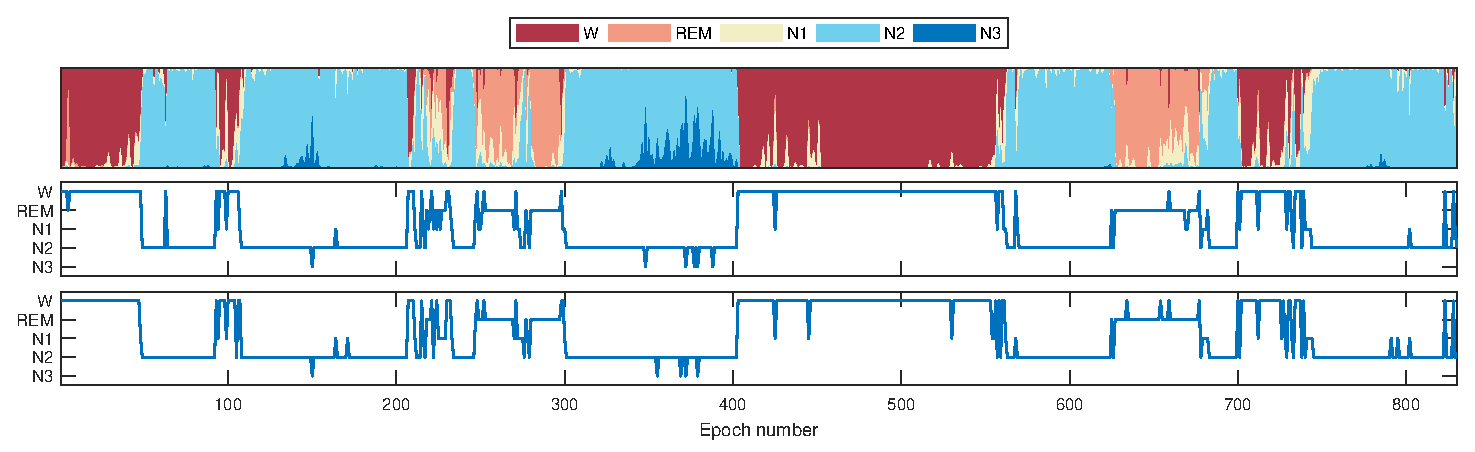
\includegraphics[width=\linewidth]{figures/paper-i/test_maxacc_id1627.eps}
    \caption[\acs{MASSC} hypnodensity example]{Top: hypnodensity graph of per-epoch probability distributions, middle: automatically scored hypnogram by applying~\cref{eq:argmax}. Bottom: manually scored hypnogram. Note the intrusions of \ac{N3} into \ac{N2} around epoch 150 and 370, and \ac{N1} into \ac{W} around 420.}
    \label{fig:slee-stages:hypnodensity}
\end{adjustwidth*}
\end{figure}

\begin{table}
    \small
    % increase table row spacing, adjust to taste
    % \renewcommand{\arraystretch}{1.3}
    \centering
    \begin{threeparttable}
    \caption[\acs{MASSC} train and validation performance, \acs{WSC}]{Averaged performance metrics for configurations.}% across train and eval subgroups.}
    \label{tab:sleep-stages:train_eval_performance}
    \begin{tabular}{@{}clccc@{}}
        \toprule
                              &          & \textbf{Baseline}          & \textbf{Weighted}          & \textbf{Balanced}          \\ \midrule
        \multirow{5}{*}{\textbf{Train}} & Acc, \%      & $ \mathbf{86.1 \pm 5.5} $ & $ 79.4 \pm 7.1 $ & $ 80.4 \pm 7.3 $ \\
                              & $\kappa$, \% & $ \mathbf{77.1 \pm 8.6} $ & $ 69.5 \pm 9.7 $ & $ 70.7 \pm 9.8 $ \\
                              & Pr, \%       & $ 87.1 \pm 4.9 $ & $ 88.7 \pm 4.1 $ & $ \mathbf{88.9 \pm 4.0} $ \\
                              & Re, \%       & $ \mathbf{86.1 \pm 5.5} $ & $ 79.4 \pm 7.1 $ & $ 80.4 \pm 7.3 $ \\
                              & F1, \%       & $ \mathbf{85.3 \pm 6.1} $ & $ 81.8 \pm 6.6 $ & $ 82.6 \pm 6.9 $ \\ \midrule
        \multirow{5}{*}{\textbf{Eval}}  & Acc, \%      & $ \mathbf{85.0 \pm 6.1} $ & $ 78.4 \pm 7.3 $ & $ 79.7 \pm 7.4 $ \\
                              & $\kappa$, \% & $ \mathbf{75.4 \pm 9.5} $ & $ 68.1 \pm 10.5 $ & $ 69.7 \pm 10.0 $ \\
                              & Pr, \%       & $ 86.3 \pm 5.3 $ & $ 87.8 \pm 4.8 $ & $ \mathbf{88.0 \pm 4.9} $ \\
                              & Re, \%       & $ \mathbf{85.0 \pm 6.1} $ & $ 78.4 \pm 7.3 $ & $ 79.7 \pm 7.4 $ \\
                              & F1, \%       & $ \mathbf{84.0 \pm 7.2} $ & $ 80.7 \pm 7.1 $ & $ 81.9 \pm 7.1 $ \\ \bottomrule
    \end{tabular}
    \begin{tablenotes}
    \item Metrics are shown as mean \(\pm\) standard deviations across each \ac{PSG}. Best performing model for each metric is shown in bold.
    \end{tablenotes}
    \end{threeparttable}
\end{table}

\begin{table}[tb]
    \small
    % increase table row spacing, adjust to taste
    % \renewcommand{\arraystretch}{1.3}
    \setlength{\tabcolsep}{4pt}
    \caption[\acs{MASSC} test group confusion matrix, \acs{WSC}]{Aggregated confusion matrix and stage-specific performance metrics in test subgroup.}
    \label{tab:sleep-stages:test_performance_aggregated}
    \centering
    \begin{threeparttable}
    \begin{tabular}{@{}llcccccccc@{}}
        \toprule
         & & \multicolumn{5}{c}{\textbf{Automatic}} & & & \\ \cline{2-7}
                 & \acs{W}     & \acs{W}   & \acs{N2}    & \acs{N3}   & \acs{REM}   & Pr, \% & Re, \% & F1, \% \\ \midrule
        \multirow{5}{*}{\textbf{Manual}} & \acs{W}        & 37980 & 1322 & 852   & 2    & 327   & 84.3    & 93.8    & 88.8    \\
         & \acs{W}       & 3922  & 8784 & 3545  & 0    & 2193  & 51.9    & 47.6    & 49.7    \\
         & \acs{N2}       & 1756  & 5136 & 99564 & 1091 & 991   & 88.6    & 91.7    & 90.2    \\
         & \acs{N3}       & 18    & 1    & 7932  & 4063 & 14    & 78.8    & 33.8    & 47.3    \\
         & \acs{REM}        & 1361  & 1680 & 465   & 0    & 23931 & 87.2    & 87.2    & 87.2    \\ \bottomrule
    \end{tabular}
    \begin{tablenotes}
        \small
        \item%
        \describe{W}; %
        \describe{N1}; %
        \describe{N2}; %
        \describe{N3}; %
        \describe{REM}.
    \end{tablenotes}
    \end{threeparttable}
\end{table}


Evaluating the baseline model on the test subgroup, only a slight drop in accuracy and $\kappa$ is observed, indicating that the model generalizes well, see~\cref{tab:sleep-stages:test_performance_aggregated} and~\cref{tab:sleep-stages:test_performance_average}.
The lowest sensitivity is obtained for \ac{N1} and \ac{N3}, which is in accordance with clinical experience reported in the literature~\cite{Younes2017, Rosenberg2013, Norman2000, Younes2016}.
N1 is a transitional stage between wakefulness, drowsiness and sleep often containing beta and alpha activity in epochs of low interscorer agreement, which explains the low predictive power in the confusion matrix.
The sleep continuum is also apparent in~\cref{fig:slee-stages:hypnodensity} which shows the manually and automatically scored hypnograms in the middle and bottom traces, and the hypnodensity graph in the top trace for a representative subject in the test subgroup.
The hypnodensity is a probabilistic representation of the hypnogram, which has found use in the detection of narcolepsy and Parkinson's disease~\cite{Koch2014, Christensen2014, Stephansen2018}.

Our baseline model attains favorable performance when comparing to the results reported for the raw waveform CNN model in~\cite{Biswal2017} with both higher accuracy and Cohen's kappa.
However, it should be stressed that~\cite{Biswal2017} only used \ac{EEG} channels from 9000 recordings, while our model uses both \ac{EEG}, \ac{EOG} and \ac{EMG} data, but only from 1850 recordings.
Furthermore, our baseline model performs only slightly worse compared to the best-performing model in~\cite{Biswal2017} without using any memory networks.
This indicates a performance gain by adding recurrent networks, such as long short-term memory cells, to our network.

A possible limiting factor to our model is the filter kernels.
The small filter sizes in block layers might not be able to accurately capture the physiological dynamics, but there are indications that many, smaller kernels are preferable to fewer, larger kernels when comparing model complexity versus computational costs~\cite{Szegedy2015}.

Future work will include adding more data to balance classes, and adding long short-term memory cells to the network in order to model temporal dynamics between epochs.
\begin{table}[tb]
    \small
    \centering
    \begin{threeparttable}
    \caption[MASSCv1 overall test performance, \acs{WSC}]{Performance across recordings in test subgroup.}
    \label{tab:sleep-stages:test_performance_average}
    \begin{tabular}{@{}ccccc@{}}
    \toprule
        \textbf{Accuracy}              & $\boldsymbol{\kappa}$         & \textbf{Pr}               & \textbf{Re}               & \textbf{F1}               \\ \midrule
        $ 84.1 \pm 6.9 $ & $ 0.746 \pm 0.099 $ & $ 85.7 \pm 6.1 $ & $ 84.1 \pm 6.9 $ & $ 83.1 \pm 7.6 $ \\ \bottomrule
    \end{tabular}
    \begin{tablenotes}
    \item Values are shown as mean \(\pm\) standard deviation across \acs{PSG}. Pr: precision; Re: recall.
    \end{tablenotes}
    \end{threeparttable}
\end{table}

\clearpage\section{Paper II: Automatic sleep stage classification with deep residual networks in a mixed-cohort setting}\label{sec:paperii}
\sectionmark{Olesen, Jennum, Mignot, \& Sorensen, 2020 (\textit{submitted)}}



\subsection{Cohort descriptions}
To investigate and conclude on generalizability of any machine learning or sleep stage classification model, multiple heterogenous datasets must be used for training, validation and testing purposes.
In this work, we collected datasets from five different sources, each dataset containing a diverse collection of subjects presenting with multiple disease phenotypes.
Details of the separate cohorts are shown in Table 1 along with reported \textit{p}-values highlighting cohort differences.
Each cohort was split into a training, validation and testing subset in proportions of 87.5\%, 2.5\% and 10\%, respectively, using random sampling without replacement among unique subjects, so that no subject is shared between subsets.
With these percentages, we maximize the number of PSGs available for training, while still reserving enough PSGs for validation and testing.
Collecting all the separate subsets across cohorts forms a training, validation, and testing partition, containing the respective subsets from all five cohorts. 

\subsubsection{Institute of Systems and Robotics, University of Coimbra Sleep Cohort (ISRUC)}
This cohort contains 126 recordings from 118 unique subjects recorded at the Sleep Medicine Centre of the Hospital of Coimbra University, Portugal, in the period 2009–2013~\cite{Khalighi2016}.
The cohort comprises three subgroups: subgroup I contains 100 PSGs of subjects with diagnosed sleep disorders, generally sleep apnea; subgroup II contains 16 recordings of eight subjects most of which are also diagnosed with sleep apnea; and subgroup III contains recordings from 10 subjects with no diagnosed sleep disorders.
All PSGs were recorded with the same recording hardware and software and each was scored by two technicians for sleep stages and sleep events according to the AASM guidelines.
ISRUC-Sleep is a freely accessible resource and all data and PSG files can be located at \url{https://sleeptight.isr.uc.pt/ISRUC_Sleep/}.

\subsubsection{The MrOS Sleep Study (MrOS)}
The MrOS sleep study is part of the larger Osteoporotic Fractures in Men Study, which aims to understand the relationships between sleep disorders, fractures, and vascular diseases in community-dwelling men~\cite{Blank2005, Orwoll2005, Blackwell2011}. 
It consists of 2907 in-home PSG recordings with an additional 1026 follow-up PSG studies from subjects recruited from six different clinical centers in the USA.
Each recording was annotated by an expert technician according to Rechtschaffen and Kales (R\&K) criteria for sleep staging~\cite{Rechtschaffen1968}.
For compatibility with AASM guidelines, we combined stages labeled S3 and S4 into N3. All data were accessed from the National Sleep Research Resource (NSRR) repository~\cite{Dean2016, Zhang2018}.

\subsubsection{The Sleep Heart Health Study (SHHS)}
The SHHS is a large, multi-center study on cardiovascular outcomes related to sleep disorders with a specific focus on sleep-disordered breathing~\cite{Redline1998, Quan1997}.
The cohort consists of 6441 subjects above 40 years old recruited between 1995 and 1998 undergoing in-home PSG (SHHS Visit 1) with subsequent follow-up PSG between 2001 and 2003 in 3295 subjects (SHHS Visit 2).
PSG recordings were annotated for sleep stages by trained and certified technicians according to R\&K rules.
From the original cohort we extracted 5793 PSGs and annotations from Visit 1, and 2651 from Visit 2.
We aggregated S3 and S4 stages into N3 similar to MrOS.
All data were accessed from NSRR repository.

\subsubsection{Wisconsin Sleep Cohort (WSC)}
WSC is a population-based study of sleep-disordered breathing in government workers in Wisconsin, USA that was initiated in 1988~\cite{Young1993, Young2008}.
In this work, we used 2412 PSGs from 1091 unique subjects in the WSC sample scored by expert technicians according to R\&K rules with subsequent merging of S3 and S4 into N3.

\subsubsection{Stanford Sleep Cohort (SSC)}
PSGs from this cohort originate from patients referred for sleep disorders evaluation and recorded at the Stanford Sleep Clinic since 1999.
The specific sample used in this study represents a small subset ($n=772$) of the whole cohort, which was selected and described in detail in previous studies scored according to R\&K or AASM guidelines according to prevailing standard at the time of evaluation~\cite{Andlauer2013, Moore2014}. 


\subsection{Methods}
\subsubsection{Data pipeline}
Electrophysiological signals corresponding to the minimum acceptable montage for sleep staging available across all cohorts were extracted for each PSG.
These included a central EEG (either C3 or C4 referenced to the contra-lateral mastoid), left and right EOG referenced to the contra-lateral mastoid, and a single submentalis EMG.
The choice between C3 and C4 was determined based on the lowest total signal energy across the entire duration of the PSG to avoid excessive signal popping.
Other methods to determine appropriate channels include algorithms based on shortest Mahalanobis distance to an already determined reference distribution~\cite{Stephansen2018}, but was not investigated in this study.
All signals were resampled to $f_s = \SI{128}{\hertz}$ using a polyphase filtering procedure irrespective of original sampling frequency, and subsequently filtered using a zero-phase approach with \nth{4} order Butterworth IIR filters (0.5 to 35 Hz band pass for EEG and EOG; 10 Hz high pass for EMG) in accordance with AASM filter specifications~\cite{Berry2020}.
Each signal was normalized to zero mean and unit variance to accommodate differences in recording equipment and baselines, and to compress the dynamic range into something easily trainable for the neural network architecture.
We denote by $C$ the number of input signals supplied to the neural network, where in this case $C=4$.

\subsubsection{Machine learning problem}
We designate by $\mathcal{X} \in \real^{C \times T}$ the set of \SI{30}{\second} input data segments with $S$ input channels and segment length $T$, and the corresponding sleep stage classifications by $\mathcal{Y} = \lbrace y \in \real_{+}^{K} \mid \sum_i y_i = 1 \rbrace$, where $K = 5$ corresponds to the five sleep stages.
Thus, $y$ is a probability simplex, which maps to the ordered set $\mathcal{S} = \lbrace \wake, \nI, \nII, \nIII, \rem \rbrace$ by the argmax function such that $\argmax{y : \mathcal{Y} \to \mathcal{S}}$.
Furthermore, as we are potentially interested in classifying multiple sleep stages at once, we extend the problem of classifying a single sleep stage given $x \in \mathcal{X}$ to a sequence-to-sequence problem, in which we desire to learn a differentiable function representation $\Phi$, that maps a sequence of \SI{30}{\second} epochs $\mathbf{x} \in \real^{C \times \alpha T}$ to their corresponding label probabilities $\mathbf{y} \in \real^{K \times \alpha}$, where $\alpha$ is a parameter that controls the sequence length. 
For example, if $\alpha=8$, the sequence $\mathbf{x}$ contains \SI{4}{\minute} of successive PSG data described by 8 epochs of length \SI{30}{\second}.
Furthermore, we denote by $\llbracket a, b \rrbracket$ the set of integers from $a$ to $b$, i.e. $\llbracket a, b \rrbracket = \lbrace n \in \mathbb{N} \mid a \leq n \leq b \rbrace$, and by $\llbracket N \rrbracket$ the shorthand form of $\llbracket 1, N \rrbracket$.

\subsubsection{Network architecture}
\begin{figure}
    \includegraphics[width=\textwidth+\marginparwidth+\marginparsep]{figures/paper-ii/figure_01_a-b.pdf}
    \caption{Caption}
    \label{fig:paper-ii-figure1}
\end{figure}
As the representation of $\Phi$, we adapted and extended a previously published neural network architecture for automatic sleep stage classification, which was based on a variant of the ResNet-50 architecture commonly used for two-dimensional image classification tasks, but adapted and re-trained from scratch for the specific use-case of one-dimensional, time-dependent signals in the PSG~\cite{Olesen2018c}.
This network has the advantage that it does not require any manual feature engineering and extraction compared to previous state of the art sleep stage classification models~\cite{Stephansen2018}.
An overview of the proposed network architecture is provided graphically in Figure 1 and Table 2.
Briefly, the architecture consists of four modules:
\begin{enumerate}
    \item an initial mixing module 
    \begin{equation}
        \varphi_{\mathrm{mix}} : \real^{1 \times C \times T} \to \real^{C \times 1 \times T},
    \end{equation}%$\varphi_{\mathrm{mix}} : \real^{1 \times C \times T} \to \real^{C \times 1 \times T} $,
	\item a feature extraction module
	\begin{equation}
	    \varphi_{\mathrm{feat}} : \real^{C \times 1 \times T} \to \real^{f_0 2^{R+1} \times 1 \times T/2^R},
	\end{equation}
	\item a temporal processing module
	\begin{equation}
	    \varphi_{\mathrm{temp}}     : \real^{f_0 2^{R+1} \times 1 \times T/2^R} \to \real^{2n_h \times T/2^R}, \, \text{and}
	\end{equation} %$\varphi_{\mathrm{temp}}     : \real^{f_0 2^{R+1} \times 1 \times T/2^R} \to \real^{2n_h \times T/2^R} $, and
	\item a classification module
	\begin{equation}
	    \varphi_{\mathrm{clf}} : \real^{2n_h \times T/2^R} \to \real^{K \times T/2^R}.
	\end{equation}%$\varphi_{\mathrm{clf}} : \real^{2n_h \times T/2^R} \to \real^{K \times T/2^R}$.
\end{enumerate}
Thus, we obtain a differentiable representation of the function  $\Phi$ as
\begin{align}
\begin{split}
    &\Phi : \real^{C \times K} \to \real^{K \times T/2^R} \\
    &\Phi\left(\mathbf{x}\right) = \varphi_{\mathrm{clf}} \left( \varphi_{\mathrm{temp}} \left( \varphi_{\mathrm{feat}} \left( \varphi_{\mathrm{mix}} \left( \mathbf{x} \right) \right) \right) \right).
\end{split}
\end{align}
The output of this function is the matrix $\mathbf{y} \in \real^{K \times T/2^R}$ containing sleep stage probabilities in the sequence of PSG data evaluated every second.

\paragraph{Mixing module}
The raw input data is input to this module, which encourages non-linear channel mixing similar to what has been proposed in recent literature~\cite{Chambon2018c, Chambon2018b, Chambon2019, Olesen2019}.
The module is realized using a single 2D convolutional operation outputting $C$ feature maps computed using single-strided $(C \times 1)$ kernels followed by rectified linear unit (ReLU) activations.

\paragraph{Feature extraction (residual network) module}
This is comprised of a succession of $R$ residual blocks (see Figure 1)\todo{fix}, which are responsible for the bulk feature extraction from the channel-mixed data.
Each residual block is realized using bottlenecks of first a $1\times 1$ convolution to reduce the number of feature maps, then a $1\times 3$ convolution, and lastly a $1 \times 1$ convolution to finally increase the number of feature maps. 
Each convolution operation is followed by a batch normalization~\cite{Ioffe2015} and ReLU activation except after the last convolutional layer, where shortcut projections are added before the activation~\cite{He2016b}.
This type of block structure enables the design and training of very deep networks without the risk of vanishing gradients due to the projection shortcuts~\cite{He2016}.

\paragraph{Temporal processing module}
This module is realized by a bidirectional gated recurrent unit (GRU)~\cite{Cho}45 in order to accommodate temporal dependencies in the PSG.
The GRU runs through the temporal dimension of the output from $\varphi_{\mathrm{feat}}$ of $T/2^R$ time steps each containing $f_0 2^{R+1}$ feature maps and outputs $n_h$ new features in each direction for each time step.
By running both forward and backward, we can accommodate that technicians base their scoring on looking backwards as well as ahead in time in each time segment (typically 30 s).

\paragraph{Classification module}
The final module in the architecture performs actual classification based on the forward and backward features for each time step outputted from $\varphi_{\mathrm{temp}}$.
It is realized by a single convolutional operation with a subsequent softmax activation to compute a probability distribution over the $K$ sleep stage classes, such that the probability of sleep stage $i$ at time step $n$ is given by $y_i^{(n)} = \frac{\exp{a_i}}{\sum_k{\exp{a_k}}}$)), where $a_i \in \mathbf{a}$ is the activation of the last layer in the network and $k=\llbracket K \rrbracket$.


\subsubsection{Loss function specification}
The network was trained end-to-end with respect to a loss function, that takes the output probabilities from the network $y = \Phi\left( \mathbf{x} \right)$ and calculates the loss as
\begin{align}
\begin{split}\label{eq:loss-paperII}
    \mathcal{L}\left( \mathbf{y} \right) &= - \sum_{n=1}^{30/\tau}\sum_{k=1}^{K} t_k^{(n)}\log{\left( \tilde{y}^{(n)}_k \right)}, \\
    \tilde{y}^{(n)}_k &= \frac{1}{\tau} \sum_{i=\tau \left( j - 1 \right) + 1}^{\tau n} y_k^{(i)},
\end{split}
\end{align}
which is the cross-entropy between successive time-averaged classifications parameterized by the number of successive one-second predictions $\tau$, and the ground truth labels $t$ broadcasted to $\frac{30}{\tau}$ labels per \SI{30}{\second} segment.
This way, we can acquire predictions every second, that can be combined in time at intervals given by $\tau$.

\subsubsection{Experimental setups}
We set up three different experiments in this study.
\begin{enumerate}
    \item We wished to investigate the effect of increasing the complexity of the recurrent module by varying the number of units $n_h$ in the module $\varphi_{\mathrm{temp}}$ in the space $n_h=2^k, k \in \llbracket 6, 11 \rrbracket$.
    We hypothesize that there exists a sweet-spot in the number of hidden units that balances computational complexity with classification performance, i.e. classifying a sequence of sleep stage labels given a corresponding sequence of outputs from $\varphi_{\mathrm{feat}}$.
    The results of this experiment were furthermore used to determine parameters for models in subsequent experiments.
    \item Since we have several cohorts at our disposition of both clinical and research origin, we can investigate the compatibility and inherent generalizability of the different cohorts in two ways: 1) we set aside a single cohort for testing, while we train the models on the remaining four (leave-one-cohort-out, LOCO training); and 2) we train on a single cohort, while we set aside the remaining four for testing (leave-one-cohort-in, LOCI training).
    \item Generalizability can also be investigated in another way, which can answer the question of how many data sources is necessary.
    We trained models with all possible 2-, 3-, and 4-combinations of cohorts, i.e. one run trained on ISRUC and MrOS training data, another run with ISRUC and SHHS train data, a third with ISRUC and SSC, etc., with all runs subjected to subsequent evaluation on the test partition. 
    \item Previous studies have already investigated the performance of automatic sleep staging algorithms using shallow machine learning models.
    At the time of writing however, none have investigated the effect of available training data for deep learning models at this magnitude (up to tens of thousands).
    We therefore trained models on 0.25\%, 0.5\%, 1\%, 5\%, 10\%, 25\%, 50\%, 75\% and 100\% of the data available for training.
    Specifically, some of these fractions of the total number of PSGs correspond roughly to the number of PSGs in the training partitions in each cohort, allowing for direct comparisons between training a model with mixed- and single-cohort training data.
\end{enumerate}

Common for all experiments were the default parameter values $C=4$, $f_s=\SI{128}{\hertz}$, $T=\tau f_s$, $K=5$, $R=7$, and $f_0=4$ for the number of input channels, sampling frequency, the sequence length, the number of sleep stages, the number of consecutive residual blocks, and the base filter kernel size, respectively.
All models were trained for 50 epochs (passes through the training partition) and the model with the highest Cohen’s kappa value on the validation partition was subsequently selected for testing.
All models were trained end-to-end with backpropagation using the Adam optimizer~\cite{Kingma2015} with a learning rate of $10^{-4}$, $\beta_1=0.9$, and $\beta_2=0.999$ to minimize the loss function specified by \cref{eq:loss-paperII}. 
All network weights and bias terms were initialized using the uniform Glorot initialization scheme~\cite{Glorot2010}. 

\subsubsection{Performance metrics and model evaluation}
For each experiment we evaluated model performance using the overall accuracy (Acc) and \cohen in order to take account the possibility of chance agreement between the model and the gold standard.
Given a confusion matrix $\mathbf{C}$ with element $c_{ij}$ being the number of epochs belonging to sleep stage $i$ but classified to be in sleep stage $j$, we define the overall accuracy for a given model as
\begin{equation}
    \text{Acc} = \frac{\sum_{i=j}c_{ij}}{\sum_{i,j}c_{ij}},
\end{equation}
\ie the sum of the trace of $\mathbf{C}$ divided by the total count.
The \cohen metric is defined as
\begin{equation}
    \kappa = \frac{p_o - p_e}{1 - p_e},
\end{equation}
where $p_o = \text{Acc}$ is the observed agreement (\ie accuracy) and $p_e$ is the expected chance agreement, which can be reformulated in terms of the outer product between the row and column sums (class-specific recall and precision) of $\mathbf{C}$.


\subsection{Results}

\subsubsection{Temporal context impact on model performance}
\begin{figure}
    \centering
    \includegraphics[width=\columnwidth]{figures/paper-ii/figure_02_a-c.pdf}
    \caption[MASSCv2 temporal context]{Caption}
    \label{fig:paper-ii-figure2}
\end{figure}
In~\cref{fig:paper-ii-figure2} we show how the model performance depends on the temporal context and complexity of the temporal processing module, when evaluating the model on the validation partition.
Results are further detailed in Table S1\todo{supplementary tables???}.
Specifically, we observe a drastic change in \cohen just by introducing a simple recurrent unit into the network as shown in~\cref{fig:paper-ii-figure2}a, where \cohen increases from \ci{0.645}{0.126}{0.633}{0.657} at $n_h=0$ to \ci{0.720}{0.120}{0.709}{0.731} at $n_h=64$. 
We did not observe any major changes when increasing the number of hidden units beyond $n_h=64$, although we did see a maximum \cohen of \ci{0.734}{0.111}{0.723}{0.744} at $n_h=1024$, which is shown in the inset in~\cref{fig:paper-ii-figure2}a. 
We observed a general increase in \cohen when classifying longer sequences than \SI{2}{\minute} (\ci{0.726}{0.114}{0.715}{0.737}), but did not see any major differences when classifying over more than \SI{3}{\minute} sequences (\ci{0.733}{0.123}{0.721}{0.7444}).
Subsequent models were fixed with $n_h=1024$ corresponding to a sequence length of \SI{5}{\minute}.

\subsubsection{Model classifications converge to 30 s predictions given sufficient training data}
Furthermore, we analyzed the classification performance of the model given a specific sequence length by looking at the average prediction accuracy across all \SI{5}{\minute} sequences in all subject PSGs in the test partition, similar to what~\citeauthor{Brink-Kjaer2019} has shown previously~\cite{Brink-Kjaer2019}.
In~\cref{fig:paper-ii-figure2}c, we show how the average classification accuracy in a \SI{5}{\minute} sequence both depends on the amount of data and the frequency of evaluating the model output, \ie every \SI{1}{\second} or across \SI{30}{\second}.
The average classification accuracy was found to be slightly lower in the beginning of each \SI{5}{\minute} sequence, both when training a model with less (500 training subjects) and more (\SI{75}{\percent} of total training subjects).
Interestingly, when training with less data, we also observed a lower accuracy in the beginning and end of each \SI{30}{\second} segment relative to the accuracy in the middle section, which was not the case when training with more data.

\subsubsection{Choice of cohort impacts classification performance on test set}
\begin{figure}
    \centering
    \includegraphics[width=\columnwidth]{figures/paper-ii/figure_03_a-b.pdf}
    \caption[MASSCv2 LOCI and LOCO performance]{Caption}
    \label{fig:paper-ii-figure3}
\end{figure}
In~\cref{fig:paper-ii-figure3} we show how training on different cohorts yield differing results in subsequent testing performance, here expressed in heatmaps as both overall accuracy (\cref{fig:paper-ii-figure3}a), and \cohen (\cref{fig:paper-ii-figure3}b) averaged across all $N=1584$ subject PSGs in the test partition.
The first two columns show the performance on the cohort on the \textit{x}-axis, when training on the specific cohort on the \textit{y}-axis.
Since the training subset in ISRUC is small compared to the other cohorts, we trained the models in the left-most column with weight decay of $10^{-4}$ to compensate for the risk of overfitting, however, by comparing the left and middle columns, we did not observe any specific gain in classification performance by doing so.
The right-most column shows the test performance for each cohort, when excluding that cohort from training.
We observe a significant spread in classification accuracy across the different cohorts with prediction on ISRUC being poorest, while prediction on MrOS data being best.
Further details can be found in Table S2\todo{Supp. tables?}.

\subsubsection{More data is good, diverse data is better}
\begin{figure}
    \centering
    \includegraphics[width=\columnwidth]{figures/paper-ii/figure_04_a-b.pdf}
    \caption{Caption}
    \label{fig:paper-ii-figure4}
\end{figure}
We observed a general increase in classification performance both in terms of overall accuracy and \cohen, when including more data in the model training phase in both the mixed- and single-cohort setting (\cref{fig:paper-ii-figure4}a, Table S3\todo{Suppl. table}).
Classification performance was consistently lower in the single-cohort setting compared to the corresponding mixed-cohort setting. 
Interestingly, we found that training a model with just \SI{0.25}{\percent} of mixed-cohort training data still achieved an acceptable accuracy comparable to training a model with only SHHS data, while using all available training data increased that performance by almost 10 percentage points.
Furthermore, we observed that the model trained with \SI{100}{\percent} of the training partition reached a state-of-the-art level of performance with an overall accuracy of \ci{0.869}{0.064}{0.865}{0.872} and \cohen of \ci{0.799}{0.098}{0.794}{0.804} (see Table S3\todo{Suppl. table}).
The model furthermore performs well with respect to classifying individual sleep stages as shown in the confusion matrix in~\cref{fig:paper-ii-figure4}b.
However, the model still has difficulties classifying and distinguishing between certain sleep stages, especially between N2, N1, and N3; and W, N2, and N1.

\subsubsection{Increasing the number of data sources improves classification performance}
\begin{figure}
    \centering
    \includegraphics[width=0.75\columnwidth]{figures/paper-ii/figure_05.pdf}
    \caption{Caption}
    \label{fig:paper-ii-figure5}
\end{figure}
On average, we saw an increase in overall accuracy, when increasing the number of cohorts from 2 to 4 using 500 PSGs in each configuration, see~\cref{fig:paper-ii-figure5} and Table S4\todo{Suppl. table}.
Specifically, we found that the average overall accuracy increased from \ci{0.788}{0.102}{0.787}{0.790} in the 2-cohort configuration to \ci{0.808}{0.092}{0.807}{0.810} and \ci{0.821}{0.085}{0.819}{0.823} in the 3- and 4-cohort configurations, respectively.

\subsection{Discussion}
In this work, we present an end-to-end deep learning-based model for fully automatic micro- and macro-sleep stage classification. 
Using all of the available data sources for training our model, we reached an overall accuracy on test partition of \ci{0.869}{0.064}{0.865}{0.872}, and a \cohen of \ci{0.799}{0.098}{0.794}{0.804}, which is in the very high end of the substantial agreement category for observer agreement51.
We found that individual cohorts exhibit major differences in overall accuracy and \cohen when subjected to both training and testing conditions and specifically, we found that average performance on the test partition in the LOCI configurations varied significantly from \ci{0.676}{0.124}{0.670}{0.682} when training on ISRUC, to \ci{0.837}{0.084}{0.833}{0.841} when training on SHHS.
Each individual cohort also showed large deviations in predictive performance when tested on the other cohorts.
For example, when conditioned on SHHS data, the lowest average accuracy was 0.721 on SSC test data compared to the highest at 0.872 on SHHS test data, while conditioning on SSC training data, the lowest average accuracy was 0.704 on ISRUC test data compared to 0.824 on WSC test data.
Classification performance was generally higher on the test set when using the LOCO configuration, except for SHHS (higher in LOCI) and SSC (no difference).
We also found that having data from multiple sources always resulted in better-performing models compared to training on single cohorts.
Increasing the number of data sources increased classification performance, although this was non-significant.
In the design of the model, we observed that model performance was enhanced by the addition of the recurrent module (bGRU), a phenomenon likely reflecting the fact that sleep stage scoring at a specific time in one subject can be influenced by signal content (frequency, amplitude, presence of micro-events) at later time steps.
However, the complexity of the module given by the number of hidden units did not affect performance.
In all our experiments, we also evaluated the performance of the model every 1 s compared to the performance evaluated every 30 s and found them to be similar, which indicates the model is stable in classification in periods corresponding to an epoch of data.

Only a handful of studies have previously reported results when using multiple cohorts~\cite{Stephansen2018, Biswal2018a, Patanaik2018}.
Some authors have reported a drop from 81.9\% to 77.7\% when training on the Massachusetts General Hospital cohort (MGH) and testing on MGH and SHHS, respectively~\cite{Biswal2018a}, while others have shown significant drops from 89.8\% to 81.4\% and 72.1\% on two separate hold-out sets from Singapore and USA~\cite{Patanaik2018}.
We also observed similar trends in our LOCI and LOCO experiments, where excluding the training subset of a cohort from the training partition resulted in a significant drop in performance on the respective test subset from that cohort.
A benefit of our LOCI and LOCO experiments is the possibility for direct benchmarking against previous publications using specific cohorts in their experiments.
For example, we obtain an accuracy of 0.805 in the LOCO-SHHS training-testing case compared to 0.777 previously reported by~\citeauthor{Biswal2018a}~\cite{Biswal2018a}, both of which reflect classification performance when SHHS had not been used for training; and an accuracy of 0.865 in the LOCI-WSC case compared to 0.841 reported by \citeauthor{Olesen2018c}~\cite{Olesen2018c}, where both have been using a subset of WSC for training the model. 
Interestingly, we obtained the same level of performance on the SHHS data in our LOCI experiment as reported by \citeauthor{Sors2018} (87\% accuracy, 81\% \cohen) even though they only used single-EEG for their experiments~\cite{Sors2018}.
Other works that have investigated single- vs. multi-channel models for automatic sleep stage classification have found that models generally benefit from having more channels available for training~\cite{Chambon2018c, Biswal2018a, Phan2019a}.
It may be that some cohorts share different characteristics that makes them more suitable for single- or multi-channel models, but this is speculative and would need to be verified in subsequent studies.

We only optimized our network architecture with respect to the temporal processing module and therefore cannot assess what impact different design choices for the other modules would have had on final performance.
For example, the EMG signal has different statistical properties and spectral content, and separate, parallel architectures for EMG and EEG/EOG feature extraction may be warranted, as proposed by others~\cite{Chambon2018c, Stephansen2018}.
Other studies have however shown equal performance in large cohorts using a similar channel mixing approach as proposed here~\cite{Olesen2018c}.
Another limitation is found in our training runs, as we did not consider balancing our data with respect to the proportion of sleep stages, which may or may not have had impact on overall performance.
It is well established that there is significant variation in scoring and validation of N1/REM and N2/N3~\cite{Younes2016, Younes2018, Norman2000}, which challenges the training for any classification algorithm.
Some researchers have experimented balancing the cost of misclassifying sleep stages by weighting them by their inverse frequency of occurrence and found no significant improvement~\cite{Olesen2018c, Sors2018}, while others have experimented with balancing the sleep stage frequencies in each batch of data input to the neural network model~\cite{Chambon2018c}, but more rigorous research in resampling or over/under-sampling techniques is warranted in this regard.
We ultimately decided against experimenting with balancing our sleep stages in each batch, as we prioritized flexibility with regards to the length of input sequences fed to the network.
All our models ran through at least 50 epochs of training (passes through the training partition), which might have induced a bias in the configurations with larger cohorts.
For example, one pass through the training partition in the LOCI-ISRUC case corresponds to much less data than one pass through the LOCI-SHHS case.
However, since we selected the best performing model based on \cohen across all 50 epochs, we have allowed for more effective training in cases with less available training data.
We observed that models using less data in the training partition generally had to run for longer time (\ie more epochs) before converging.

In future studies on automatic sleep stage classification algorithms, we strongly recommend researchers to test and report results on not just hold-out test partitions, but also on cohorts completely unseen by the model both during training and testing/validation.
Our experiments indicate that even though good performance can be achieved on hold-out data using a single cohort, this does not necessarily translate into good generalization performance.
Such approach requires availability of many publicly available, high-quality, well-documented databases with easily accessible PSG data, associated annotations and related patient information.
In this regard, websites such as the NSRR, which contains several large databases with clinical data as well as PSG and annotation data in a standardized format~\cite{Dean2016,Zhang2018}, are an invaluable resource for researchers. 
We also propose that the sleep science community establishes a common reference dataset on which researchers in machine learning can benchmark their models, similar to what the computer vision and general machine learning community has done with the ImageNet Large Scale Visual Recognition Challenge (ILSVRC)~\cite{Russakovsky2015}, an annual competition in which researchers submit their models to test in various competitions.

In summary, we have developed an automatic sleep stage classification algorithm based on deep learning, that can accurately classify sleep stages at a flexible resolution with a state-of-the-art classification performance of 87\% accuracy on a test set of 1584 PSGs.
We trained and tested our model using five cohorts with varying numbers of PSGs covering multiple phenotypes with specific focus on how well cohorts can generalize to each other.
We found that different cohorts generalize very differently both in intra- and inter-cohort settings (LOCI vs. LOCO experiments).
Furthermore, we also found that having more data sources significantly improve classification performance and generalizability to the extent that even just a small number of training PSGs can reach high classification performance by including many different sources.
To our knowledge, this is one of the largest, if not the largest, study on automatic sleep stage classification in terms of PSG volume, diversity, and performance.

\clearpage\section{Paper III: Neural network analysis of sleep stages enables efficient diagnosis of narcolepsy}\label{sec:paperiii}
\sectionmark{Stephansen \& Olesen, \textit{et al.}, 2018}

\subsection{Materials \& Methods}
\begin{figure}[t]
    \myfloatalign   
    \subfloat[]
    {\includegraphics[width=\textwidth]{figures/paper-iii/Figure_5a.png}}  \\
    \subfloat[]
    {\includegraphics[width=\textwidth]{figures/paper-iii/Figure_5b.png}}
    \caption[STAGES model for sleep staging]{Overview of STAGES model for sleep stage classification. (a) Pre-processing steps taken to achieve the format of data as it is used in the neural networks. One of the 5 channels is first high-pass filtered with a cut-off at 0.2 Hz, then low-pass filtered with a cut-off at 49 Hz followed by a re-sampling to 100 Hz to ensure data homogeneity. In the case of EEG signals, a channel selection is employed to choose the channel with the least noise. The data are then encoded using either the CC or the octave encoding. (b) Steps taken to produce and test the automatic scoring algorithm. A part of the SSC10, 32 and WSC32, 33 is randomly selected, as described in~\cref{tab:paperiii-table01}. These data are then segmented in 5 min segments and scrambled with segments from other subjects to increase batch similarity during training. A neural network is then trained until convergence (evaluated using a separate validation sample). Once trained, the networks are tested on a separate part of the SSC and WSC along with data from the IS-RC31 and KHC10, 34.}
    \label{fig:paperiii-figure05}
\end{figure}
\subsubsection{Datasets}
The success of machine learning depends on the size and quality of the data on which the model is trained and evaluated~\cite{Banko2001, Shotton2011}.
We used a large dataset comprised of several thousand sleep studies to train, validate, and test/replicate our models.
To ensure significant heterogeneity, data came from 10 different cohorts recorded at 12 sleep centers across 3 continents: SSC~\cite{Andlauer2013, Moore2014}, WSC~\cite{Moore2014, Young2009a}, IS-RC~\cite{Kuna2013}, JCTS~\cite{InternationalXyremStudyGroup2005}, KHC~\cite{Hong2006}, AHC~\cite{Frauscher2013}, IHC~\cite{Pizza2015}, DHC~\cite{Christensen2017}, FHC, and CNC~\cite{Andlauer2012}.
Institutional Review Boards approved the study and informed consent was obtained from all participants.
Technicians trained in sleep scoring manually labeled all sleep studies.
Figure 5 a, b, and c summarize the overall design of the study for sleep stage scoring and narcolepsy biomarker development.
\Cref{tab:paperiii-table01} provides a summary of the size of each cohort and how it was used.
In the narcolepsy biomarker aspect of the study, PSGs from T1N and other patients were split across most datasets to ensure heterogeneity in both the training and testing dataset.
For this analysis, a few recordings with poor quality sleep studies, i.e. missing critical channels, with additional sensors or with a too short sleep duration ($\leq$ 2 hours) were excluded.
A “never seen” subset cohort that included French and Chinese subjects (FHC and CNC) was also tested.
Below is a brief description of each dataset.

\paragraph{Population-based Wisconsin Sleep Cohort}
This cohort is a longitudinal study of state agency employees aged 37 - 82 years from Wisconsin, and approximates a population-based sample (see~\cref{tab:paperiii-table01} for age at study) and are generally more overweight33.
The study is ongoing, and dates to 1988.
2167 PSGs in 1086 subjects were used for training while 286 randomly selected PSGs were used for validation testing of the sleep stage-scoring algorithm and narcolepsy biomarker training.
Approximately 25\% of the population have an Apnea Hypopnea Index (AHI) above 15/hour and 40\% have a PLMI above 15/hr.
A detailed description of the sample can be found in Young33 and Moore et al.32.
The sample does not contain any T1N patients, and the three subjects with possible T1N were removed54.

\paragraph{Patient-based Stanford Sleep Cohort}
PSGs from this cohort were recorded at the Stanford Sleep Clinic dating back to 1999, and represent sleep disorder patients aged 18-91 visiting the clinic (see~\cref{tab:paperiii-table01} for age at study).
The cohort contains thousands of PSG recordings, but for this study we used 894 diagnostic (no positive airway pressure (PAP)) recordings in independent patients that have been used in prior studies30.
This subset contains patients with a range of different diagnoses including: sleep disordered breathing (607), insomnia (141), REM sleep behavior disorder (4), restless legs syndrome (23), T1N (25), delayed sleep phase syndrome (14), and other conditions (39).
Description of the subsample can be found in Andlauer et al.10 and Moore et al.32.
Approximately 30\% of subjects have an AHI above 15/hour, or a PLMI above 15/hour.
617 randomly selected subjects were used for training the neural networks while 277 randomly selected PSGs were kept for validation testing of the sleep stage scoring algorithm.
These 277 subjects were also used for training the narcolepsy biomarker algorithm.
The sample contains PSGs of 25 independent untreated subjects with T1N (12 with low CSF hypocretin-1, the others with clear cataplexy).
26 subjects were removed from the study—4 due to poor data quality, and the rest because of medication use.

\paragraph{Patient-based Korean Hypersomnia Cohort}
The Korean Hypersomnia Cohort is a high pretest probability sample for narcolepsy.
It includes 160 patients with a primary complaint of excessive daytime sleepiness (see~\cref{tab:paperiii-table01} for age at study).
These PSGs were used for testing the sleep scoring algorithm and for training the narcolepsy biomarker algorithm.
No data was used for training the sleep-scoring algorithm.
Detailed description of the sample can be found in Hong et al.34 and Andlauer et al.10
The sample contains PSGs of 66 independent untreated subjects with T1N and clear cataplexy.
Two subjects were removed from the narcolepsy biomarker study because of poor data quality.

\paragraph{Patient-based Austrian Hypersomnia Cohort}
Patients in this cohort were examined at the Innsbruck Medical University in Austria as described in Frauscher et al.35.
The AHC contains 118 PSGs in 86 high pretest probability patients for narcolepsy (see~\cref{tab:paperiii-table01} for details).
42 patients (81 studies) are clear T1N with cataplexy cases, with all but 3 having a positive MSLT (these three subjects had a mean sleep latency (MSL)>8 minutes but multiple SOREMPs).
The rest of the sample has idiopathic hypersomnia and type 2 narcolepsy.
Four patients have an AHI>15/hour and 25 had a PLMI>15/hour.
Almost all subjects had two sleep recordings performed, which were kept together such that no two recordings from the same subject were split between training and testing partitions.

\paragraph{Patient-based Inter-scorer Reliability Cohort}
As Rosenberg et al.16 have shown, variation between individual scorers can sometimes be large, leading to an imprecise gold standard.
To quantify this, and to establish a more accurate gold standard, 10 scorers from five different institutions, University of Pennsylvania, St. Luke’s Hospital, University of Wisconsin at Madison, Harvard University, and Stanford University, analyzed the same 70 full night PSGs.
For this study, scoring data from University of Pennsylvania, St. Luke’s and Stanford were used.
All subjects are female (see~\cref{tab:paperiii-table01} for details).
This allowed for a much more precise gold standard, and the inter-scorer reliability could be quantified for a dataset, which could also be examined by automatic scoring algorithms.
Detailed description of the sample can be found in Kuna et al.31 and Malhotra6.
The sample does not contain any T1N patients.

\paragraph{The Jazz Clinical Trial Sample}
This sample includes seven baseline sleep PSGs from five sites taken from a clinical trial study of sodium oxybate in narcolepsy (SXB15 with 45 sites in Canada, USA, and Switzerland) conducted by Orphan Medical, now named Jazz Pharmaceuticals.
The few patients included are those with clear and frequent cataplexy (a requirement of the trial) that had no stimulant or antidepressant treatment at baseline43.
All 7 subjects in this sample were used exclusively for training the narcolepsy biomarker algorithm.

\paragraph{Patient-based Italian Hypersomnia Cohort}
Patients in this high pretest probability cohort (see~\cref{tab:paperiii-table01} for demographics) were examined at the IRCCS, Istituto delle Scienze Neurologiche ASL di Bologna in Italy as described in Pizza et al.41.
The IHC contains 70 \ntI patients (\SI{58}{\percent} male, \plusminus{29.5}{1.9} years old), with either documented low CSF hypocretin levels (59 cases, all but 2 HLA DQB1*06:02 positive), or clear cataplexy, positive MSLTs and HLA positivity (11 subjects).
As non-\ntI cases with unexplained daytime somnolence, the cohort includes 77 other patients: 19 with idiopathic hypersomnia, 7 with type 2 narcolepsy and normal CSF hypocretin-1, 48 with a subjective complaint of excessive daytime sleepiness not confirmed by MSLT, and 3 with secondary hypersomnia.
Subjects in this cohort were used for training (n=87) and testing (n=61) the narcolepsy biomarker algorithm. 

\paragraph{Patient-based Danish Hypersomnia Cohort}
Patients in this cohort were examined at the Rigshospitalet, Glostrup, Denmark as described in Christensen et al53.
The DHC contains 79 PSGs in controls and patients (see~\cref{tab:paperiii-table01} for details).
Based on PSG, multiple sleep latency test and cerebrospinal fluid hypocretin-1 measures, the cohort includes healthy controls (19 subjects), patients with other sleep disorders and excessive daytime sleepiness (20 patients with CSF hypocretin-1 $\geq$ 110 pg/ml), narcolepsy type 2 (22 patients with CSF hypocretin-1 $\geq$ 110 pg/ml), and T1N (28 patients with CSF hypocretin 1 $\leq$ 110 pg/ml).
All 79 subjects in this cohort were used exclusively for training the narcolepsy biomarker algorithm.

\paragraph{Patient-based French Hypersomnia Cohort}
This cohort consists of 122 individual PSGs recorded at the Sleep-Wake Disorders Center, Department of Neurology, Gui-de-Chauliac Hospital, CHU Montpellier, France (see~\cref{tab:paperiii-table01} for demographics).
The FHC contains 63 subjects with T1N (all but two tested with CSF hypocretin-1 $\leq$ 110 pg/ml, five below 18 years old, 55 tested for HLA, all positive for HLA DQB1*06:02) and 22 narcolepsy type 2 (19 with CSF hypocretin-1 > 200 pg/ml, and three subjects with CSF hypocretin-1 between 110 and 200 pg/ml, three HLA positive).
The remaining 36 subjects are controls (15 tested for HLA, two with DQB1*06:02) without other symptoms of hypersomnia.
The FHC was used as data for the replication study of the narcolepsy biomarker algorithm.

\paragraph{Patient-based Chinese Narcolepsy Cohort}
This cohort contains 199 individual PSGs recorded (see~\cref{tab:paperiii-table01} for demographics).
The CNC contains 67 subjects diagnosed with T1N exhibiting clear-cut cataplexy (55 tested HLA DQB1*06:02 positive), while the remaining 132 subjects are randomly selected population controls (15 HLA DQB1*06:02 positive, 34 HLA negative, remaining unknown) 12.
Together with the FHC, the CNC was used as data for the replication study of the narcolepsy biomarker algorithm.

\paragraph{American Academy of Sleep Medicine Sleep Study}
The AASM ISR dataset is composed of a single control sleep study of 150 30 sec epochs that was scored by \plusminus{5234}{14} experienced sleep technologists for quality control purposes.
Design of this dataset is described in Rosenberg et al.16.

\subsubsection{Data labels, scoring and fuzzy logic}
Sleep stages were scored by PSG-trained technicians using established scoring rules, as described in the AASM Scoring Manual7.
In doing so, technicians assign each epoch with a discrete value.
With a probabilistic model, like the one proposed in this study, a relationship to one of the fuzzy sets is inferred based on thousands of training examples labeled by many different scoring-technicians. 

The hypnodensity graph refers to the probability distribution over each possible stage for each epoch, as seen in Figure 2 a and b.
This allows more information to be conveyed, since every epoch of sleep within the same stage is not identical. For comparison with the gold standard, however, a discrete value must be assigned from the model output as:

\begin{equation}
    \hat{y} = \argmax_{\mathbf{y}_{i}} \sum_{i}^{N} \mathbf{P}_i \! \left( \mathbf{y}_i \! \mid \! \mathbf{x}_i \right),
\end{equation}
where $\mathbf{P}_i \! \left( \mathbf{y}_i \! \mid \! \mathbf{x}_i \right)$ is a vector with the estimated probabilities for each sleep stage in the \textit{i}th segment, $N$ is the number of segments an epoch is divided into, and $\hat{y}$ is the estimated label. 

Sleep scoring technicians score sleep in 30 second epochs, based on what stage they assess is represented in the majority of the epoch—a relic of when recordings were done on paper. This means that when multiple sleep stages are represented, more than half of the epoch may not match the assigned label. This is evident in the fact that the label accuracy decreases near transition epochs20. One solution to this problem is to remove transitional regions to purify each class. However, this has the disadvantage of under-sampling transitional stages, such as N1, and removes the context of quickly changing stages, as is found in a sudden arousal. It has been demonstrated that the negative effects of imperfect “noisy” labels may be mitigated if a large enough training dataset is incorporated and the model is robust to overfitting41. This also assumes that the noise is randomly distributed with an accurate mean—a bias cannot be cancelled out, regardless of the amount of training data. For these reasons, all data including those containing sleep transitions were included. Biases were evaluated by incorporating data from several different scoring experts cohorts and types of subjects.

To ensure quick convergence, while also allowing for long-term dependencies in memory-based models, the data were broken up in 5 minute blocks and shuffled to minimize the shift in covariates during training caused by differences between subjects. To quantify the importance of segment sizes, both 5 second and 15 second windows were also tested.

\begin{landscape}
\begin{table}
\begin{threeparttable}  
\centering
\small
\caption[STAGES cohorts]{Description of the various cohorts included in this study and how they were used.}
\label{tab:paperiii-table01}
\begin{tabular}{@{}lccccccccccc@{}}
    \toprule
    & & & & \multicolumn{2}{c}{Sleep scoring} & \multicolumn{3}{c}{Narcolepsy biomarker} & & & \\ \cline{5-6} \cline{7-9}
    Cohort         & Age, $ \mu \pm \sigma $        & BMI, $ \mu \pm \sigma $        & Sex, \% male       & Train      & Test      & Train  & Test              & Replication            & \% narco & \% hypersomnia \\ \midrule
    WSC            & 59.7 $ \pm $ 8.4  & 31.6 $ \pm $ 7.1  & 53.1      & 1086 (2167~PSGs) & 286  & 170                  & 116          & None        & 0        & 0 \\
    SSC            & 45.4 $ \pm $ 13.8 & 23.9 $ \pm $ 6.5  & 59.4      & 617                & 277  & 139                  & 112          & None        & 11.6     & 1.8 \\
    KHC            & 29.1 $ \pm $ 13.2 & 24.1 $ \pm $ 4.3  & 58.6      & None               & 160  & 87                   & 71           & None        & 45.8     & 54.2 \\
    AHC            & 34.5 $ \pm $ 13.8 & 25.9 $ \pm $ 4.9  & 54        & None               & None & 42 (76~PSGs)         & 44 (84~PSGs) & None        & 52.3     & 47.7 \\
    IS-RC          & 51.1 $ \pm $ 4.2  & 32.9 $ \pm $ 9.2  & 0         & None               & 70   & None                 & None         & None        & 0        & 0 \\
    JCTS           & 53.2 $ \pm $ 9.8  & 31.0 $ \pm $ 4.4  & 57.1      & None               & None & 7                    & None         & None        & 100      & 0 \\
    IHC            & 33.7 $ \pm $ 17.6 & -           & 56.7      & None               & None & 87                   & 61           & None        & 47.3     & 50 \\
    DHC            & 33.4 $ \pm $ 14.8 & 24.8 $ \pm $ 4.9  & 50        & None               & None & 79                   & None         & None        & 26.6     & 48.1 \\
    FHC            & 28.8 $ \pm $ 15.2 & 24.4 $ \pm $ 8.1  & 59        & None               & None & None                 & None         & 122         & 51.6     & 18 \\
    CNC            & 28.5 $ \pm $ 16.9 & 23.2 $ \pm $ 11.5 & 51.3      & None               & None & None                 & None         & 199         & 34.2     & 0 \\ \midrule
    Total subjects &             &             &           & 1,703              & 793  & 611                  & 404          & 321         &          & \\
    Total PSGs     &             &             &           & 2,784              & 793  & 645                  & 444          & 321         &          & \\ \bottomrule
\end{tabular}
\begin{tablenotes}
\footnotesize
\item WSC, SSC \quad Training and testing of sleep scoring models and narcolepsy biomarker.
\item KHC \quad Sleep scoring testing, and training and testing of narcolepsy biomarker.
\item AHC \quad Training and testing of narcolepsy biomarker. 86 subjects had the first PSG recorded, and 75 had an additional second PSG.\newline A subject was used for either training or testing.
\item IS-RC \quad Scored by 6 different scorers. Final assessment and validation of predictive performance for sleep scoring.
\item JCTS, DHC \quad Training of narcolepsy biomarker.
\item IHC \quad Training and testing of narcolepsy biomarker.
\item FHC, CNC \quad Replication of narcolepsy biomarker. 
\end{tablenotes}
\end{threeparttable}
\end{table}
\end{landscape}

\subsubsection{Data selection and pre-processing}
A full night PSG involves recording many different channels, some of which are not necessary for sleep scoring55. In this study, EEG – C3 or C4, and O1 or O2, chin EMG, and the left and right EOG channels were used, with reference to the contralateral mastoid. Poor electrode connections are common when performing a PSG analysis. This can lead to a noisy recording, rendering it useless. To determine whether right or left EEG channels were used, the noise of each was quantified by dividing the EEG data in 5 minute segments, and extracting the Hjorth parameters56. These were then log-transformed, averaged, and compared with a previously established multivariate distribution, based on the WSC32,33 and SSC10,32 training data. The channel with lowest Mahalanobis distance57 to this distribution was selected. The log-transformation has the advantage of making flat signals/disconnects as uncommon as very noisy signals, in turn making them less likely to be selected. To minimize heterogeneity across recordings, and at the same time reducing the size of the data, all channels were down-sampled to 100 Hz. Additionally, all channels were filtered with a 5th order two-direction infinite impulse response (IIR) high-pass filter with cutoff frequency of 0.2 Hz and a 5th order two-direction IIR low-pass filter with cutoff frequency of 49 Hz. The EMG signal contains frequencies well above 49 Hz, but since much data had been down-sampled to 100 Hz in the WSC, this cutoff was selected for all cohorts. All steps of the pre-processing are illustrated in Figure 5 a.

\subsubsection{Convolutional and recurrent neural networks}
Convolutional neural networks (CNN) are a class of deep learning models first developed to solve computer vision problems30. A CNN is a supervised classification model in which a low-level, such as an image, is transformed through a network of filters and sub-sampling layers. Each layer of filters produces a set of features from the previous layer, and as more layers are stacked, more complex features are generated. This network is coupled with a general-purpose learning algorithm, resulting in features produced by the model reflecting latent properties of the data rather than the imagination of the designer. This property places fewer constrictions on the model by allowing more flexibility, and hence the predictive power of the model will increase as more data is observed. This is facilitated by the large number of parameters in such a model, but may also necessitate a large amount of training data. Sleep stage scoring involves a classification of a discrete time-series, in which adjacent segments are correlated. Models that incorporate memory may take advantage of this and may lead to better overall performance by evening out fluctuations. However, these fluctuations may be the defining trait or anomaly of some underlying pathology (such as narcolepsy, a pathology well known to involve abnormal sleep stages transitions), present in only a fraction of subjects, and perhaps absent in the training data. This can be thought of similarly to a person with a speech impediment: the contextual information will ease the understanding, but knowing only the output, this might also hide the fact that the person has such a speech impediment. To analyze the importance of this, models with and without memory were analyzed. Memory can be added to such a model by introducing recurrent connections in the final layers of the model. This turns the model into a recurrent neural network (RNN). Classical RNNs had the problem of vanishing or exploding gradients, which meant that optimization was very difficult. This problem was solved by changing the configuration of the simple hidden node into a LSTM cell58. Models without this memory are referred to as FF models. A more in-depth explanation of CNNs including application areas can be found the review article on deep learning by LeCun, Bengio and Hinton30 and the deep learning textbook by Goodfellow, Bengio and Courville (2016)59. For a more general introduction to machine learning concepts, see the textbook by Bishop (2006)60.

\subsubsection{Data input and transformations}
Biophysical signals, such as those found in a PSG, inherently have a low signal to noise ratio, the degree of which varies between subjects, and hence learning robust features from these signals may be difficult. To circumvent this, two representations of the data that could minimize these effects were selected. An example of each decomposition is shown in~\cref{fig:paperiii-figure06}.

\begin{figure}[!tb]
    \myfloatalign   
    \subfloat[]
    {\includegraphics[width=\textwidth]{figures/paper-iii/ncomm_figure6a-2}}  \\
    \subfloat[]
    {\includegraphics[width=0.7\textwidth]{figures/paper-iii/ncomm_figure6b-2}}
    \caption[Neural network strategy for STAGES model]{Neural network strategy for STAGES model. (a) An example of the octave and the CC encoding on 10 s of EEG, EOG and EMG data. These processed data are fed into the neural networks in one of the two formats. The data in the octave encoding are offset for visualization purposes. Color scale is unitless. (b) Simplified network configuration, displaying how data are fed and processed through the networks. A more detailed description of the network architecture is shown in~\cref{fig:paperiii-suppfigure03}.}
    \label{fig:paperiii-figure06}
\end{figure}

Octave encoding maintains all information in the signal, and enriches it by repeatedly removing the top half of the bandwidth (i.e. cut off frequencies of \SIlist{49;25;12.5;6.25;3.125}{\hertz}) using a series of low-pass filters, yielding a total of 5 new channels for each original channel. At no point is a high-pass filter applied. Instead, the high frequency information may be obtained by subtracting lower frequency channels —– an association the neural networks can make, given their universal approximator properties61. After filtration, each new channel is scaled to the 95th percentile and log modulus transformed:
\begin{equation}
    \mathbf{x}_{\mathrm{scaled}} = \sign \! \left( \mathbf{x} \right) \log{\left( \frac{|\mathbf{x}|}{p_{95}(\mathbf{x})} + 1 \right)}
\end{equation}
The initial scaling places 95\% of the data between -1 and 1, a range in which the log modulus is close to linear. Very large values, such as those found in particularly noisy areas, are attenuated greatly. Some recordings are noisy, making the \nth{95} percentile significantly higher than what the physiology reflects. Therefore, instead of the selecting the \nth{95} percentile from the entire recording, the recording is separated into 50\% overlapping 90 minute segments, from which the 95th percentile is extracted. The mode of these values is then used as a scaling reference. In general, scaling and normalization is important to ensure quick convergence as well as generalization in neural networks. The decomposition is done in the same way on every channel, resulting in 25 new channels in total.

Using a cross-correlation function, underlying periodicities in the data are revealed while noise is attenuated. White noise is by definition uncorrelated; its autocorrelation function is zero everywhere except lag zero. It is this property that is utilized, even though noise cannot always be modeled as such. PSG signals are often obscured by undesired noise that is uncorrelated with other aspects of the signals. An example CC between a signal segment and an extended version of the same signal segment is shown in~\cref{fig:paperiii-suppfigure05}. Choosing the CC in this manner over a standard autocorrelation function serves two purposes: the slow frequencies are expressed better, since there is always full overlap between the two signals (some of this can be adjusted with the normal autocorrelation function using an unbiased estimate); and the change in fluctuations over time within a segment is expressed, making the function reflect aspects of stationarity. Because this is the CC between a signal and an extended version of itself, the zero lag represents the power of that segment, as is the case in an autocorrelation function.
\begin{figure}[tb]
    \centering
    \includegraphics[width=\textwidth]{figures/paper-iii/SuppFigure_5.png}
    \caption{}
    \label{fig:paperiii-suppfigure05}
\end{figure}

Frequency content with a time resolution may also be expressed using time-frequency decompositions, such as spectrograms or scalograms, however, one of the key properties of a CNN is the ability to detect distinct features anywhere in an input, given its property of equivariance62. A CC function reveals an underlying set of frequencies as an oscillation pattern, as opposed to a spectrogram, where frequencies are displayed as small streaks or spots in specific locations, corresponding to frequencies at specific times. The length and size of each CC reflects the expected frequency content and the limit of quasi-stationarity (i.e. how quickly the frequency content is expected to change).

The EOG signal reveals information about eye movements such as REMs, and to some extent EEG activity6,7. In the case of the EOG signal, the relative phase between the two channels is of great importance to determine synchronized eye movements, and hence a CC of opposite channels (i.e. either the extended or zero padded signal is replaced with the opposite channel) is also included. The slowest eye-movements happen over the course of several seconds6,7, and hence a segment length of 4 seconds was selected for the correlation functions. To maintain resolution flexibility with the EEG, an overlap of 3.75 seconds was chosen.

In the case of the EMG signal, the main concern is the signal amplitude and the temporal resolution, not the actual frequencies. As no relevant low frequency content is expected, a segment length of 0.4 seconds and an overlap of 0.25 seconds was selected.

As with the octave encoding, the data is scaled, although only within segments:
\begin{equation}
    D_i = \frac{ \gamma_{\mathbf{x}_i \mathbf{y}_i} \func{\log}{1 + \func{\max}{\left|\gamma_{\mathbf{x}_i \mathbf{y}_i}\right|}}}{\func{\max}{\left|\gamma_{\mathbf{x}_i \mathbf{y}_i}\right|}}
\end{equation}
where $D_i$ is the scaled correlation function and $\gamma_{\mathbf{x}_i \mathbf{y}_i}$ is the unscaled correlation function.

\subsubsection{Architectures of applied CNN models}
\begin{figure}[tb]
    \centering
    \includegraphics[width=\textwidth]{figures/paper-iii/SuppFigure_3.png}
    \caption{Caption}
    \label{fig:paperiii-suppfigure03}
\end{figure}
The architecture of a CNN typically reflects the complexity of the problem that is being solved and how much training data is available, as a complex model has more parameters than a simple model, and is therefore more likely to over-fit. However, much of this may be solved using proper regularization. Another restriction is the resources required to train a model—deep and complex models require far more operations and will therefore take longer to train and operate. In this study, no exhaustive hyper-parameter optimization was carried out. The applied architectures were chosen on the basis of other published models63. Since the models utilized three separate modalities (EEG, EOG and EMG), three separate sub-networks were constructed. These were followed by fully connected layers combining the inputs from each sub-network, which were passed onto a softmax output (Figure 6 b, Supplementary Figure 3). Models that utilize memory have fully connected hidden units replaced with LSTM cells and recurrent connections added between successive segments. Networks of two different sizes are evaluated to quantify the effect of increasing complexity. 

\subsubsection{Training of CNN models}
Training the models involves optimizing parameters to minimize a loss function evaluated across a training dataset. The loss function was defined as the cross-entropy with L2 regularization:
\begin{align}
\begin{split}
    L(\boldsymbol{\omega}) &= \frac{1}{N}\sum_{i=1}^{N} \func{H}{\mathbf{y}_i, \hat{\mathbf{y}}_i} + \ell_2 \\
    &= \frac{1}{N}_{i=1}^{N} \mathbf{y}_i \func{\log}{\hat{\mathbf{y}}_i} + \left( 1 - \mathbf{y}_i \right) \func{\log}{1 - \hat{\mathbf{y}}_i} + \lambda \| \boldsymbol{\omega} \|^2_2,
\end{split}
\end{align}
where $\mathbf{y}_i$ is the true class label of the \textit{i}th window, $\hat{\mathbf{y}}_i$ is the estimated probability of the \textit{i}th window, $\omega$ is the parameter to be updated, and $\lambda$ is the weight decay parameter set at $10^{-5}$. The model parameters were initialized with $\func{\mathcal{N}}{0, 0.01}$, and trained until convergence using stochastic gradient decent with momentum64. Weight updates were done as: $\boldsymbol{\omega}_{t+1} = \boldsymbol{\omega}_t + \eta \mathbf{v}_{t+1}$ with $\mathbf{v}_{t+1} = \alpha \mathbf{v}_t - \frac{\partial \mathbf{L}}{\partial \boldsymbol{\omega}_t}$, where $\alpha$ is the momentum set at 0.9, $\mathbf{v}_t$ is the learning velocity initialized at 0, and $\eta$ is the learning rate, initially set at 0.005. The learning rate was gradually reduced with an exponential decay $\eta = \eta_0 \exp^{-t/\tau}$, where $t$ is the number of updates and $\tau$ is a time constant, here set to 12.000.

Over-fitting was avoided using a number of regularization techniques, including batch normalization65, weight decay66, and early stopping67. Early stopping is accomplished by scheduling validation after every 50th training batch. This is done by setting aside 10\% of the training data. Training is stopped if the validation accuracy starts to decrease, as a sign of over-fitting. For LSTM networks, dropout68 was included, set at 0.5 while training. This ensured that model parameters generalized to the validation data and beyond. During training, data-batches were selected at random. Given the stochastic nature of the training procedure, it was likely that two realizations of the same model would not lead to the same results, since models end up in different local minima. To measure the effect of this, two realizations were made of each model.

Apart from model realizations, we also investigated the effect of ensembling our sleep stage classification model. In general, ensemble models can yield higher predictive performance than any single model by attacking a classification or regression problem from multiple angles. For our specific use case, this resolves into forming a sleep stage prediction based on the predictions of all the models in the given ensemble. We tested several ensembles containing various numbers of model architectures and data encodings, as described in Supplementary Table 8. 

\subsubsection{Performance comparisons of generated CNN models}
As stated, the influences of many different factors were analyzed. These included: using octave or CC encoding, short (5 s) or long (15 s) segment lengths, low or high complexity, with or without LSTM, and using a single or two realizations of a model. To quantify the effect of each, a $2^5$-factorial experiment was designed. This lead to 32 different models, see~\cref{tab:paperiii-supptable08}. Comparison between models was done on a per epoch basis. 
\begin{table}[tb]
    \centering
    \small
    \caption[STAGES models]{STAGES model tested. 32 single models are tested, and 9 ensembles, totaling 41 models.}
    \label{tab:paperiii-supptable08}
    \begin{tabular}{@{}lllll@{}}
        \toprule
        \multicolumn{5}{c}{Single models} \\ \midrule
        Memory        & Seg. Len. & Complexity & Encoding & Realizations \\
        Simple FF     & 5 s       & Low        & Octave   & 1            \\
        LSTM          & 15 s      & High       & CC       & 2            \\ \bottomrule
    \end{tabular}
    \\
    \small
    \begin{tabular}{@{}llllllllll@{}}
        \toprule
        \multicolumn{10}{c}{Ensembles} \\ \midrule
        Parameters included & All Oct FF & All Oct LSTM & All CC FF & All CC LSTM & All FF & All LSTM & All Oct models & All CC models & All models \\
        N. models           & 8          & 8            & 8         & 8           & 16     & 16       & 16             & 16            & 32         \\ \bottomrule
    \end{tabular}
\end{table}

\subsection{Results}
\subsubsection{Inter-scorer reliability cohort}

\Cref{tab:paperiii-table01} reports on the description of the various cohorts included in this study, and how they were utilized (see Datasets section in Methods).
These originate from seven different countries. 
We assessed inter-scorer reliability using the Inter-scorer Reliability Cohort (IS-RC)31, a cohort of 70 PSGs scored by 6 scorers across three locations in the United States31.
\cref{tab:paperiii-table01} displays individual scorer performance as well as the averaged performance across scorers, with top and bottom of table showing accuracies and \cohen, respectively.
The results are shown for each individual scorer when compared to the consensus of all scorers (biased) and compared to the consensus of the remaining scorers (unbiased).
In the event of no majority vote for an epoch, the epoch was counted equally in all classes in which there was disagreement.
Also shown in~\cref{tab:paperiii-table01} is the model performance on the same consensus scorings as each individual scorer along with the \textit{t}-statistic and associated \textit{p}-value for each paired \textit{t}-test between the model performance and individual scorer performance. 
At a significance level of 5\%, the model performs statistically better than any individual scorer both in terms of accuracy and \cohen.

Supplementary Table 2 displays the confusion matrix for every epoch of every scorer of the inter-scorer reliability data, both unadjusted (top) and adjusted (bottom).
As in Rosenberg and Van Hout16, the biggest discrepancies occur between N1 and Wake, N1 and N2, and N2 and N3, with some errors also occurring between N1 and REM, and N2 and REM.

For future analyses of the IS-RC in combination with other cohorts that have been scored only by one scorer, a final hypnogram consensus was built for this cohort based on the majority vote weighted by the degree of consensus from each voter, expressed as its 
\begin{equation}
    \cohen = 1 + \frac{1 - p_o}{1 - p_e},
\end{equation}
where $p_e$ is the baseline accuracy and $p_o$ is the scorer accuracy, such that
\begin{equation}
    \mathbf{y} = \argmax \frac{\sum_{i=1}^{6} \hat{\mathbf{y}}_i \cdot \boldsymbol{\kappa}_i}{\sum_{i=1}^{6} \boldsymbol{\kappa}_i}
\end{equation}
In this implementation, scorers with a higher consensus with the group are considered more reliable and have their assessments weighted heavier than the rest.
This also avoided split decisions on end-results.
\begin{table}
    \centering
    \caption{Performance of best models, as they are described by supplementary table 2, on various data-sets compared to the six-scorer consensus. All comparisons are on a by-epoch-basis.}
    \label{tab:paperiii-table02}
    \small
    \begin{tabular}{@{}lllll@{}}
        \toprule
        Test Data          & Best Single Model & Acc., \% & Best Ensemble & Acc., \% \\ \midrule
        WSC                & CC/SH/LS/LSTM/2   & $86.0 \pm 5.0$       & All CC        & $86.4 \pm 5.2$       \\
        SSC+KHC & & & & \\
        \quad $\div$ narcolepsy            & CC/LH/SS/LSTM     & $76.9 \pm 11.1$      & All CC        & $77.0 \pm 11.9$      \\
        \quad $+$ narcolepsy & CC/LH/SS/LSTM     & $68.8 \pm 11.0$      & All CC        & $68.4 \pm 12.2$      \\
        IS-RC              & CC/LH/LS/LSTM/2   & $84.6 \pm 4.6$       & All Models    & $86.8 \pm 4.3$       \\ \bottomrule
    \end{tabular}
\end{table}

\begin{landscape}
\begin{table}
    \centering
    \caption[Scorer and model performance]{Individual and overall scorer performance, expressed as accuracy (upper half) and \cohen (lower half). Both accuracy and \cohen are presented with (biased) and without (unbiased) the assessed scorer included in the consensus standard in a leave-one-out fashion. Accuracy is expressed in percent, and \cohen is a ratio and therefore unitless. \textit{t}-statistics and \textit{p}-values correspond to the paired \textit{t}-test between the unbiased predictions for each scorer against the model predictions on the same consensus.}
    \label{tab:paperiii-table01}
    \begin{tabular}{@{}llllllll@{}}
        \toprule
                                           & Overall      & Scorer 1               & Scorer 2               & Scorer 3                & Scorer 4              & Scorer 5               & Scorer 6                \\ \midrule
        Accuracy, \%                       &              &                        &                        &                         &                       &                        &                         \\
        \quad Biased                       & $81.3\pm3.0$ & $82.4\pm6.1$           & $84.6\pm5.5$           & $74.1\pm7.9$            & $85.4\pm5.7$          & $83.1\pm9.4$           & $78.3\pm8.9$            \\
        \quad Unbiased                     & $76.0\pm3.2$ & $77.3\pm6.3$           & $79.1\pm6.3$           & $69.0\pm8.0$            & $79.7\pm6.5$          & $77.8\pm9.6$           & $72.9\pm9.2$            \\
        \quad Model, \%                    & -            & $85.1\pm4.9$           & $83.8\pm5.0$           & $86.5\pm4.3$            & $84.3\pm4.7$          & $85.6\pm4.7$           & $87.0\pm4.5$            \\
        \textit{t}-stat (\textit{p}-value) & -            & $9.5$ ($3.8 \times 10^{-14}$) & $6.6$ ($7.5\times 10^{-9}$)  & $18.3$ ($6.0\times10^{-28}$) & $6.7$ ($4.7\times10^{-9}$) & $6.4$ ($1.7\times10^{-8}$)  & $12.2$ ($7.5\times10^{-19}$) \\ \midrule
        \cohen                             &              &                        &                        &                         &                       &                        &                         \\
        \quad Biased                       & $61.0\pm6.8$ & $63.6\pm12.2$          & $68.4\pm10.5$          & $45.6\pm19.7$           & $69.6\pm13.2$         & $64.5\pm20.9$          & $54.5\pm19.8$           \\
        \quad Unbiased                     & $57.7\pm6.1$ & $61.3\pm11.2$          & $64.6\pm10.3$          & $43.5\pm19.2$           & $64.6\pm13.1$         & $60.9\pm16.9$          & $51.6\pm16.7$           \\
        \quad Model                        & -            & $74.3\pm12.3$          & $72.4\pm12.1$          & $76.0\pm11.8$           & $72.7\pm12.0$         & $74.7\pm12.1$          & $76.6\pm12.2$           \\
        \textit{t}-stat (\textit{p}-value) & -            & $9.5$ ($4.6\times10^{-14}$) & $7.1$ ($7.9\times10^{-10}$) & $15.4$ ($7.0\times10^{-24}$) & $6.6$ ($6.4\times10^{-9}$) & $7.1$ ($9.2\times10^{-10}$) & $13.2$ ($2.0\times10^{-20}$) \\ \bottomrule
    \end{tabular}
\end{table}
\end{landscape}

\begin{figure}
    \centering
    \includegraphics[width=\textwidth]{figures/paper-iii/SuppFigure_1.png}
    \caption[Comparisons of machine learning models]{Comparisons of machine learning models. Left: Comparisons of the effect on accuracy by each factor at different settings on IS-RC data, SSC and KHC narcolepsy subjects, and the remaining SSC, KHC and WSC subjects used for testing. Right: Correlation matrix showing similarities in different model predictions, where 0 means signals are independent, and 1 means signals are completely correlated. Models 1-32 are single models, and 33-41 are ensembles. The models vary on 5 parameters, each at two levels, in the following order: Memory – FF or LSTM(1), segment size – 5 s or 15 s (2), complexity – high or low (3), encoding – CC or octave (4), realizations – 1 or 2 (5). Ensembles are as described in supplementary Table 2: All FF octave models (33), all LSTM octave models (34), all FF CC models (35), all LSTM CC models (36), all FF models (37), all LSTM models (38), all CC models (39), all octave models (40), all models (41).}
    \label{fig:paperiii-suppfigure01}
\end{figure}
\subsubsection{Optimizing machine learning performance for sleep staging}
We next explored how various machine learning algorithms (see Methods) performed depending on cohort, memory (i.e., feed forward (FF) versus long short-term memory networks (LSTM)), signal segment length (short segments of 5 s (SS) versus long segments of 15 s (LS)), complexity (i.e., low (SH) vs. high (LH)), encoding (i.e., octave versus cross-correlation (CC) encoding, and realization type (repeated training sessions).
The performance of these machine learning algorithms was compared with the six-scorer consensus in the IS-RC and with single scorer data in 3 other cohorts, the Stanford Sleep Cohort (SSC)10,32, the Wisconsin Sleep Cohort (WSC)32,33 and the Korean Hypersomnia Cohort (KHC)10,34 (see Datasets section in Methods for description of each cohort).

Model accuracy varies across datasets, reflecting the fact scorer performance may be different across sites, and because unusual subjects such as those with specific pathologies can be more difficult to score—a problem affecting both human and machine scoring. 
In this study, the worst performance was seen in the KHC and SSC with narcolepsy, and the best performance was achieved on IS-RC data (\cref{fig:paperiii-suppfigure01}a,~\cref{tab:paperiii-table02}, Supplementary Table 7).
The SSC+KHC cohorts mainly contain patients with more fragmented sleeping patterns, which would explain a reduced performance. 
The IS-RC has the most accurate label, minimizing the effects of erroneous scoring, which therefore leads to an increased performance.
Incorporating large ensembles of different models increased mean performance slightly (\cref{tab:paperiii-table02}).
\begin{figure}
    \centering
    \includegraphics[width=\textwidth]{figures/paper-iii/SuppFigure_2.png}
    \caption[Interaction of different factors and their dependence on accuracy.]{Interaction of different factors and their dependence on accuracy. The IS-RC data was used for this analysis. The solid and dashed lines indicate factors along the rows on levels 1 and 2, respectively.}
    \label{fig:paperiii-suppfigure02}
\end{figure}
The two most important factors that increased prediction accuracy were encoding and memory, while segment length, complexity and number of realizations were less important (\cref{fig:paperiii-suppfigure01}).
The effect of encoding was less prominent in the IS-RC.
Prominent factor interactions include (Supplementary Figure 2): (i) CC encoding models improve with higher complexity, whereas octave encoding models worsen; (ii) increasing segment length positively affects models with low complexity, but does not affect models with a high complexity; and (iii) adding memory improves models with an octave encoding more than models with a CC encoding.
Because the ISRC data are considered the most reliable, we decided to use these data as benchmark for model comparison.
This standard improved as more scorers were added, and the model performance increased (~\cref{fig:paperiii-figure01}a).
The different model configurations described in this section do not represent exhaustive configuration search, and future work experiments might result in improved results.

Figure 2a displays typical scoring outputs (bottom panels) obtained with a single sleep study of the IS-RC cohort in comparison to 6 scorer consensus (top panel).
The model results are displayed as hypnodensity graphs, representing not only discrete sleep stage outputs, but also the probability of occurrence of each sleep state for each epoch (see definition in Data labels, scoring and fuzzy logic section).
As can be seen, all models performed well, and segments of the sleep study with the lowest scorer consensus (top) are paralleled by similar sleep stage probability uncertainty, with performance closest to scoring consensus achieved by an ensemble model described below (second to top).

\subsubsection{Final implementation of automatic sleep scoring algorithm}
Because of model noise, potential inaccuracies and the desire to quantify uncertainty, the final implementation of our sleep
scoring algorithm is an ensemble of different CC models with
small variations in model parameters, such as the number of
feature-maps and hidden nodes.
This was achieved by randomly varying the parameters between 50 and 150\% of the original values using the CC/SH/LS/LSTM as a template (this model achieved similar performance to the CC/LH/LS/LSTM while requiring significantly less computational power).
\begin{table}[]
    \centering
    \caption[STAGES model confusion matrix]{Confusion matrix displaying the relation between different targets and the ensemble estimate. The targets are: Top row – un-weighted consensus. Bottom row – weighted by the scorer agreement at each epoch. The number of analyzed epochs were 53009 (un-weighted) and 36032 (weighted).}
    \label{tab:paperiii-table03}
    \begin{tabular}{@{}llcccccc@{}}
        \toprule
                                           &        & \multicolumn{5}{c}{Target}                    & \multicolumn{1}{l}{} \\ \cline{3-7}
                                           &  & Wake    & N1     & N2      & N3     & REM     & Precision            \\ \midrule
        \multirow{10}{*}{\rotatebox[origin=c]{90}{Model prediction}} & Wake   & 14.08\% & 0.35\% & 0.88\%  & 0.01\% & 0.08\%  & 0.91                 \\
                                           &        & 16.68\% & 0.15\% & 0.44\%  & 0.00\% & 0.02\%  & 0.96                 \\
                                           & N1     & 1.13\%  & 1.78\% & 3.00\%  & 0.00\% & 0.36\%  & 0.28                 \\
                                           &        & 0.47\%  & 0.88\% & 1.15\%  & 0\%    & 0.12\%  & 0.34                 \\
                                           & N2     & 0.29\%  & 0.59\% & 52.58\% & 1.27\% & 0.66\%  & 0.95                 \\
                                           &        & 0.12\%  & 0.25\% & 56.30\% & 0.34\% & 0.32\%  & 0.98                 \\
                                           & N3     & 0.00\%  & 0\%    & 2.13\%  & 4.87\% & 0\%     & 0.7                  \\
                                           &        & 0\%     & 0\%    & 1.09\%  & 4.23\% & 0\%     & 0.91                 \\
                                           & REM    & 0.54\%  & 1.17\% & 0.78\%  & 0\%    & 13.45\% & 0.84                 \\
                                           &        & 0.40\%  & 0.73\% & 0.41\%  & 0\%    & 15.86\% & 0.91                 \\
                                           & Sensitivity       & 0.88    & 0.46   & 0.89    & 0.79   & 0.92    & 0.87                 \\
                                           &        & 0.94    & 0.44   & 0.95    & 0.92   & 0.97    & 0.94                 \\ \bottomrule
    \end{tabular}
\end{table}
All models make errors, but as these errors occur independently of each other, the risk of not detecting and correcting errors falls with increasing model numbers.
For this reason, 16 such models were trained, and at each analyzed segment both mean and variance of model estimates were calculated. 
As expected, the relative model variance (standardized to the average variance in a correct wakefulness prediction) is generally lower in correct predictions (Supplementary Table 3) and this can be used to inform users about uncertain/incorrect estimates. 
To demonstrate the effectiveness of this final implementation, the average of the models is shown alongside the distribution of \plusminus{5234}{14} scorers on 150 epochs, a dataset provided by the AASM (AASM inter-scorer reliability (ISR) dataset, (see Datasets section in Methods). 
On these epochs, the AASM ISR achieved a 90\% agreement between scorers. 
In comparison, the model estimates reached a 95\% accuracy compared to the AASM consensus (Fig. 2b). 
Using the model ensemble and reporting on sleep stage probabilities and inter-model variance for quality purpose constitute the core of our sleep scoring algorithm.
\begin{figure}[tbh]
    \centering
    \includegraphics[width=\textwidth]{figures/paper-iii/Figure_2a}
    \caption{The figure displays the hypnodensity graph. Displayed models are, in order: multiple scorer assessment (1); ensembles as described in Supplementary Table 8: All models, those with memory (LSTM) and those without memory (FF) (2–4); single models, as described in Supplementary Table 8 (5–7). OCT is octave encoding, Color codes: white, wake; red, N1; light blue, N2; dark blue, N3; black, REM.}
    \label{fig:paperiii-figure02a}
\end{figure}
\begin{figure}[htb]
    \centering
    \includegraphics[width=\textwidth]{figures/paper-iii/Figure_2b}
    \caption{The 150 epochs of a recording from the AASM ISR program are analyzed by 16 models with randomly varying parameters, using the CC/SH/LS/LSTM model as a template. These data were also evaluated by \plusminus{5234}{14} different scorers. The distribution of these is shown on top, the average model predictions are shown in the middle, and the model variance is shown at the bottom.}
    \label{fig:paperiii-figure02b}
\end{figure}
\subsubsection{Ensemble/best model performance}
Supplementary Table 2 reports on concordance for our best model, the ensemble of all CC models.
Concordance is presented in a weighted and unweighted manner, between the best model estimate and scorer consensus (\cref{tab:paperiii-table03}).
Weighing of a segment was based on scorer confidence and serves to weigh down controversial segments.
For each recording \textit{i}, the epoch-specific weight $w_n$ and weighted accuracy $\alpha w$ were calculated as:
\begin{align}
\begin{split}
    w_n &= \func{\max_{z \in \mathcal{Z}}}{\func{\mathbf{P}}{\mathbf{y}_n | \mathbf{x}_n}} - \func{\ell_{\mathcal{Z}}^2}{\func{\mathbf{P}}{\mathbf{y}_n | \mathbf{x}_n}}, \\
    \alpha_w^{(i)} &= \frac{1}{\sum_n w_n} \sum_n w_n \! \left( \func{\argmax_{m \in \mathcal{M}}}{\func{\mathbf{P}_m}{\hat{\mathbf{y}}_n | \mathbf{x}_n}} \cap \func{\argmax_{z \in \mathcal{Z}}}{\func{\mathbf{P}_z}{\mathbf{y}_n | \mathbf{x}_n}} \right),
\end{split}
\end{align}
where $\func{\ell_{\mathcal{Z}}^2}{\func{\mathbf{P}}{\mathbf{y}_n | \mathbf{x}_n}}$ is the second most likely stage assessed by the set of scorers (experts) denoted by $\mathcal{Z}$, of the \textit{n}th epoch in a sleep recording.
As with scorers, the biggest discrepancies occurred between wake versus N1, N1 versus N2 and N2 versus N3.
Additionally, the weighted performance was almost universally better than the unweighted performance, raising overall accuracy from 87 to 94\%, indicating a high consensus between automatic scoring and scorers in places with high scorer confidence.
An explanation for these results could be that both scorers and model are forced to make a choice between two stages when data are ambiguous.
An example of this may be seen in Fig. 2a.
Between 1 and 3 h, several bouts of N3 occur, although they often do not reach the threshold for being the most likely stage
As time progresses, more evidence for N3 appears reflecting increased proportion of slow waves per epoch, and confidence increases, which finally yields “definitive” N3. 
This is seen in both model and scorer estimates.
Choosing to present the data as hypnodensity graphs mitigates this problem. 
The various model estimates produce similar results, which also resemble the scorer assessment distribution, although models without memory fluctuate slightly more, and tend to place a higher probability on REM sleep in periods of wakefulness, since no contextual information is provided

% \begin{figure}[!tb]
%     \myfloatalign   
%     \subfloat[]
%     {\includegraphics[width=\textwidth]{figures/paper-iii/Figure_2a}} \\
%     \subfloat[]
%     {\includegraphics[width=\textwidth]{figures/paper-iii/Figure_2b}}
%     \caption[Hypnodensity example evaluated by multiple scorers and different predictive models]{Hypnodensity example evaluated by multiple scorers and different predictive models. (a)  b }
%     \label{fig:paperiii-figure02}
% \end{figure}

\subsubsection{Influences of sleep pathologies}
As seen in Table 2, the different cohorts achieve different performances.
To see how much may be attributed to various pathologies, five different analyses of variance were made, with accuracy as the dependent variable, using cohort, age (grouped as age $<$ 30, 30 $\leq$ age $<$ 50, and age $\geq$ 50) and sex as covariates (Supplementary Table 4), investigating the effect of insomnia, OSA, restless leg syndrome (RLS), periodic leg movement index (PLMI) and T1N on accuracy of our machine learning routine versus human scoring. 
This was performed in the cohort mentioned above with addition of the Austrian Hypersomnia Cohort (AHC)35. 
The \textit{p}-values obtained from paired \textit{t}-testing for each condition were $0.75$ (insomnia), $7.53 \times 10^{-4}$ (OSA), $0.13$ (RLS), $0.22$ (PLMI) and $1.77 \times 10^{-15}$ (T1N) respectively, indicating that only narcolepsy had a strong effect on scorer performance. 
Additionally, in the context of narcolepsy, cohort and age yielded \textit{p}-values between $3.69 \times 10^{-21}$ and $2.81 \times 10^{-82}$ and between $0.62$ and $6.73 \times 10^{-6}$, respectively. 
No significant effect of gender was ever noted. 
Cohort effects were expected and likely reflect local scorer performances and differences in PSG hardware and filter setups at every site. 
Decreased performance with age likely reflects decreased EEG amplitude, notably in N3/slow wave sleep amplitude with age36.

\begin{figure}[tb]
    \myfloatalign   
    \subfloat[]
    {\includegraphics[width=0.48\textwidth]{figures/paper-iii/Figure_1a}}  ~
    \subfloat[]
    {\includegraphics[width=0.5 \textwidth]{figures/paper-iii/Figure_1b}}
    \caption[Accuracy per scorer and by time resolution]{Accuracy per scorer and by time resolution. (a) The effect on scoring accuracy as golden standard is improved. Every combination of $N$ scorers is evaluated in an unweighted manner and the mean is calculated. Accuracy is shown with mean (solid black line) and a 95\% confidence interval (gray area). (b) Predictive performance of best model at different resolutions. Performance is shown as mean accuracy (solid black line) with a 95\% confidence interval
(gray area).}
    \label{fig:paperiii-figure01}
\end{figure}
\subsubsection{Resolution of sleep stage scoring}
Epochs are evaluated with a resolution of 30 s, a historical standard that is not founded in anything physiological, and limits the analytical possibilities of a hypnogram.
Consequently, it was examined to what extent the performance would change as a function of smaller resolution.
Only the models using a segment size of 5 s were considered.
Segments were averaged to achieve performances at 5, 10, 15 and 30 s resolutions, and the resulting performances in terms of accuracy are shown in~\cref{fig:paperiii-figure01}b. 
Although the highest performance was found using a resolution of 30 s, performance dropped only slightly with decreasing window sizes.

\subsection{Discussion}
In recent years, machine learning has been used to solve similar or more complex problems, such as labeling images, understanding speech and translating language, and have seen advancement to the point where humans are now sometimes outperformed21–23, while also showing promising results in various medical fields24–29.
Automatic classification of sleep stages using automatic algorithms is not novel44,45, but only recently has this type of machine learning been applied and the effectiveness has only been demonstrated in a small numbers of sleep studies46–49. 
Because PSGs contain large amounts of manually annotated “gold standard” data, we hypothesized this method would be ideal to
automatize sleep scoring.
We have shown that machine learning can be used to score sleep stages in PSGs with high accuracy in multiple physical locations in various recording environments, using different protocols and hardware/software configurations, and in subjects with and without various sleep disorders.

After testing various machine learning algorithms with and without memory and specific encodings, we found increased robustness using a consensus of multiple algorithms in our prediction.
The main reason for this is likely the sensitivity of each algorithm to particular aspects of each individual recording, resulting in increased or decreased predictability.
\Cref{fig:paperiii-suppfigure01}b displays the correlations between different models.
Models that incorporate an ensemble of different models generally have a higher overall correlation coefficient than singular models, and since individual models achieve similar performances, it stands to reason that these would achieve the highest performance.

One potential source for this variability was, in addition to the stochastic nature of the training, the fact recordings were conducted in different laboratories that were using different hardware and filters, and had PSGs scored by technicians of various abilities.
Another contributor was the presence of sleep pathologies in the dataset that could influence machine learning.
Of the pathologies tested, only narcolepsy had a very significant effect on the correspondence between manual and machine learning methods ($p=1.77 \times 10^{-15}$ vs $p=7.53 \times 10^{-4}$ for sleep apnea for example, see Supplementary Tables 4 and 7).
This was not surprising as the pathology is characterized by unusual sleep stage transitions, for example, transitions from wake to REM sleep, which may make human or machine learning staging more difficult.
This result suggests that reporting inter-model variations in accuracy for each specific patient has value in flagging unusual sleep pathologies, so this metric is also reported by our detector.

Unlike previous attempts using automatic detector validations, we were able to include 70 subjects scored by 6 technicians in different laboratories (the IS-RC cohort)31 to independently validate our best automatic scoring consensus algorithm.
This allowed us to estimate the performance at 87\% in comparison to the performance of a consensus score for every epoch among six expert technicians (ultimate gold standard) (Table 1).
Including more scorers produces a better gold standard, and as~\cref{fig:paperiii-figure01}a indicates, the model accuracy also increases with more scorers.
Naturally, extrapolating from this should be done with caution; however, it is reasonable to assume that the accuracy would continue to increase with increased scorers.
In comparison, performance of any individual scorer ranges from 74 to 85\% when compared to the same six-scorer gold standard, keeping in mind this performance is artificially inflated since the same scorers evaluated are included in the gold standard (unbiased performance of any scorer versus consensus of remaining 5 scorers range from 69 to 80\%). 
The best model achieves 87\% accuracy using 5 scorers (~\cref{fig:paperiii-figure01}a and Table 1), and is statistically higher than all scorers.

As with human scorers, the biggest discrepancies in machine learning determination of sleep stages occurred between wake versus N1, N1 versus N2 and N2 versus N3.
This is logical as these particular sleep stage transitions are part of a continuum, artificially defined and subjective. To give an example: an epoch comprised of 18\% slow wave activity is considered N2 while an epoch comprised of 20\% slow wave activity qualifies as N3.
Overall, data indicate that our machine learning algorithm performs better than individual scorers, as typically used in clinical practice, or similar to the best of 5 scorers in comparison to a combination of 5 experts scoring each epoch by consensus.
It is also able to score at higher resolution, i.e., 5 s, making it unnecessary to score sleep stages by 30 s epochs, an outdated rule dating from the time sleep was scored on paper. 
Although the data sample used for multi-scorer validation contained only female subjects, the scoring accuracy of our model was not seen to be affected by gender (Supplementary Table 3) in another analysis.

Using our models, and considering how typical T1N behaved in our sleep stage machine learning routines, we extracted features that could be useful to diagnose this condition.
T1N ischaracterized by the loss of hypocretin-producing cells in the hypothalamus3 and can be best diagnosed by measuring hypocretin levels in the CSF11, a procedure that requires a lumbar puncture, a rarely performed procedure in the United States. 
At the symptomatic level, T1N is characterized by sleepiness, cataplexy (episodes of muscle weakness during wakefulness triggered by emotions) and numerous symptoms reflecting poor nocturnal sleep (insomnia) and symptoms of “dissociated REM sleep”.
Dissociated REM sleep is reflected by the presence of unusual states of consciousness where REM sleep is intermingled with wakefulness, producing disturbing reports of dreams that interrupt wakefulness and seem real (dream-like hallucinations), or episodes where the sleeper is awake but paralyzed as in normal REM sleep (sleep paralysis).
The current gold standard for T1N diagnosis is the presence of cataplexy and a positive MSLT.
In a recent large study of the MSLT, specificity and sensitivity for T1N was 98.6\% and 92.9\% in comparing T1N versus controls, and 71.2\% and 93.4\% in comparing T1N versus other hypersomnia cases (high pretest probability cohort)10.

Table 4 and Supplementary Table 5 reveal features found in nocturnal PSGs that discriminate type 1 narcoleptics and nonnarcoleptics.
One of the most prominent features, short latency REM sleep, bears great resemblance to the REM sleep latency, which is already used clinically to diagnose narcolepsy, although in this case it is calculated using fuzzy logic and thus represent a latency where accumulated sleep is suggestive of a high probability of REM sleep having occurred (as opposed to a discreteREM latency scored by a technician).
A short REM  latency during nocturnal PSG (typically 15 min) has recently been shown to be extremely specific (99\%) and moderately sensitive (40–50\%) for T1N10,50.
The remaining selected features also describe a generally altered sleep architecture, particularly between REM sleep,
light sleep and wake, aspects of narcolepsy already known and
thus reinforcing their validity as biomarkers.

For example, the primary feature as determined by the RFE algorithm was the time taken until 5\% of the accumulated sum of the probability products between stages W, N2 and REM had been reached (see also Table 4), which reflects the uncertainty between wakefulness, REM and N2 sleep at the beginning of the night.
Specifically, for the \textit{n}th epoch, the model will output probabilities for each sleep stage, and the proto-feature $\boldsymbol{\Phi}_n$ is calculated as
\begin{equation}
    \boldsymbol{\Phi}_n = \func{p}{\wake} \times \func{p}{\nII} + \func{p}{\wake} \times \func{p}{\rem} + \func{p}{\nII} \times \func{p}{\rem}.
\end{equation}
The feature value is then calculated as the time it takes in minutes for the accumulated sum of $\boldsymbol{\Phi}_n$ to reach 5\% of the total sum $\sum_n \boldsymbol{\Phi}_n$.
Since each of probability product in $\boldsymbol{\Phi}_n$ reflects the staging uncertainty between each sleep stage pair, $\boldsymbol{\Phi}_n$ alone reflects the general sleep stage uncertainty for that specific epoch as predicted by the model.
A very high value will be attained for epoch $n$ if the probabilities for N2, W and REM are equally probable with probabilities for the remaining sleep stages being low or close to zero. 
A PSG with a high staging uncertainty between sleep and wake early in the night would reach the 5\% threshold rapidly.

Using these features, we were able to determine an optimal cutoff that discriminated narcolepsy from controls and any other patients with as high specificity and sensitivity as the MSLT (Supplementary Table 6), notably when HLA typing is added.
This is true for both the test and the never seen replication samples.
Although we do observe a small drop in specificity in the replication sample, the efficacy of the detector was also tested in the context of naive patients with hypersomnia (high pretest probability sample), and performance found to be similar to the MSLT.

MSLT testing requires that patients spend an entire night and day in a sleep laboratory.
The use of this novel biomarker could reduce time spent to a standard 8 h night recording, as done for the screening of other sleep pathologies (e.g., OSA), allowing improved recognition of T1N cases at a fraction of the cost.
A positive predictive value could also be provided depending on the nature of the sample and known narcolepsy prevalence (low in general population screening, intermediary in overall clinic population sample and high in hypersomnia cohorts). 
It also opens the possibility of using home sleep recordings for diagnosing narcolepsy. 
In this direction, because of the probabilistic and automatic nature of our biomarker, estimates from more than one night could be automatically analyzed and combined over time, ensuring improved prediction.
However, it is important to note that this algorithm will not replace the MSLT in the ability to predict excessive daytime sleepiness through the measure of mean sleep latency across daytime naps, which is an important characteristic of other hypersomnias.

In conclusion, models which classify sleep by assigning a membership function to each of five different stages of sleep for each analyzed segment were produced, and factors contributing to the performance were analyzed. 
The models were evaluated on different cohorts, one of which contained 70 subjects scored by 6 different sleep scoring technicians, allowing for inter-scorer reliability assessments.
The most successful model, consisting of an ensemble of different models, achieved an accuracy of 87\% on this dataset, and was statistically better performing than any individual scorer.
It was also able to score sleep stages with high accuracy at lower time resolution (5 s), rendering the need for scoring per 30 s epoch obsolete.
When predictions were weighted by the scorer agreement, performance rose to 95\%, indicating a high consensus between the model and human scorers in areas of high scorer agreement.
A final implementation was made using an ensemble with small variations of the best single model.
This allowed for better predictions, while also providing a measure of uncertainty in an estimate.

When the staging data were presented as hypnodensity distributions, the model conveyed more information about the subject than through a hypnogram alone.
This led to the creation of a biomarker for narcolepsy that achieved similar performance to the current clinical gold standard, the MSLT, but only requires a single sleep study.
If increased specificity is needed, for example, in large-scale screening, HLA or additional genetic typing brings specificity above 99\% without loss of sensitivity.
This presents an option for robust, consistent, inexpensive and simpler diagnosis of subjects who may have narcolepsy, as such tests may also be carried out in a home environment.

This study shows how hypnodensity graphs can be created automatically from raw sleep study data, and how the resulting interpretable features can be used to generate a diagnosis probability for T1N.
Another approach would be to classify narcolepsy directly from the neural network by optimizing the performance not only for sleep staging, but also for direct diagnosis by adding an additional softmax output, thereby creating a multitask classifier.
This approach could lead to better predictions, since features are not then limited to by a designer imagination. 
A drawback of this approach is that features would no longer be as interpretable and meaningful to clinicians. 
If meaning could be extracted from these neural network generated features, this might open the door to a single universal sleep analysis model, covering multiple diseases.
Development of such a model would require adding more subjects with narcolepsy and other conditions to the pool of training data.

% \section{Sleep stage classification algorithms}


% Chapter summary
\clearpage\section{Chapter summary}\label{sec:sleep-stage-classification:summary}

Sleep%
\graffito{\ref{hypothesis:sleep-stages}: \hypothesis{} sleep stages} %
stage classification is performed manually by experts in sleep clinics leading to major inter- and intra-variability~\cite{Norman2000,Rosenberg2013,Younes2017,Younes2016,Younes2018}.
One potential way to overcome this challenge is to assist or augment the manual scoring with fully automatic intelligent systems (\ref{hypothesis:sleep-stages}), that provide consistency and robustness in the analysis of sleep patterns.
In this chapter, we introduced methods for automating sleep stage classification using deep neural networks with two separate model frameworks to answer research questions~\ref{question:sleep-stages-classification}, \ref{question:sleep-stages-datasets}, and \ref{question:sleep-stages-guarantee}.

\Cref{sec:paperi}\graffito{\ref{question:sleep-stages-classification}: \questionSleepStageClassification} described the initial version of the \ac{MASSC} algorithm, and end-to-end deep learning model based on the ResNet-50 architecture. 
We trained and tested the algorithm on a collective of 2310 \acp{PSG} using three different training strategies, the best of which yielded a high accuracy value of 84.1\% and a \cohen of 0.746.
In view of the large number of \ac{PSG} recordings included in the study, these numbers compare favorably to the current state-of-the-art in automatic sleep stage scoring, as well as the reported inter-rater reliability measures described in~\cref{sec:challenges-sleep-stage-scoring}.

However%
\graffito{\ref{question:sleep-stages-datasets}: \questionSleepStageDatasets}, %
like many other published papers on automatic sleep stage classification, the results reported in~\cref{sec:paperi} are based solely on a single cohort of \acp{PSG}, which immediately raises concerns over the actual generalizability of the model.
In~\cref{sec:paperii} we applied an updated version of the \ac{MASSC} algorithm in four different experimental settings using five cohorts differing in size, demographics, inherent co-morbidities and recording setups.
We found that training models on individual cohorts yielded large variations in classification performance both in \ac{LOCI} and \ac{LOCO} training configurations. 
Strikingly, we found consistently higher sleep stage classification accuracy as a function of the data fraction by mixing cohorts in the training data compared to training models on single cohorts.
Using 100\% of the training data, our model achieved an accuracy of 86.9\% and a \cohen of 0.799, which in light of the high numbers of both training and testing records compares favorably to the state-of-the-art, as well as our previous reported results in~\cref{sec:paperi}.

The%
\graffito{\ref{question:sleep-stages-guarantee}: \questionSleepStageGuarantee} %
final section described the sleep stage classification part of the \ac{STAGES} model.
Here, we used specific transformations of the input \ac{PSG} signals coupled with multiple realizations of a deep neural network architecture to create a final ensemble model for classifying sleep stages.
Based on a total 2784 \acp{PSG}, the best performing model as determined by a \(2^5\)-factorial experimental design yielded an accuracy of 86.8\% on a dataset scored by six technicians, while outperforming every single one based on both a biased and unbiased consensus score.
The model was also shown to be stable with respect to the presence of several sleep disorders, with the exception of narcolepsy which had a significant impact on the algorithm.\graffito{The implications of this will be detailed in~\cref{chap:classification-sleep-disorders}}\cleardoublepage
% \chapter{Sleep event detection}\label{chap:sleep-event-detection}
\begin{flushright}{\slshape 
        What, Morty, you want me to show you my math?} \\ \medskip
        --- Rick Sanchez\\Rick and Morty, season 1, episode 6
\end{flushright}
\vspace{3cm}

This chapter presents the methods developed for detection of sleep events.
The \ac{MSED} algorithm for arousal and limb movement detection, originally published in~\cite{Olesen2019}, is presented first in~\cref{sec:paperiv} and followed by the updated version in~\cref{sec:papervi}. 
A method for improving single-\ac{EEG} arousal detection is also included in~\cref{sec:paperv}. 
The chapter will conclude with a summary and discussion of the main findings of the individual research items in~\cref{sec:eventdetection-summary}.

Parts of this chapter have been modified from the following original publications:
% \paragraph{\Cref{sec:paperiv}} has been modified from\newline \fullcite{Olesen2019}\footnote{\textcopyright 2019 IEEE}
% \paragraph{\Cref{sec:paperv}} has been modified from\newline \fullcite{Olesen2020b} (\textit{submitted})
\begin{itemize}
    \item \printpublication{Olesen2019}\footnote{\textcopyright 2019 IEEE}
    \item \printpublication{Olesen2020MSED}
    \item \printpublication{Olesen2020DeepDetection}
\end{itemize}


\section{Research background}

As described in~\cref{chap:clinical-background}, a correct diagnosis of sleep disorders is predicated on precise scoring of sleep stages as well as accurate scoring of discrete sleep events. 
However, the current gold standard of manual analysis by experienced technicians is inherently biased and inconsistent due to low inter-rater reliability on the scoring of sleep stages~\cite{Norman2000,Rosenberg2013,Younes2016}, arousals~\cite{Bonnet2007}, and respiratory events~\cite{Rosenberg2014}, as described in~\cref{sec:challenges-scoring-sleep-studies}. 
As manual analysis of \acsp{PSG} is also time-consuming and prone to scorer fatigue, there is a need for efficient systems that provide deterministic and reliable scorings of sleep studies.

Although classification of sleep stages in large cohorts has been explored with good results~\cite{Olesen2018,Stephansen2018,Chambon2018c, Biswal2018, Phan2018}, reliable and consistent detection and classification of discrete \ac{PSG} events in large cohorts remains largely unexplored. 
Two studies recently proposed methods for automatic detection of arousals~\cite{Brink-Kjaer2020}, and leg movements~\cite{Carvelli2020}, and both tested their algorithms on a subset of data from two cohorts scored by multiple technicians. 
Both studies found that their algorithms could score as well as, or in some cases outperform, human scorers. 
However, both methods predicted events at discrete intervals, which might introduce biases in the decision making of when to merge and split certain predictions.

Recent studies on certain micro-events in sleep have indicated that deep learning methods reliably detect and annotate sleep spindles and K-complexes with start time and duration~\cite{Chambon2018b,Chambon2019}. 
These studies proposed a single-shot event detection algorithm, that parallels the YOLO and SSD algorithms used for object detection in \twod images~\cite{Redmon2016a,Redmon2016b,Liu2016}, but were limited in scope by detecting events only at the \ac{EEG} level, and did not explicitly take advantage of the temporal connection of the detected events. 
Additionally, experiments were carried out on a small-scale database~\cite{Chambon2018b}. 

Designing reliable and robust systems for automated sleep analysis based on machine learning algorithms often requires multiple heterogeneous data sources of sufficient size.
However, due to differences in clinical practice, few datasets in sleep science have standardized recording setups despite guidelines from the \ac{AASM}.
This creates a \textit{channel mismatch problem}, in which the overlap between our source and target domains is small, and the domains are possibly disjointed. 
Deep transfer learning\graffito{Using a pre-trained deep neural network on a separate domain.} has recently been investigated to solve the channel mismatch problem when training and testing sleep stage classification models~\cite{Phan2019, Phan2019c}.
By using a fine-tuning strategy the authors significantly improved the performance of sleep stage scoring models when trained on various combinations of \ac{EEG} and \ac{EOG} channels.

\subsection{Research motivation and objectives}

Motivated by these unresolved issues in sleep scoring, we were interested in the following research questions specifically related to research hypothesis~\ref{hypothesis:sleep-events}\graffito{\ref{hypothesis:sleep-events}: \hypothesis\xspace sleep events.}:
\newcommand{\questionSleepEventsDetection}{can sleep events be detected precisely and reliably using novel machine learning algorithms}
\newcommand{\questionSleepEventsJointly}{can the detection of one event class modulate the detection of an event from another class}
\newcommand{\questionSleepEventsTransfer}{how can we overcome the channel mismatch problem for sleep event detection}
\begin{enumerate}[label={\footnotesize\bfseries\scshape RQ~2.\arabic*}, ref={\bfseries\scshape RQ~2.\arabic*}]
    \item \questionSleepEventsDetection\label{question:sleep-events-detection}?
    \item \questionSleepEventsJointly\label{question:sleep-events-jointly}?
    \item \questionSleepEventsTransfer\label{question:sleep-events-transfer}?
\end{enumerate}
In this case, \textit{detection} covers both \textit{localization}\graffito{Localization places an unclassified sleep event in the time domain, while classification determines the class, or type, of the sleep event.} and \textit{classification} of sleep events.


% \begin{displayquote}
%     based on a single overnight \ac{PSG} recording, can we diagnose narcolepsy with the same level of performance as the current clinical gold standard?
% \end{displayquote}

Derived from the research hypothesis and associated questions, the following research objectives were formulated:

\begin{enumerate}[label=(\roman*)]
    \item a single model should detect multiple sleep events independently;
    \item the events should be annotated with a start and duration directly to avoid unnecessary postprocessing of predictions.
\end{enumerate}

The following sections describe the steps taken to complete the posed design objectives and answer the research questions.

% Research papers
\clearpage\section{Paper IV: Towards a flexible deep learning method for automatic detection of clinically relevant multi-modal events in the polysomnogram}\label{sec:paperiv}
\sectionmark{Olesen, Chambon, Thorey, Jennum, Mignot, \& Sorensen, 2019}
% \sectionmark{{\protect\citeauthor{Olesen2019}}}

\begin{tcolorbox}[colframe=white]
\paragraph{Abstract: } 
Much attention has been given to automatic sleep staging algorithms in past years, but the detection of discrete events in sleep studies is also crucial for precise characterization of sleep patterns and possible diagnosis of sleep disorders. 
We propose here a deep learning model for automatic detection and annotation of arousals and leg movements. 
Both of these are commonly seen during normal sleep, while an excessive amount of either is linked to disrupted sleep patterns, excessive daytime sleepiness impacting quality of life, and various sleep disorders. 
Our model was trained on 1485 subjects and tested on 1000 separate recordings of sleep. 
We tested two different experimental setups and found optimal arousal detection was attained by including a recurrent neural network module in our default model with a dynamic default event window (F1 = 0.75), while optimal leg movement detection was attained using a static event window (F1 = 0.65). 
Our work show promise while still allowing for improvements. 
Specifically, future research will explore the proposed model as a general-purpose sleep analysis model.
\end{tcolorbox}

\subsection{Materials \& Methods}

\subsubsection{MrOS Sleep Study}
The MrOS Sleep Study is a part of the larger Osteoporotic Fractures in Men Study with the objective of researching the links between sleep disorders, fractures, cardiovascular disease and mortality in older males (\num{>65} years)~\cite{Blank2005,Orwoll2005,Blackwell2011}. 
Between 2003 and 2005, 3135 of the original 5994 participants were recruited to undergo full-night \ac{PSG} recording at six centers in the US at two separate visits (visit 1 and visit 2) with following 3 to 5-day actigraphy studies at home. 
The resulting \ac{PSG} studies were subsequently scored by experienced sleep technicians for standard sleep variables including sleep stages, leg movements, arousals, and respiratory events.

\subsubsection{Included events and signals}
In this study, we only considered the detection of two \ac{PSG} events: arousals and leg movements. 
These events are characterized by a start time and a duration, which we extracted from 2907 \ac{PSG} studies from visit 1 available from the National Sleep Research Resource repository~\cite{Dean2016,Zhang2018}. 
From each \ac{PSG} study, we extracted left and right central \ac{EEG}, left and right \ac{EOG}, chin \ac{EMG}, and \ac{EMG} from the left and right anterior tibialis. 
\Ac{EEG} and \ac{EOG} channels were referenced to the contralateral mastoid process, while a leg \ac{EMG} channel was synthesized by referencing left to right. 
Any \ac{PSG} without the full set of channels or without any event scoring was eliminated from further analysis.

\subsubsection{Subset demographics and partitioning}
In total, 2650 out of the 2907 \acp{PSG} available from visit 1 were included in this study. 
These were partitioned into \train, \eval, and \test sets containing 1485, 165, and 1000 studies, respectively. 
A subset of key demographic and \ac{PSG} variables are presented in~\cref{tab:paperiv-demographics}.

\begin{table}
  \small
  \centering
  \sisetup{separate-uncertainty}
  \begin{threeparttable}
%   \begin{adjustwidth*}{}{-\marginparwidth-\marginparsep}
  \caption[\acs{MrOS} data demographics]{\acs{MrOS} data demographics.}
  \label{tab:paperiv-demographics}
%   \footnotesize
%   \renewcommand{\arraystretch}{1.3}
  \setlength\tabcolsep{5pt}
  \begin{tabular}{lSSSS}
    \toprule
                                           & \train & \eval & \test & \textit{p}-value \\
    \midrule
    \textit{N}                                      & \num{1485} & \num{165}  & \num{1000} & \\
    Age, years                             & \num{76.4 \pm 5.5} & \num{76.6 \pm 4.9} & \num{76.4 \pm 5.6 } & \num{0.631} \\
    \acs{BMI}, \si{\kilogram\per\square\second} & \num{27.2 \pm 3.8 } & \num{ 27.2 \pm 3.4 } & \num{27.1 \pm 3.7 } & \num{0.879} \\
    \acs{AHI}, \si{\per\hour}                   & \num{12.8 \pm 12.9 } & \num{ 10.6 \pm 11.8 } & \num{11.9 \pm 12.8 } & {\bfseries \num{0.029}} \\
    \acs{ArI}, \si{\per\hour}                    & \num{23.6 \pm 11.5 } & \num{ 24.1 \pm 12.2 } & \num{23.4 \pm 11.8 } & \num{0.607} \\
    \acs{PLMI}, \si{\per\hour}                  & \num{34.8 \pm 37.0 } & \num{ 37.8 \pm 38.9 } & \num{37.3 \pm 38.0 } & \num{0.204} \\
    \bottomrule
  \end{tabular}
  \begin{tablenotes}
  \item Continuous variables were tested for significance with Mann-Whitney U-tests.
  Significant \textit{p}-values at $\alpha=\num{0.05}$ are shown in bold. %
  \describe{BMI}; %
  \describe{AHI}; %
  \describe{ArI}; %
  \describe{PLMI}.
  \end{tablenotes}
  \end{threeparttable}
  
%   \end{adjustwidth*}
\end{table}

\subsubsection{Signal preprocessing}
All signals were resampled to \(f_s = \SI{128}{\hertz}\) using poly-phase filtering
% \graffito{This is a piece of text in your margin} 
with a Kaiser window ($\beta = \num{5.0}$) before subsequent filtering according to \ac{AASM} criteria~\cite{Berry2020}.
Briefly, \ac{EEG} and \ac{EOG} channels were subjected to a \nth{4} order digital Butterworth band-pass filter with a \SIrange{0.3}{35}{\hertz} passband, while chin and leg \ac{EMG} channels were filtered with a \nth{4} order digital Butterworth high-pass filter with a \SI{10}{\hertz} cutoff frequency.
All filters were implemented using zero-phase filtering\graffito{The zero-phase filtering procedure filters a signal in the forward direction, and then in the reverse direction, while matching the initial conditions of the filter in the reverse direction.}.
Lastly, each channel was normalized by subtracting the channel mean and dividing by the channel standard deviation across the entire night.

\subsubsection{Detection model overview}
In brief, the proposed model receives as input a tensor $\mathbf{x}\in \real{C \times T}$ containing $C$ channels of data in a segment of $T$ samples, along with a set of events $\lbrace \varepsilon_{i} \in \real{2} \mid \varepsilon_i = \left( \varrho_{i}, \delta_{i} \right),\, i\in \llbracket N_{\mathbf{x}} \rrbracket \rbrace$, were $N_{\mathbf{x}}$ is the number of events in the associated time segment and $\left(\varrho_{i},\delta_{i}\right)$ are the start time and duration of event $\varepsilon_i$.
The objective of the deep learning model $f$ is then to infer $\lbrace \varepsilon_{i} \rbrace$ given $\mathbf{x}$.
To do this, a set of default events $\lbrace \varepsilon_{j}^{d} \in \real2 \mid j\in\llbracket N_{d} \rrbracket,\, N_{d} = T/\tau \rbrace$ is generated over the segment of $T$ samples, where $\tau$ is the size of each default event window in samples.
The model outputs probabilities for $K$ classes including the default, non-event class for each default event window.
The probability for a given class $k$ in the default event window $\varepsilon_j^d$ must be greater than a classification threshold $\theta_{\mathrm{clf}}$.
In order to select among many possible candidates of predicted events, all predicted events of class $k$ over the possible events in $N_d$ is subjected to non-maximum suppression using the \ac{IoU}\graffito{The \acf{IoU} is also known as the Jaccard index.} as in~\cite{Redmon2016a,Redmon2016b}.
A high-level schematic of the detection model is shown in~\cref{fig:paperiv-schematic}.

\begin{figure}
\begin{adjustwidth*}{}{-\marginparwidth-\marginparsep}
\centering
    % \includegraphics[width=\columnwidth+\marginparwidth+\marginparsep]{figures/paper-iv/embc19-psg_event_detection-fig1-ppt.pdf}
    \includegraphics[width=\linewidth]{figures/paper-iv/embc19-psg_event_detection-fig1-ppt.pdf}
    \caption[Event detection schematic]{Schematic of proposed event detection procedure. \textbf{(a)} Input data $\mathbf{x}$ is fed to the model $f$, which outputs predictions for event classes and localizations for each default event in $\varepsilon^{d}$. \textbf{(b)} The IoU for each predicted $\varepsilon^{*}_{j}$ is then calculated with respect to the true event $\varepsilon_{i}$ and non-maximum suppression is applied to match up true events and predictions. In the current case, the predicted event marked in black has the highest IoU with the true event in blue. For more information, see~\cite{Chambon2019,Chambon2018b,Liu2016}.}
    \label{fig:paperiv-schematic}
\end{adjustwidth*}
\end{figure}

\begin{table}
\small
\begin{adjustwidth*}{}{-\marginparwidth-\marginparsep}
\begin{threeparttable}
% \centering
\caption[Event detection network architecture]{Event detection network architecture.}
\label{tab:paperiv-network}
{\footnotesize
\begin{tabular}{@{}lccccccl@{}} \toprule
\textbf{Module}                                                     & \textbf{Input dim.}                                 & \textbf{Output dim.}                                    & \textbf{Type}           & \textbf{Kernel} & \textbf{Filters}                  & \textbf{Stride}      & \textbf{Activation} \\ \midrule
$\phi_{C}$                                                 & $\left(C, T\right)$                        & $\left(C, T\right)$                            & \oned conv & $C$         & $C$                          & 1           & linear \\ \midrule
\multirow[t]{3}{*}{$\phi_{T,\mathrm{init}}$}                  & $\left(C, T\right)$                        & $\left(8, T\right)$                            & \oned conv & $3$         & 8                            & $1$         & -- \\
& $\left(8, T\right)$                        & $\left(8, T\right)$                            & batch norm.    & --          & 8                            & --          & \acs{ReLU} \\
& $\left(8, T\right)$                        & $\left(8, \sfrac{T}{2}\right)$                 & \oned maxpool  & $2$         & --                           & $2$         & -- \\
\multirow[t]{3}{*}{$\phi_{T,n}$} & $\left(2^{n+1}, \sfrac{T}{2^{n-1}}\right)$ & $\left(2^{n+2}, \sfrac{T}{2^{n-1}}\right)$     & \oned conv & $3$         & $2^{n+2}$                    & $1$         & -- \\
& $\left(2^{n+2}, \sfrac{T}{2^{n-1}}\right)$ & $\left(2^{n+2}, \sfrac{T}{2^{n-1}}\right)$     & batch norm.    & --          & $2^{n+2}$                    & --          & \acs{ReLU} \\
& $\left(2^{n+2}, \sfrac{T}{2^{n-1}}\right)$ & $\left(2^{n+2}, \sfrac{T}{2^{n}}\right)$       & \oned maxpool  & $2$         & --                           & $2$         & -- \\ 
\rowcolor{lightlightgray} $\phi_{R}$ & $(\tilde{C}, \tilde{T})$ & $(2\times \tilde{C}, \tilde{T})$ & \acs{bGRU} & $\tilde{C}$ & -- & -- & -- \\ \midrule
$\psi_{\mathrm{clf}}$                                      & $(\tilde{C}, \tilde{T})$                   & $\left( K N_{d}, 1 \right)$ & \oned conv & $\tilde{T}$ & $K N_{d}$ & $\tilde{T}$ & softmax over $K$ filters \\
$\psi_{\mathrm{loc}}$                                      & $(\tilde{C}, \tilde{T})$                   & $\left( 2 N_{d}, 1 \right)$                    & \oned conv & $\tilde{T}$ & $2 N$                        & $\tilde{T}$ & linear \\ \bottomrule
\end{tabular}}
\begin{tablenotes}
\item $\phi_C$, linear mixing module; $\phi_{T}$, temporal feature extraction module; $\phi_{R}$, recurrent neural network module; $\psi_{\mathrm{clf}}$, event classification module; $\psi_{\mathrm{loc}}$, event localization module; $C$, number of input channels; $T$, number of samples in segments; $\tilde{C}=2^{2+n_{\max}}$, number of output channels; $K$, number of event classes; $N_{d}$, number of default events in segment; $\tilde{T}=\sfrac{T}{2^{n_{\max}}}$, reduced temporal dimension; \acs{bGRU}, bidirectional gated recurrent unit; \acs{ReLU}, rectified linear unit.
\end{tablenotes}
\end{threeparttable}
\end{adjustwidth*}
\end{table}

\subsubsection{Network architecture}
The architecture for the proposed \ac{PSG} event detection model closely follows the event detection algorithms described in~\cite{Chambon2018b,Chambon2019}, albeit with some specific changes.
An overview of the proposed network in the model $f$ is provided in~\cref{tab:paperiv-network}.
Briefly, the model comprises three modules:
\begin{enumerate}
\item a channel mixing module $\phi_{C} : \real{C \times T} \to \real{C \times T}$;
\item a feature extraction module $\phi_{T} : \real{C \times T} \to \real{\tilde{C} \times \tilde{T}}$;
\item and an event detection module $\psi$,
\end{enumerate}
the latter contains two submodules performing event classification $\psi_{\mathrm{clf}} : \real{\tilde{C} \times \tilde{T}} \to \real{(K+1)\times N_{d}} $ and event localization $\psi_{\mathrm{loc}} : \real{\tilde{C} \times \tilde{T}} \to \real{2 \times N_{d}}$, respectively.
$\phi_{\mathrm{clf}}$ outputs the probability of the default, non-event class and $K$ event classes, while $\phi_{\mathrm{loc}}$ predicts a start time and a duration of all predicted events relative to a specific default event window.
The channel mixing module $\phi_{C}$ receives a segment of input data $x \in \real{C \times T}$, where $C$ is the number of input channels and $T$ is the number of time samples in the given segment, and subsequently performs linear channel mixing using \oned~convolutions to synthesize $C$ new channels. 
Following $\phi_{C}$, the feature extraction module $\phi_{T}$ consists of $n_{\max}$ blocks with the first block $\phi_{T,1} : \real{C \times T} \to \real{8 \times \sfrac{T}{2}}$ and the $n$th block $\phi_{T,n} : \real{2^{n+1} \times \sfrac{T}{2^{n-1}}} \to \real{2^{k+2} \times \sfrac{T}{2^{n}}}$.
All $n_{\max}$ blocks implement $\phi_{T,n}$ using \oned~convolution layers followed by batch normalization of the feature maps, rectified linear unit activation, and final \oned maximum pooling layers across the temporal dimension.
Kernel sizes and strides for convolution and max. pool. layers in $\phi_{T}$ were set to 3 and 1, and 2 and 2, respectively, while the number of feature maps in $\phi_{T,n}$ was set to $2^{n+2}$.
The event classification submodule $\psi_{\mathrm{clf}}$ is implemented a \oned convolution layer across the entire data volume using $(K+1)N_{d}$ feature maps of size and stride $\tilde{T} = T/2^{n_{\max}}$, where $K \in \mathbf{N}$ is the number of event classes to be detected and $N_{d} \in \mathbf{N}$ is the number of default event windows.
The event localization submodule $\psi_{\mathrm{loc}}$ is likewise implemented using a \oned convolution layer across the entire data volume.

\subsubsection{Data and event sampling}
The proposed network requires an input tensor $x \in \real{C \times T}$ containing \ac{PSG} data in the time segment of size $T$ as well as information about the associated events in the segment.
Since the total number of segments in a standard \ac{PSG} without any event data by far outnumbers the number of segments with event data, we implemented a random sampling of non-event and event classes with the sampling probability of class $k$ inversely proportional to the number of classes, such that $p_k = \frac{1}{K+1},\,k=\left[0\,..\,K \right]$, where $k=0$ is the default (non-event) class.
At training step $t$, we thus sample a class $k$ and afterwards randomly sample a single class $k$ event $\varepsilon_{k}$ between all class $k$ events.
Finally, we extract a segment of \ac{PSG} data of size $C \times T$ with start of segment in the interval $\left[ \bar{\varepsilon}_{k} - T, \bar{\varepsilon}_{k} + T \right]$, where $\bar{\varepsilon}_{k}$ is the sample midpoint of $\varepsilon_{k}$.
This ensures that each $\mathbf{x}$ overlaps 50\% with at least one associated event.

\subsubsection{Optimization of network parameters}
The network parameters were optimized using mini-batch stochastic gradient descent with initial learning rate of \num[retain-unity-mantissa = false]{1e-3} and a momentum of \num{0.9}. 
Mini-batches were balanced with respect to the detected classes. 
The optimization of the network was performed with respect to the same loss function described in~\cite{Chambon2018b,Chambon2019}\graffito{We used a worst negative mining approach with a positive/negative sample ratio of 3.}, and the network was trained until convergence determined by no decrease in the loss on the \eval set over 10 epochs of \train data. 
We also employed learning rate decay with a factor of 2 every 5 epochs of non-decreasing \eval loss.

\subsubsection{Experimental setups}
In this study, we examined two different experimental setups:
\paragraph{Experiment A} First, we investigated the differences in predictive performance using a static vs. a dynamic default event window size. 
This was realized by running six separate training runs with $\tau \in \lbrace \numlist[list-final-separator={, }]{3;5;10;15;20;30} \rbrace \times f_{s}$, as well as a single training run where $f$ was evaluated for all $\tau$ in $\lbrace \numlist[list-final-separator={, }]{3;5;10;15;20;30} \rbrace \times f_{s}$. 
The best performing model was determined by evaluating F1 score on the \eval set for both \ac{LM} and \ac{Ar} detection. 
\paragraph{Experiment B} Second, we tested a network where we added a recurrent processing block $\phi_{R}$ after the feature extraction block $\phi_{T}$ as shown in grey in~\cref{tab:paperiv-network}. 
We considered a single \ac{bGRU} layer with $\tilde{C}$ units. 
Predictions were evaluated across multiple time-scales $\tau \in \lbrace \numlist[list-final-separator={, }]{3;5;10;15} \rbrace \times f_{s}$.

All experiments were implemented in PyTorch 1.0~\cite{Paszke2017,Paszke2019}.

\subsubsection{Performance metrics}
All models were evaluated on the \eval and \test sets using precision (Pr), recall (Re), and F1 scores (F1):
\begin{align}
    \mathrm{Pr} &= \frac{\mathrm{TP}}{\mathrm{TP} + \mathrm{FP}}, \quad \mathrm{Re} = \frac{\mathrm{TP}}{\mathrm{TP} + \mathrm{FN}} \\
    \mathrm{F1} &= 2 \frac{\mathrm{Pr} * \mathrm{Re}}{\mathrm{Pr} + \mathrm{Re}} = \frac{2\mathrm{TP}}{2\mathrm{TP} + \mathrm{FP} + \mathrm{FN}},
\end{align}
where TP, FP, and FN, are the number of true positives, false positives and false negatives, respectively.

% \subsubsection{Statistical analysis}
% Demographic and polysomnographic variables were tested for subset differences with Kruskall-Wallis H-test for independent samples.

\subsection{Results and discussion}
% \newcommand{\fullwidth}{-\marginparwidth-\marginparsep}
\begin{figure}
    % \centering
    \begin{adjustwidth*}{}{-\marginparwidth-\marginparsep}
    \myfloatalign   
    \subfloat[]
    {\includegraphics[width=\textwidth]{figures/paper-iv/embc19-mros-limb-default_durations.pdf}\label{fig:paperiv-lm_static}}  \\
    \subfloat[]
    {\includegraphics[width=\textwidth]{figures/paper-iv/embc19-arousal-limb-default_durations.pdf}\label{fig:paperiv-ar_static}} \\
    \subfloat[]
    {\includegraphics[width=\textwidth]{figures/paper-iv/embc19-mros-arousal_limb-all_durations.pdf}\label{fig:paperiv-ar_lm_dynamic}}
    \caption[Experiment A results]{Experiment A: Optimizing \ac{IoU} and $\theta_{\mathrm{clf}}$ in static models on the \eval set by varying default event window size in seconds in $\lbrace \numlist[list-final-separator={, }]{3;5;10;15;20;30} \rbrace$ \textbf{(a)}-\textbf{(b)}. Left panels show the \ac{IoU} vs. F1 score, while right panels show classification threshold $\theta_{\mathrm{clf}}$ against F1 score. \textbf{(a)} \ac{LM} model. Here, the model performs best for $\mathrm{IoU}=\num{0.1}$ and $\theta_{\mathrm{clf}} = \num{0.6}$ using a window size of $\tau=\SI{3}{\second}\times f_{s}$. \textbf{(b)} \ac{Ar} model. Here, the model performs best for $\ac{IoU}=\num{0.1}$ and $\theta_{\mathrm{clf}} = \num{0.8}$ using a window size of $\tau=\SI{15}{\second} \times f_{s}$. \textbf{(c)} Dynamic models show optimal performance for $\ac{IoU}=\num{0.1}$ and $\theta_{\mathrm{clf}}=\num{0.7}$ and $\theta_{\mathrm{clf}}=\num{0.6}$ for \ac{Ar} and \ac{LM} detection, respectively.}
    \label{fig:paperiv-experiment_a}
    \end{adjustwidth*}
\end{figure}

Shown in~\cref{fig:paperiv-lm_static,fig:paperiv-ar_static} are the F1 scores as a function of \ac{IoU} and the classification threshold $\theta_{\mathrm{clf}}$ for both the \ac{LM} and \ac{Ar} detection models. 
It is apparent that both models perform best with a minimum overlap ($\ac{IoU} = \num{0.1}$) with their respective annotated events, and do not benefit from increasing the overlap. 
This might be caused by the annotated events being imprecise and not by issues with the model itself. 
For example, it is not uncommon to only mark the beginning of an event in standard sleep scoring software, as the duration will automatically be annotated by a default length. \graffito{\SI{3}{\second} for \acp{Ar}, and \SI{0.5}{\second} for \ac{LM} are the minimum durations as defined by \ac{AASM}~\cite{Berry2020}}. 
Future studies will be able to confirm this by either collecting a precisely annotated cohort, or by investigating the average start time and duration discrepancies between annotated and predicted events. 

It is also apparent from~\cref{fig:paperiv-lm_static,fig:paperiv-ar_static} that both detection models benefit from imposing a strict classification threshold. 
Specifically, \ac{LM} detection performance as measured by F1 was highest with $\theta_{\mathrm{clf}} = \num{0.6}$, while maximum \ac{Ar} detection performance was attained with an even higher $\theta_{\mathrm{clf}}$ of \num{0.8}.

By allowing for multiple time-scales in the dynamic models, shown in~\cref{fig:paperiv-ar_lm_dynamic}, we hypothesized that dynamic default event windows would allow for more flexibility and thus better predictive performance. However, we observed no significant differences between the optimal static window and the dynamic window model.

Shown in~\cref{fig:paperiv-experiment_b} are the performance curves for the \ac{RNN} (bidirectional GRU) version of the proposed model for each of the two event detection tasks. 
While the optimal \ac{IoU} and $\theta_{\mathrm{clf}}$ points are unchanged from the static/dynamic models presented in~\cref{fig:paperiv-experiment_a}, the optimal F1 value for \ac{Ar} detection is increased by incorporating temporal dependencies in the model. 
The reverse is true for \ac{LM} detection, which saw a slight decrease in predictive performance caused by lower precision\graffito{See~\cref{tab:paperiv-test_results}}. 
Future work should consider optimizing predictive performance by investigating the effects of varying the number of \ac{bGRU} layers and the number of hidden units in $\phi_{R}$, since this was not performed here.

Application of the optimal models on the \test data is shown in~\cref{tab:paperiv-test_results}. 
With the given architecture of $f$ and the given labels and input data in \train, \ac{LM} detection was maximal for the model with a static/dynamic window, while adding a recurrent module only positively impacted \ac{Ar} prediction. 
Precision and recall decreased for \ac{LM} detection when adding $\phi_{R}$, while precision increased and recall decreased for \ac{Ar} detection. 
An example visualization of the joint distribution of F1 scores obtained from the dynamic model applied to the \test data is shown in~\cref{fig:paperiv-test_distribution}. 
While some outliers are readily observable, especially for \ac{LM} detection, the majority of subject F1 scores follows an approximate bivariate normal distribution.

\begin{figure}
    \centering
    \includegraphics[width=\columnwidth]{figures/paper-iv/embc19-mros-arousal_limb-all_durations_rnn.pdf}
    \caption[Experiment B results]{Experiment B. F1 performance on the \eval set as a function of \ac{IoU} and $\theta_{\mathrm{clf}}$ for \ac{Ar} and \ac{LM} detection when adding the $\phi_{R}$ module. Best performance is seen for $\ac{IoU}=\num{0.1}$ for both \ac{Ar} and \ac{LM} detection, and $\theta_{\mathrm{clf}} = \num{0.6}$ and $\theta_{\mathrm{clf}}=\num{0.8}$ for \ac{LM} and \ac{Ar} detection, respectively.}
    \label{fig:paperiv-experiment_b}
\end{figure}

Subset partitions were reasonably well-distributed with no significant differences between key variables, see~\cref{tab:paperiv-demographics}. 
An exception is the \ac{AHI}, although the associated effect is small and most likely a result of the low sample size in \eval compared to \train and \test. 
It is noted, that although \ac{AHI}, \ac{ArI}, and \ac{PLMI} are not normally distributed and summarizing these variables with standard deviations is invalid, it is nevertheless standard practice in sleep medicine and thus presented the same way here. 
We performed little data cleaning in order to provide as much data and variation to the deep learning model as possible, however, future efforts should explore and apply inclusion criteria such as minimal total sleep time, artifact detection and removal of studies with severe artifacts. 
We did impose a trivial lower bound on the number of scored events (\num{>0}) for a \ac{PSG} to be included in this study, but stricter requirements could potentially improve model performance.

In this work, we investigated somatic \ac{PSG} events present in multiple signal modalities instead of \ac{EEG}-specific events, which required changes to the network architecture. 
Specifically, we kept the signal modality encoded in the first dimension of the tensor propagated through the network, which allowed for the use of \oned convolutional operators. 
By performing \oned convolutions and keeping the channel information in the feature maps instead of keeping them as separate dimensions and performing \twod convolutions as proposed in~\cite{Chambon2018b,Chambon2019}, we simplify and reduce the number of computations and training time by a factor $\propto C$. 
\begin{table}[tb]
    \sisetup{separate-uncertainty}
    \small
    \centering
    \begin{threeparttable}
    \caption[Optimized test performance]{Application of optimized models on \test data.}
    \label{tab:paperiv-test_results}
    \begin{tabular}{@{}lSSS@{}} \toprule
        \textbf{Model} & \textbf{F1} & \textbf{Pr} & \textbf{Re} \\ \midrule
        \ac{LM}, static & \num{0.648 \pm 0.148} & \num{0.631 \pm 0.181} & \num{0.720 \pm 0.141} \\
        \ac{Ar}, static & \num{0.727 \pm 0.102} & \num{0.706 \pm 0.113} & \num{0.771 \pm 0.132} \\
        \ac{LM}, dynamic & \num{0.647 \pm 0.148} & \num{0.627 \pm 0.181} & \num{0.722 \pm 0.14} \\
        \ac{Ar}, dynamic. & \num{0.729 \pm 0.102} & \num{0.699 \pm 0.115} & \num{0.785 \pm 0.131} \\ \midrule
        \ac{LM}, \ac{RNN} & \num{0.639 \pm 0.147} & \num{0.606 \pm 0.180} & \num{0.727 \pm 0.126} \\
        \ac{Ar}, \ac{RNN} & \num{0.749 \pm 0.105} & \num{0.772 \pm 0.107} & \num{0.748 \pm 0.138} \\ \bottomrule
    \end{tabular}
    \begin{tablenotes}
    \item Data are shown as subject-averaged F1, precision (Pr) and recall (Re) with associated standard deviations. Top four rows correspond to Experiment A, while bottom two rows correspond to Experiment B. \ac{Ar}: arousal; \ac{LM}: leg movement; \ac{RNN}: recurrent neural network.
    \end{tablenotes}
    \end{threeparttable}
\end{table}

\begin{figure}
    \centering
    \includegraphics[width=\textwidth]{figures/paper-iv/embc19-distribution.pdf}
    \caption[Visualization of F1 scores]{Visualization of F1 scores for both \ac{Ar} and \ac{LM} detection using the dynamic model.}
    \label{fig:paperiv-test_distribution}
\end{figure}
However, we did not investigate the effects of modeling the conditional probability of \ac{Ar} and \ac{LM} occurrence, but the proposed architecture is versatile enough to detect both events jointly as well as separately. 
Previous work also suggest that detecting multiple objects at the same time is of high interest and leads to (at least) non-inferior performances~\cite{Chambon2018b, Chambon2019, Redmon2016a, Redmon2016b, Liu2016}.

Additionally, we speculated that the temporal dynamics of the \ac{PSG} signals were important for optimal event detection performance. 
Although the effects were small, the F1 score in \ac{Ar} detection increased when adding an \ac{RNN} module to the network before the detection module. 
However, this was not the case for \ac{LM} detection, which is most likely due to the different temporal and physiological characteristics of the two events in question. 

Future efforts will address the fact that events are mutually exclusive in the current modeling scheme, given a certain default event window size. 
However, it is common to see \acp{Ar} and \acp{LM} as a result of one another, and thus, if the window size is too small, a more unlikely event, as measured by classification threshold and \ac{IoU}, will be removed even if it matches up to a specific true event of a certain class. 
\clearpage\section{Paper VI: Olesen, \textit{et al.}, 2020c}
\subsection{Methods}
\subsection{Results}

\clearpage\section{Paper V: Deep transfer learning for improving single-EEG arousal detection}\label{sec:paperv}
\sectionmark{Olesen, Jennum, Mignot, \& Sorensen, 2020}

\subsection{Methods}

\paragraph*{Notation} We denote by \(\llbracket a, b \rrbracket\) the set of integers \(\lbrace n \in \N \mid a \leq n \leq b\rbrace\) with \(\llbracket N \rrbracket\) being shorthand for \(\llbracket 1, N \rrbracket\), and by \(n \in \llbracket N \rrbracket \) the \(n\)th sample in \(\llbracket N \rrbracket\).
A model for a given experiment is denoted by $\mathcal{M}_{(\cdot)}$, while an optimized model is superscripted with a star as $\mathcal{M}_{(\cdot)}^{*}$.
A segment of PSG data is denoted by $\mathbf{x} \in \real^{C \times T}$, where $C, T$ is the number of channels and the duration of the segment in samples, respectively.

\subsubsection{Data}
We collected PSGs from \num{1500} subjects in the MrOS Sleep Study~\cite{Blank2005, Orwoll2005, Blackwell2011} from the National Sleep Research Resource repository~\cite{Dean2016, Zhang2018}.
From each PSG, we extracted left and right EEG, left and right EOG, and chin EMG.
EEG and EOG channels were referenced to the contralateral mastoid process.
For each PSG, we also extracted time-stamped arousal scorings containing starts and durations of scored arousal events.
We did not exclude any PSGs from this study based on sleep duration, number of arousal events, or similar criteria.

\subsubsection{Data partitioning}
The 1500 PSGs were initially partitioned into three subsets \train\textsubscript{1}, \eval\textsubscript{1}, and \test\textsubscript{1} containing 400, 100 and 1000 PSGs, respectively.
Furthermore, we additionally partitioned \test\textsubscript{1} into three smaller subsets \train\textsubscript{2}, \eval\textsubscript{2}, and \test\textsubscript{2} containing 400, 100, and 500 PSGs, respectively.

\subsubsection{Preprocessing pipeline}
All signals were resampled to \SI{128}{\hertz} using poly-phase filtering with a Kaiser window ($\beta = 5.0$) prior to subsequent processing.
Extracted EEG and EOG signals were filtered with \nth{2} order Butterworth IIR bandpass filters with cutoff frequencies \SI{0.3}{\hertz} and \SI{35}{\hertz}. 
Chin EMG was filtered with a \nth{4} order Butterworth IIR highpass filter with a cutoff frequency of \SI{10}{\hertz}.
Filtered signals were subsequently standardized by 
\begin{equation}
    \mathbf{x}^{(i)} = \frac{\tilde{\mathbf{x}}^{(i)} - \boldsymbol{\mu}^{(i)}}{\boldsymbol{\sigma}^{(i)}},
\end{equation}
where $\tilde{\mathbf{x}}^{(i)} \in \real^{C \times T}$ is the raw matrix containing $C$ input channels and $T$ samples, and $\boldsymbol{\mu}^{(i)}, \boldsymbol{\sigma}^{(i)} \in \real^{C}$ are the mean and standard deviation vectors for the \textit{i}'th PSG, respectively.

\subsubsection{Model setup}
We expand upon previous work using similar models for sleep event detection~\cite{Chambon2018b, Chambon2019, Olesen2019}. 
Briefly, the model takes as input a tensor of PSG data $\mathbf{x} \in \real^{C \times T}$ and outputs 
\begin{equation}
    \mathbf{z} = \left( \mathbf{p}, \mathbf{y} \right) \in \real^{N_d \times T^{\prime} \times (K+1)} \times \real^{N_d \times T^{\prime} \times 2}
\end{equation}
containing predicted arousal probabilities $\mathbf{p}$ and associated start and durations for predicted arousal events $\mathbf{y}$.
The differentiable function underlying the model comprises a deep neural network architecture consisting of the following modules:
\paragraph{Input mixing module}
Here, non-linear combinations of the input PSG data $\mathbf{x}$ are made using a non-linear mixing block $\phi_{\mathrm{mix}} : \real^{1 \times C \times T} \to \real^{C \times 1 \times T}$.
\paragraph{Feature extraction module}
This module contains two components. 
The first is a convolutional feature extraction block $\varphi_{\mathrm{conv}} : \real^{C \times 1 \times T} \to \real^{f^{\prime} \times 1 \times T^{\prime}}$ consisting of $k_{\mathrm{max}}$ successions of convolutional, batch normalization, and rectified linear unit (ReLU) layers.
Second is a recurrent feature extraction block $\varphi_{\mathrm{rec}} : \real^{f^{\prime} \times 1 \times T^{\prime}} \to \real^{f^{\prime} \times 2 \times T^{\prime}}$ with $f^{\prime}=f_02^{k_{\mathrm{max}}}$ hidden units.
The $\varphi_{\mathrm{conv}}$ block is responsible for bulk feature extraction and temporal decimation using strided convolutions, while $\varphi_{\mathrm{rec}}$ processes the raw features across the reduced temporal dimension using a bidirectional gated recurrent unit~\cite{Cho2014} with $f^{\prime}$ hidden units.
\paragraph{Event detection module}
The output from $\varphi_{\mathrm{rec}}$ is processed by two separate blocks: $ \psi_{\mathrm{clf}} : \real^{f^{\prime} \times 2 \times T^{\prime}} \to \real^{\left( K + 1 \right) \! N_d \times 1 \times T^{\prime}} $ outputs the tensor $\mathbf{p}$ containing predicted arousal probabilities for each time point $t \in \llbracket T^{\prime} \rrbracket$ for each default event window. 
$ \psi_{\mathrm{loc}} : \real^{f^{\prime} \times 2 \times T^{\prime}} \to \real^{2N_d \times T^{\prime}} $ outputs the tensor $\mathbf{y}$ containing predicted start time and durations of arousal events. 
Both $\psi_{\mathrm{clf}}$ and $\psi_{\mathrm{loc}}$ are implemented using $\left(2, 1\right)$ convolutions rather than convolutions over the entire volume as in~\cite{Chambon2018b, Chambon2019, Olesen2019}.
This serves a dual purpose: the first is to reduce the number of parameters to make the network more memory-efficient, while the second purpose is to allow the kernel and feature maps to be temporally invariant.

For a detailed description of the network architecture, see~\cref{tab:paperv-architecture}.

\begin{landscape}
\begin{table}[tb]
    \begin{threeparttable}
        \centering
        \caption[MSED architecture overview]{Network architecture overview.} 
        \label{tab:paperv-architecture}
        \begin{tabular}{@{}llllllll@{}}
            \toprule
            \textbf{Module} & \textbf{Layer type} & \textbf{Kernel} & \textbf{Stride} & \textbf{Feature maps} & \textbf{Input size} & \textbf{Output size} & \textbf{Activation} \\ \midrule
            \(\mathbf{x}\) & Input & --- & --- & --- & \( C \times T \) & \( 1 \times C \times T \) & --- \\
            \( \phi_{\mathrm{mix}} \) & 2D convolution & \( (C, 1) \) & \( (1, 1) \) & \( C \) & \( 1 \times C \times T \) & \( C \times 1 \times T \) & ReLU \\ \midrule
            \( \varphi_{\mathrm{conv},1} \) & 2D convolution & \( (1, c) \) & \( (1, s) \) & \( 2f_0 \) & \( C \times 1 \times T \) & \( 2f_0 \times 1 \times T/s \) & --- \\
            & Batch norm. & --- & --- & \(2f_0\) & \(2f_0 \times 1 \times T/s\) & \(2f_0 \times 1 \times T/s\) & ReLU \\
            \( \varphi_{\mathrm{conv},k} \) & 2D convolution & \( (1, c) \) & \( (1, s) \) & \( f_02^{k} \) & \( f_02^{k-1} \times 1 \times T/s^{k-1} \) & \( f_02^{k} \times 1 \times T/s^k \) & --- \\
            \( k \in \llbracket 2, k_{\mathrm{max}} \rrbracket \) & Batch norm. & --- & --- & \(f_02^{k}\) & \(f_02^{k} \times 1 \times T/s^k\) & \(f_02^{k} \times 1 \times T/s^k\) & ReLU \\
            \( \varphi_{\mathrm{rec}} \) & bGRU & --- & --- & $f^{\prime}$ & \( f^{\prime} \times 1 \times T^{\prime} \) & \( f^{\prime} \times 2 \times T^{\prime} \) & --- \\ \midrule
            \( \psi_{\mathrm{clf}} \) & 2D convolution & \( (2, 1) \) & \( (1, 1) \) & \( \left( K + 1 \right) \! N_d \) & $f^{\prime} \times 2 \times T^{\prime}$ & $\left( K + 1 \right) \! N_d \times 1 \times T^{\prime}$ & Softmax over \( K + 1 \) \\
            \( \psi_{\mathrm{loc}} \) & 2D convolution & \( (2, 1) \) & \( (1, 1) \) & \( 2 N_d \) & $f^{\prime} \times 2 \times T^{\prime}$ & $2 N_d \times 1 \times T^{\prime}$ & Linear \\ \midrule
            \(\mathbf{z}\) & Output, \(\mathbf{p}\) & --- & --- & --- & $\left( K + 1 \right) \! N_d \times 1 \times T^{\prime}$ & $N_d \times T^{\prime} \times \left( K + 1 \right)$ & --- \\
             & Output, \(\mathbf{y}\) & --- & --- & --- & $2 N_d \times 1 \times T^{\prime}$ & $N_d \times T^{\prime} \times 2$ & --- \\
            \bottomrule
        \end{tabular}
        \begin{tablenotes}
            \small
            \item \(\mathbf{x}\), input containing PSG data; $\mathbf{z}$, output containing predicted arousal probabilities and associated start and duration predictions; \( \phi_{\mathrm{mix}} \), non-linear mixing block; \(\varphi_{\mathrm{conv}}\), convolutional feature extraction block; \( \varphi_{\mathrm{rec}} \) recurrent feature extraction block; \( \psi_{\mathrm{clf}} \), event classification block; \( \psi_{\mathrm{loc}} \), event localization block; $C$, number of input channels; $T$, number of samples in a segment of PSG data; $c$, temporal kernel size; $s$, temporal stride; $f_0$, base number of feature maps; $f^{\prime}=f_02^{k_{\mathrm{max}}}$, maximum number of feature maps; $T^{\prime} = T/s^{k_{\mathrm{max}}}$, reduced temporal dimension in samples; $N_d$, number of default event windows in segment; $K$, number of classes; ReLU, rectified linear unit; bGRU, bidirectional gated recurrent unit.
        \end{tablenotes}
    \end{threeparttable}
\end{table}
\end{landscape}

\subsubsection{Loss objective}
The network parameters were optimized according to a three-component loss objective comprising a localization loss \( \ell_{\mathrm{loc}} \) and a positive and negative classification loss $\ell_{+}$ and $\ell_{-}$, respectively, such that
\begin{equation}\label{eq:paperv-loss}
    \ell = \ell_{\mathrm{loc}} + \ell_{+} + \ell_{-}.
\end{equation}
The localization loss was calculated using a Huber function
\begin{equation}
    \ell_{\mathrm{loc}} = \frac{1}{N_{\pi \backslash \emptyset}} \sum_{i \in \pi \backslash \emptyset}\!{h^{(i)}} \\
    % \ell_{\mathrm{loc}} = \frac{1}{\sum_{i}{i \\pi \backslash \emptyset}} \sum_{i \in \pi \backslash \emptyset}\!{h^{(i)}} \\
\end{equation} 
\begin{equation}
    \mathbf{h} =
    \begin{cases}
        0.5 \! \left( \mathbf{y} - \mathbf{t} \right)^2, & \text{if } \lvert \mathbf{y} - \mathbf{t} \rvert < 1, \\
        \lvert \mathbf{y} - \mathbf{t} \rvert - 0.5, & \text{otherwise,}
    \end{cases}
\end{equation}
where $i \in \pi \backslash \emptyset$ indicates event windows with a non-empty arousal target.
Contributions from the positive/negative classification losses were calculated using a focal loss function~\cite{Lin2020}:
\begin{align}
    \ell_{+} &= \frac{1}{N_{\pi \backslash \emptyset}} \sum_{i \in \pi \backslash \emptyset}\!{-\alpha \left( 1 - \mathbf{p} \right)^{\gamma}\log \left( \mathbf{p} \right)}, \, \text{and} \\
    \ell_{-} &= \frac{1}{N_{\pi = \emptyset}} \sum_{i \in \pi = \emptyset}\!{-\alpha \left( 1 - \mathbf{p} \right)^{\gamma}\log \left( \mathbf{p} \right)},
\end{align}
where $\alpha=0.25$ and $\gamma=2$.
This serves to counter the class imbalance in a single data segment, which typically consists of many event windows with few positive examples.

\subsubsection{Experimental setups}
We investigated the channel mismatch problem with the following four experimental setups:
\paragraph{Full montage baseline (FM)}
In this experiment, we trained the event detection algorithm on $\train_1$ using \(C=5\) channels: left/right central EEG, left/right EOG, and chin EMG.
Convergence and the optimal detection threshold were assessed on $\eval_1$ and performance was evaluated on \test\textsubscript{2}.
The optimal baseline model was used as an initialization for the two transfer learning experiments described below.
\paragraph{Pretraining (PT)}
The optimal model $\mbl^{*}$ was used in this experiment as an initialization for $\mpt$.
We adjusted the mixing module and first convolutional layer in the feature extraction module to account for the channel mismatch by replacing the convolutional and batch normalization layers, and subsequently trained these from scratch.
The rest of the weights and bias terms were frozen to the optimized values from $\mbl^{*}$.
The network was trained on $\train_2$ with only $C=1$ channels (left central EEG, C3).
Convergence and optimal detection threshold were assesed on $\eval_2$, while final performance was evaluated on \test\textsubscript{2}.
\paragraph{Fine-tuning (FT)}
Similar to PT, the optimal model $\mbl^{*}$ was used in this experiment as an initialization for $\mft$.
Also, the mixing module and first convolutional layer in the feature extraction module were likewise adjusted.
However, all other layers in $\mft$ were permitted to be further optmized by fine-tuning weights and bias terms during training.
The model was trained using the same 400 PSGs from $\train_2$ with the same $C=1$ channel configuration as in PT.
\paragraph{Single EEG benchmark (SE)}
We benchmarked our two transfer learning experiments to a comparable situation in which an event detection model was trained on the same PSGs in $\train_2$ using only the left central EEG (C3).



In all experimental runs, we optimized the loss objective in~\cref{eq:paperv-loss} using the Adam optimization algorithm with a learning rate of \(\alpha=10^{-3}\) and the default parameter values \( \left( \beta_1, \beta_2 \right) = \left( 0.9, 0.999 \right) \) as suggested in~\cite{Kingma2015}.
We applied the same data sampling strategy as proposed in~\cite{Olesen2019}, in which a segment of data is sampled such that it contains at least 50\% of a randomly sampled event across all PSGs.
We used a default event window size of \SI{15}{\second} with \SI{50}{\percent} overlap as this was found previously to work well for arousal detection~\cite{Olesen2019}.

All experiments were implemented in PyTorch 1.2~\cite{Paszke2019}.

\subsubsection{Performance evaluation}
Bipartite matching were used to match detected and true events during training and testing.
At test time, detected events were subjected to non-maximum suppression based on an intersection-over-union (IOU) of at least 0.5 between detected and true events.
We evaluated the performance of our experimental setups using precision, recall and F1 scores.

\subsubsection{Statistical analysis}
We used Kruskal–Wallis one-way analysis of variance tests for differences in performance metrics between groups (SE, FT and PT) with a significance level of $\alpha=0.05$.
Post-hoc testing was performed with Mann-Whitney U-tests for each pair-combination (SE/FT, SE/PT, and FT/PT) likewise with $\alpha=0.05$.
We accounted for multiple comparisons by adjusting \textit{p}-values with Bonferroni corrections.


\subsection{Results}
\begin{figure}[tb]
    \centering
    \includegraphics[width=\columnwidth]{figures/paper-v/paperv-figure01.pdf}
    \caption[MSED-TL performance on \test\textsubscript{2}]{Performance metrics as evaluated on \test\textsubscript{2} for each experimental setup. Metrics are shown as means with 95\% confidence interval as error bars. Note the $y$-axis scaling. SE: single-EEG. FT: fine-tuning. PT: pre-training. FM: full montage. ns: not significant, $^{**}$: $p_{\mathrm{adj}} \leq 10^{-2}$; $^{****}$: $p_{\mathrm{adj}} \leq 10^{-4}$.}
    \label{fig:paperv-figure01}
\end{figure}

\begin{table}[tb]
    \centering
    \begin{threeparttable}
        \footnotesize
        \caption{Performance metrics across experiments.}
        \label{tab:paperv-results}
        \begin{tabular}{@{}lccc@{}}
        \toprule
        \textbf{Experiment} &        \textbf{Precision} &           \textbf{Recall} &               \textbf{F1} \\ \midrule
        FM &  $0.739 \pm 0.122$ &  $0.675 \pm 0.139$ &  $0.694 \pm 0.115$ \\
        SE &  $0.723 \pm 0.124$ &  $0.624 \pm 0.137$ &  $0.659 \pm 0.117$ \\ \midrule
        FT &  $\mathbf{0.710 \pm 0.128}$ &  $\mathbf{0.676 \pm 0.130}$ & $\mathbf{0.682 \pm 0.110}$ \\
        PT &  $0.699 \pm 0.141$ &  $0.619 \pm 0.153$ &  $0.642 \pm 0.129$ \\
        \bottomrule
        \end{tabular}
        \begin{tablenotes}
            \small
            \item Metrics are shown evaluated on \test\textsubscript{2} as means $\pm$ standard deviation. Best performing transfer learning experiment is shown in bold. SE: single-EEG. FT: fine-tuning. PT: pre-training. FM: full montage.
        \end{tablenotes}
    \end{threeparttable}
\end{table}

We show the results of the transfer learning experiments (FT, PT) as well as the baseline and benchmark experiments (FM, SE) in~\cref{fig:paperv-figure01} and~\cref{tab:paperv-results}. 
Performance metrics were not calculated for \num{10} subjects in \test\textsubscript{2}, as these did not have any scored arousals and are thus not reflected in~\cref{fig:paperv-figure01} and~\cref{tab:paperv-results}.

The baseline F1 performance is shown to be slightly lower than previously reported ($0.694 \pm 0.115$ vs. $0.749 \pm 0.105$~\cite{Olesen2019}).
However, our baseline model was trained on \num{400} subjects compared to \num{1485} in~\cite{Olesen2019}, which would account for the lower F1 score. 
By reducing the available input channels from $C=5$ different modalities to $C=1$ EEG channels as in the SE benchmark experiment, the F1 score drops to $0.659 \pm 0.117$, while the precision and recall scores likewise drop from $0.739 \pm 0.122$ to $0.723 \pm 0.124$, and $0.675 \pm 0.139$ to $0.624 \pm 0.137$, respectively.

We found statistically significant differences in F1 scores between SE, FT, and PT ($p=3.189\times 10^{-7}$). 
Post-hoc testing further revealed statistically significant differences between SE and FT ($p_{\mathrm{adj}}=2.224 \times 10^{-3}$), and FT and PT ($p_{\mathrm{adj}}=2.685 \times 10^{-7}$), but not between SE and PT  ($p_{\mathrm{adj}}=0.080$). 
We also found that recall scores differed between experimental setups ($p=7.085 \times 10^{-13}$).
Post-hoc testing showed statistically significant differences between SE, FT ($p_{\mathrm{adj}}=5.180 \times 10^{-11}$), and FT and PT ($p_{\mathrm{adj}}=1.440 \times 10^{-9}$), but not between SE and PT ($p_{\mathrm{adj}}=1.000$).
Lastly, we saw statistically significant differences in precision scores between experimental setups ($p=0.033$), subsequent post-hoc testing did not reveal any statistical significant differences, when adjusting for multiple comparisons using the Bonferroni procedure (SE/FT, $p_{\mathrm{adj}}=0.214$; FT/PT, $p_{\mathrm{adj}}=1.000$; SE/PT, $p_{\mathrm{adj}}=0.037$).

Our results show, that for some scenarios, we can learn information present in multi-variate PSG data and efficitively transfer that information to a target domain containing only a single EEG channel.
Specifically, the performance of our fine-tuning strategy is high enough that the mean F1 scores across subjects are statistically insifignicant, when comparing FT and FM setups (not shown).

Previous related work focused on the channel mismatch problem, when comparing different, but the same number of, channel modalities such as transferring EEG-based models to EOG-based target domains, and thus did not investigate how changing the model architecture might impact performance~\cite{Phan2019, Phan2019c}.
In this work, we investigated transfer learning when the source and target domains only overlap by one input channel.
This necessitates changing some parts of the underlying model architecture to accommodate the different number of input channels, and these changes might impact downstream feature extraction.
We did not explore simply zeroing out a large number of input channels in this work, as this requires exhaustive search of which channel indices to zero out in the model based on the number of target input channels. 
Our strategy does not require this exhaustive search.

Our study applied a simple optimization strategy for the transfer learning experiments, which might limit the potential performance gain.
This is especially relevant for the FT experiment. 
For example, one could experiment with with different learning rates and scheduling schemes for the initial layers and pre-trained layers, such that the initial layers were trained with a higher relative learning rate to compensate for their lack of initial training.

Furthermore, we explored transfer learning for the channel mismatch problem in a single cohort of patient recordings. 
Future directions of this research will investigate scenarios, where both the source and target domains, and the datasets are different.
\clearpage\section{Chapter summary}\label{sec:eventdetection-summary}
This%
\graffito{\ref{hypothesis:sleep-events}: \hypothesis{} sleep events.} %
chapter concerned the detection of sleep events motivated by research hypothesis~\ref{hypothesis:sleep-events}, and research questions~%
\ref{question:sleep-events-detection}, %
\ref{question:sleep-events-transfer}, and %
\ref{question:sleep-events-jointly}%
\graffito{\ref{question:sleep-events-detection}: \questionSleepEventsDetection.}%
\graffito{\ref{question:sleep-events-transfer}: \questionSleepEventsTransfer.}%
\graffito{\ref{question:sleep-events-jointly}: \questionSleepEventsJointly.}.

The first study described the \ac{MSED} model.
Here, the main objective was to detect multiple sleep events in \ac{PSG} studies simultaneously and independently using only a single model, which was trained and tested on 1485 and 1000 \acp{PSG}, respectively. 
Optimal arousal detection was obtained by including a recurrent neural network module and using a dynamic default event window yielding an F1 score of 0.75, while optimal leg movement detection was obtained with a static window yielding an F1 score of 0.65.

The second study in this chapter presented the application of the \ac{MSED} algorithm for arousal detection under the channel mismatch problem.
We investigated two deep transfer learning strategies for overcoming the channel mismatch problem for cases, where two datasets do not contain exactly the same setup leading to degraded performance in single-\ac{EEG} models. 
Using a fine-tuning strategy, the model yielded similar performance to the baseline model (\(\mathrm{F1}=0.68\) and \(\mathrm{F1}=0.69\), respectively), and was significantly better than a comparable single-channel model.
While these results are promising, they will have to be validated in a larger setting across separate cohorts.

Motivated by the preliminary results obtained previously, we investigated whether the \ac{MSED} model could be extended with more input channels for added detection of sleep disordered breathing events, the results of which are shown in the last study of this chapter.
We tested different variations on network architecture and found that a split-stream network with each stream responsible for separate sets of input channels was beneficial for our task.
The results from evaluating on 1000 separate \ac{PSG} recordings was F1 scores of \numlist{0.70;0.63;0.62} for \ac{Ar}, \ac{LM}, and \ac{SDB} detection, respectively.
Interestingly, we also found that the model performed better with respect to F1 score for each separate class, when detecting events jointly instead of using single models for each class.
However, this model remains severely understudied, and future efforts should concentrate on including more data sources, evaluating on a dataset containing multiple scorers, and benchmarking against state of the art methods.



    % Aspects that were not investigated in this thesis, but are of interest in future work include
    % \begin{itemize}
    %     \item An evaluation of individual sleep events when placed in the context of a micro-sleep architecture, \eg a high-resolution hypnodensity.
    % \end{itemize}\cleardoublepage
%!TEX root = ../Thesis.tex
% \acresetall
\chapter{Classification of sleep disorders}\label{chap:classification-sleep-disorders}
% \begin{flushright}{\slshape 
%         Nobody gets it. Nothing you think matters matters. This isn't special, this is happening infinite times across infinite realites.} \\ \medskip
%         --- Rick Sanchez\\Rick and Morty, season 3, episode 10
% \end{flushright}
\begin{flushright}{\slshape 
        Break the cycle, Morty. Rise above. Focus on science.} \\ \medskip
        --- Rick Sanchez\\Rick and Morty, season 1, episode 9
\end{flushright}
\vspace{6cm}

This chapter aims to build upon the knowledge and methods introduced previously by applying them in a clinical setting.
Specifically, I will describe how we applied one of the sleep stage classification algorithms introduced in~\cref{chap:sleep-stage-classification} to identify patients with narcolepsy, which is a sleep disorder characterized by a dysfunctional regulation of the sleep-wake switch described in~\cref{sec:control-sleep}.

The content of this chapter is based on the original publication  
\begin{displayquote}
    \fullcite{Stephansen2018}\footnote{Creative Commons Attributes 4.0 International License: \url{http://creativecommons.org/licenses/by/4.0/}}
\end{displayquote}

\section{Research background}

Sleep disorders and sleep dysregulation impact over \num{100} million Americans by contributing to a range of cardiovascular, metabolic and psychiatric disorders, such as obesity, diabetes, and depression. 
Generalized sleep deprivation also negatively impairs performance, judgment, and mood, and is a major preventable contributor to motor-vehicle-related accidents~\cite{Findley1988}.
There are approximately 90 different sleep disorders currently recognized and described in the \ac{ICSD} grouped into six categories: insomnias, circadian rhythm sleep-wake disorders, central hypersomnias (\eg narcolepsy), sleep-related breathing disorders (\eg obstructive sleep apnea), parasomnias (\eg sleepwalking, \ac{RBD}), and sleep-related movement disorders (\eg \ac{PLMD} and restless legs syndrome)~\cite{AmericanAcademyofSleepMedicine2014}.%\graffito{The prevalences of insomnia, sleep apnea, and restless legs syndrome are estimated to be approximately \SIlist{20;10;4}{\percent} of the population, respectively.}, sleep apnea, restless legs syndrome, \ac{RBD}, and hypersomnia syndromes such as \ac{NT1}~\cite{AmericanAcademyofSleepMedicine2014}.

Among these pathologies, \ac{NT1} is unique as a disorder with a known, discrete pathophysiology---a destruction of hypocretin neurons in the hypothalamus, which is most likely of autoimmune origin~\cite{Peyron2000, Mignot2002, Kornum2020}.
This is reflected in the \ac{CSF} concentrations of the hypocretin-1 neuropeptide\graffito{Hypocretin-1 is also known as orexin-A.}, where a concentration below \SI{110}{\pico\gram\per\milli\liter} is considered indicative of narcolepsy~\cite{AmericanAcademyofSleepMedicine2014}\graffito{Although debated, there is also a narcolepsy type 2, which does not exhibit low \ac{CSF} hypocretin levels~\cite{Fronczek2020}.}. 

Typically beginning in childhood or adolescence, narcolepsy affects approximately \SI{0.03}{\percent} of the US, European, Korean and Chinese populations~\cite{Kornum2017}.
Unique to narcolepsy is the extremely strong association with the genetic marker \hla~\cite{Han2014}, and a well-characterized set of sleep disturbances that include short sleep latency, rapid transitions into \ac{REM} sleep and poor nocturnal sleep consolidation.
The pathology also includes episodes of \textit{sleep-wake dissociations}, where the neuron groups in the sleep-wake or \ac{REM}-\ac{NREM} switches fire at the wrong time.
This results in the clinical manifestations shown with parentheses in~\cref{fig:clinical-background:flipflop}.
% For example, experiencing REM sleep muscle paralysis while awake (sleep paralysis, cataplexy) or dreaming while awake (hypnagogic hallucinations)\todo{Revision. When this happens in NREM it results in ... etc.}.
\begin{figure}[t]
    \begin{adjustwidth*}{}{-\marginparwidth-\marginparsep}
        \includegraphics[width=\textwidth+\marginparwidth+\marginparsep]{figures/paper-iii/Figure_3.png}
        \caption[Examples of hypnodensity graphs.]{Examples of hypnodensity graph in subjects with and without narcolepsy. 
        Hypnodensity for a subject without narcolepsy (top) and a subject with narcolepsy (bottom). 
        Color codes: white, \ac{W}; red, \ac{N1}; light blue, \ac{N2}; dark blue, \ac{N3}; black, \ac{REM}.}
        \label{fig:paperiii-figure03}
    \end{adjustwidth*}
\end{figure}

The differentiation of sleep stages is also particularly important for the diagnosis of narcolepsy.
Current diagnostic guidelines for \ac{NT1} require a full-night \ac{PSG} and a \ac{MSLT} the following day, where patients are asked to nap \numrange{4}{5} times for \SI{20}{\minute} every \SI{2}{\hour} during the daytime, and for each nap, the sleep latency and \ac{REM} latency are noted~\cite{Littner2005}.
A \ac{MSL} less than \SI{8}{\minute}\graffito{A \ac{MSL} less than \SI{8}{\minute} is indicative of excessive sleepiness} and the presence of at least \num{2} \acp{SOREMP}\graffito{A \ac{SOREMP} is defined as \ac{REM} latency less than \SI{15}{\minute} following sleep onset in a nap.} during the \ac{MSLT}, or \num{1} \ac{SOREMP} plus a \ac{REM} latency less than \SI{15}{\minute} during nocturnal \ac{PSG} are diagnostic criteria for \ac{NT1}~\cite{AmericanAcademyofSleepMedicine2014}.
In a recent large study of the \ac{MSLT}, specificity and sensitivity for \ac{NT1} were \SIlist{98.6;92.9}{\percent} in comparing \num{516} \ac{NT1} versus \num{516} controls, respectively; and \SIlist{71.2;93.4}{\percent} in comparing \num{122} \ac{NT1} cases versus \num{132} other hypersomnia cases, respectively~\cite{Andlauer2013}.
Similar sensitivities of \SIrange{75}{90}{\percent} and specificities of \SIrange{90}{98}{\percent} have been reported by others in large samples of hypersomnia cases versus \ac{NT1}~\cite{Mignot2002,Andlauer2012,Luca2013,Dauvilliers2004,Moscovitch1993}. 
The \ac{MSLT} is thus both highly specific and highly sensitive, making it incredibly valuable as a diagnostic tool. 

\subsection{Research motivation and objectives}

In \cref{sec:paperiii}, we saw how a sleep stage classification algorithm could be constructed to reliably classify sleep stages as well or better than human experts.
The results presented an interesting observation: sleep stage classification performance was unperturbed by existing sleep disorders, except in patients with narcolepsy.
Furthermore, when comparing the hypnodensities in patients with and without narcolepsy, the former exhibited a much more diffuse sleep architecture with less pronounced sleep-wake cycles and increased \ac{REM}/\ac{W}/\ac{N1} disassociation. 
This is illustrated in~\cref{fig:paperiii-figure03} where the bottom (top) trace shows a hypnodensity graph for a subject with (without) narcolepsy.

These findings motivated a novel research question with is directly associated with research hypothesis~\ref{hypothesis:sleep-disorders}\graffito{\ref{hypothesis:sleep-disorders}: \hypothesis\xspace sleep disorders.}: 
\newcommand{\questionSleepDisorders}{based on a single overnight \ac{PSG} recording, is it possible to diagnose narcolepsy with the same level of performance as the current clinical gold standard?}
\begin{enumerate}[label={\footnotesize\bfseries\scshape RQ~3.\arabic*}, ref={\bfseries\scshape RQ~3.\arabic*}]
    \item \questionSleepDisorders\label{question:sleep-disorders}
\end{enumerate}
% \begin{displayquote}
%     based on a single overnight \ac{PSG} recording, can we diagnose narcolepsy with the same level of performance as the current clinical gold standard?
% \end{displayquote}

Derived from the research hypothesis and associated question, the following objectives were formulated:

\begin{enumerate}[label=(\roman*)]
    \item the model should be capable of diagnosing narcolepsy from the hypnodensity representation of a \ac{PSG} study;
    \item the model should have comparable or higher level of performance as the gold standard \ac{PSG}-\ac{MSLT} combination.
\end{enumerate}

The following sections describe the steps taken to complete the posed objectives and answer the research question.

% Research papers
\cleardoublepage\sectionmark{Stephansen \& Olesen, \textit{et al.}, 2018}
\section{Paper III: Neural network analysis of sleep stages enables efficient diagnosis of narcolepsy}\label{sec:paperiii-narcolepsy}
\sectionmark{Stephansen \& Olesen, \textit{et al.}, 2018}


\subsection{Methods}

The following sections will describe the narcolepsy model aspects in detail from initial hypnodensity computation, feature engineering, and finally data modeling using \ac{GP} classification algorithms.
The main outcome of this approach is to be able to classify a hypnodensity representation of a \ac{PSG} as either being positive or negative for \ac{NT1}.

\subsubsection{Model overview}

The general pipeline for training and testing the narcolepsy model is shown in~\cref{fig:paperiii-figure5c}.
On the left side is shown the input data sources from the cohorts described in~\cref{tab:paperiii-supptable01}.
The \acp{PSG} from these cohorts are extracted and subjected to the sleep stage scoring model described in~\cref{sec:paperiii} resulting in a hypnodensity\graffito{The hypnodensity is further described in~\cref{sec:paperiii}, but is essentially a probability distribution over sleep stages.} representation for the \textit{i}th \ac{PSG}.

The hypnodensity data are split into training and testing subsets in a \SI{60}{\percent}/\SI{40}{\percent} ratio.
The training data are used for building the \ac{GP} narcolepsy model with a subset of features determined using a feature reduction agorithm.
Cross-validation was employed to determined the optimal classification threshold, and the performance of the classifier was determined on the held-out testing data.

\begin{figure}
    % \centering
    \begin{adjustwidth*}{}{-\marginparwidth-\marginparsep}
        \includegraphics[width=\textwidth+\marginparwidth+\marginparsep]{figures/paper-iii/Figure_5c.png}
        \caption[Narcolepsy detector algorithm design]{Narcolepsy detector algorithm design. Hypnodensities are extracted from data, as described in~\cref{sec:paperiii}. 
        These data are separated into a training (\SI{60}{\percent}) and a testing (\SI{40}{\percent}) split. 
        From the training split, 481 potentially relevant features described in~\cref{tab:paperiii-supptable10} are extracted from each hypnodensity. 
        The prominent features are selected using a \ac{RFE} algorithm, and the narcolepsy detection model is trained using a \ac{GP} model.
        The performance of the \ac{GP} narcolepsy detection  model is evaluated using the selected features computed on the test data.}
        \label{fig:paperiii-figure5c}
    \end{adjustwidth*}
\end{figure}

\subsubsection{Feature extraction for \ac{NT1}}

The following sections describe the features computed for each hypnodensity representation.
Overall, the features fall into two categories:
\begin{enumerate*}[label={(\roman*)}]
\item features based on the dynamics between various stage combinations; and,
\item features based on reported findings in the literature.
\end{enumerate*}

\paragraph{Hypnodensity-derived features}
To quantify narcolepsy-like behavior for a single recording \textit{i}, features were generated based on a proto-feature derived from \textit{k}-combinations of $\mathcal{S} = \lbrace \wake, \rem, \nI, \nII, \nIII \rbrace$. 
For the \textit{n}th \num{5}, \num{15} or \SI{30}{\second} segment in recording \textit{i}, a single \textit{k}-combination is selected from the set of all \textit{k}-combinations, and the proto-feature is then calculated as the sum of the pair-wise products of the elements in the single \textit{k}-combination, such that
\begin{equation}
    \boldsymbol{\Phi}^{(i)}_{n} \! \! \left( \mathcal{S}_{k} \right) = \sum_{\zeta \in \lbrack \mathcal{S}_{k} \rbrack^2} \prod_{s \in \zeta}{p\!\left( \! s \! \mid \! \mathbf{x}_{n}^{(i)} \! \right)}, \quad p \in \lbrack 0,1 \rbrack,
\end{equation}
where $\boldsymbol{\Phi}^{(i)}_{n}$ is the proto-feature for the \textit{n}th segment in recording \textit{i}, $\zeta \in \lbrack \mathcal{S}_{k} \rbrack^2$ is a \num{2}-tuple, or pair-wise combination, in the set of all pair-wise combinations in the \textit{k}-combination of $\mathcal{S}$, and $s$ is a single element, or sleep stage, in $\zeta$.
For $k \in \llbracket 5 \rrbracket$, there are 31 different $\mathcal{S}_k$, e.g. $\lbrace \wake, \rem \rbrace, \lbrace \nI, \nII, \nIII \rbrace$.
The predicted probability of a 5, 15 or \SI{30}{\second} epoch belonging to a certain class in $\mathcal{S}$ given the data $\mathbf{x}^{(i)}_n$ is given by \( p\!\left( \! s \! \mid \! \mathbf{x}_{n}^{(i)} \! \right) \).
For every value of \textit{k}, 15 features based on the mean, derivative, entropy and cumulative sum were extracted as shown in~\cref{tab:paperiii-supptable10}.

\begin{table}[t]
\begin{adjustwidth*}{}{}
\small
\renewcommand{\arraystretch}{1.2}
\begin{threeparttable}
    \caption[Description of narcolepsy features]{Description of each feature, how it is calculated, and how it is numerated.}
    \label{tab:paperiii-supptable10}
    \begin{tabular}{@{}llc@{}} \toprule
        \textbf{\#} & \textbf{Description} & \textbf{Formula} \\ \midrule
        \num{1} & General prevalence of a value & \( \log \! \parenthesis{\frac{1}{N} \sum_{n=1}^{N}{\boldsymbol{\Phi}_{n} \! \! \parenthesis{\mathcal{S}_{k}}}} \) \\
        \num{2} & Highest achieved value & \( -\log \! \parenthesis{1 - \max{\boldsymbol{\Phi}_{n} \! \! \parenthesis{\mathcal{S}_{k}}}} \) \\
        \num{3} & Average fluctuations in value & \( \log \! \parenthesis{ \frac{1}{N} \sum_{n=1}^{N}{ \mid \frac{ \mathrm{d} \boldsymbol{\Phi}_{n} \! \! \parenthesis{\mathcal{S}_{k}} }{ \mathrm{d} n } \mid }} \) \\
        \num{4} & Log of Shannon entropy & \( \log \! \parenthesis{ \frac{-\sum_{i} s_{i}^{2} \log s_{i}^{2}}{N} } \) \\
        \numrange[range-phrase = --]{5}{8} & Time until \textit{p} times max. value & \( \log \! \parenthesis{\mathrm{first}_{p} \! \parenthesis{ \frac{ \mathrm{cum \, sum \! \parenthesis{ \boldsymbol{\Phi} \! \! \parenthesis{\mathcal{S}_{k}} }} }{ \mathrm{sum} \! \parenthesis{ \boldsymbol{\Phi} \! \! \parenthesis{\mathcal{S}_{k}} } } } \times 30} \) \\
        \num{9} & Weighted maximum & \( \sqrt{\max{ \boldsymbol{\Phi} \! \! \parenthesis{\mathcal{S}_{k}} } \times \bar{ \boldsymbol{\Phi}} \! \! \parenthesis{\mathcal{S}_{k}} } \) \\
        \num{10} & Weighted average fluctuation & \( \parenthesis{ \frac{1}{N} \sum_{n=1}^{N}{ \mid \frac{ \mathrm{d} \boldsymbol{\Phi}_{n} \! \! \parenthesis{\mathcal{S}_{k}} }{ \mathrm{d} n } \mid }} \times \bar{ \boldsymbol{\Phi}} \! \! \parenthesis{\mathcal{S}_{k}} \) \\
        \num{11} & Weighted Shannon entropy & \( \log \! \parenthesis{ \frac{-\sum_{i} s_{i}^{2} \log s_{i}^{2}}{N} \times \bar{ \boldsymbol{\Phi}} \! \! \parenthesis{\mathcal{S}_{k}} } \) \\
        \numrange[range-phrase = --]{12}{15} & Weighted time until \textit{p} max value & \( \sqrt{ \log \! \parenthesis{\mathrm{first}_{p} \! \parenthesis{ \frac{ \mathrm{cum \, sum \! \parenthesis{ \boldsymbol{\Phi} \! \! \parenthesis{\mathcal{S}_{k}} }} }{ \mathrm{sum} \! \parenthesis{ \boldsymbol{\Phi} \! \! \parenthesis{\mathcal{S}_{k}} } } } \times 30} } \) \\
        \bottomrule
    \end{tabular}
    \begin{tablenotes}
        \small
        \item[4] The Shannon entropy is calculated using wavelet decompositions of \( \boldsymbol{\Phi} \! \! \parenthesis{\mathcal{S}_{k}} \), where \(s_i\) contains the \textit{i}th detail coefficient. This feature describes the amount of information contained in the signal.
        \item[5--8] \textit{p} here corresponds to \SIlist{5;10;30;50}{\percent}. 
        \item[12--15] \textit{p} here corresponds to \SIlist{5;10;30;50}{\percent}. 
        \item Each individual feature is scaled by subtracting the mean and dividing by the difference between the \nth{85} and \nth{15} percentile values.
        Each value was assessed visually to ensure that the transformations and scaling was done optimally.
        \( \mathrm{cum \, sum} \) is the cumulative sum.
    \end{tablenotes}
\end{threeparttable}
\end{adjustwidth*}
\end{table}

\paragraph{Additional \ac{PSG} features}
In addition to the features described above, another set of features reflecting abnormal sleep stage sequencing in \ac{NT1} was investigated.

One set of such features was selected because they have been found to differentiate \ac{NT1} from other subjects in prior studies~\cite{Christensen2015a,Roth2013,Hansen2017,Drakatos2013,Liu2015b}. 
These include
\begin{itemize}
    \item nocturnal \ac{REML}~\cite{Andlauer2013},
    \item presence of a nightly \ac{SOREMP} with a \ac{REML} less than \SI{15}{\minute}~\cite{Andlauer2013},
    \item presence and number of \acp{SOREMP} during the night, where the \acp{SOREMP} are defined as \ac{REM} sleep occurring after at least \SI{2.5}{\minute} of either \ac{W} or \ac{N1}, and
    \item nocturnal sleep latency~\cite{Christensen2015a}\graffito{A short sleep latency is common in patients with \ac{NT1}}.
\end{itemize}
Other features include 
\begin{itemize}
    \item a \ac{NREM} fragmentation index defined as 22 or more occurrences, where sustained \ac{N2}/\ac{N3} is broken by at least \SI{1}{\minute} of \ac{N1}/\ac{W}~\cite{Christensen2015a}, and
    \item the number of \ac{W}/\ac{N1} hypnogram bouts longer than \SI{3}{\minute}~\cite{Christensen2015a}.
\end{itemize}

In this study we also explore: 
\begin{itemize}
    \item the cumulative \ac{W}/\ac{N1} duration for wakefulness periods shorter than \SI{15}{\minute};
    \item cumulative \ac{REM} duration following \ac{W}/\ac{N1} periods longer than \SI{2.5}{\minute}; and,
    \item total nightly \ac{SOREMP} duration defined as the sum of \ac{REM} epochs following \SI{2.5}{\minute} \ac{W}/\ac{N1} periods.
\end{itemize}

% Another set of nine features reflecting the hypnodensity sleep stage distribution was defined based on the peakedness of the accumulation of sleep stages, as noted in~\cref{fig:paperiii-suppfigure04}. 
% These features based on the order of the peaks, expressing a type of transition (\wake{} to \nI{}, \wake{} to \rem{}, \rem{} to \nIII{} etc.). 
% If the height of the \textit{n}th peak is denoted as $\phi_n$, the transition value $\tau$ is calculated as the geometric mean between successive peaks:
% \begin{equation}
%     \tau = \sqrt{\phi_n \phi_{n+1}}
% \end{equation}
% Due to their likeness, \wake{} and \nI{} peaks were added to form a single type.
% All transitions of a certain type were added together to form a single feature. A lower limit of 10 was imposed on peaks to avoid spurious peaks. If two peaks of the same type appeared in succession the values were combined into a single peak.


\subsubsection{Probabilistic models for diagnostic purposes} 
The large set of features was reduced using a cross-validated \ac{RFE} algorithm~\cite{Guyon2002}.
Using a threshold of 0.40 yielded 38 relevant features, which were fed to a \ac{GP} classifier as described below.
GP classifiers are non-parametric probabilistic models that produce robust non-linear decision boundaries using kernels\graffito{Gaussian processes can also be viewed as a probabilistic extension of support vector machines.} and provide estimates of the uncertainities in classifications.
This is useful when combining estimates, but also when making a diagnosis; if an estimate is particularly uncertain, a doctor may opt for more tests to increase certainty before making a diagnosis.
During \ac{GP} model building, a training dataset is used to optimize a set of hyper-parameters, which specify the kernel function, the basis function coefficients, here a constant, noise variance, and to form the underlying covariance and mean function from which inference about new cases are made~\cite{Rasmussen2006}.
In this case, the kernel is the squared exponential:
Two classes were established: narcolepsy type 1 and “other”, which contains every other subject.
These were labeled 1 and -1 respectively, placing all estimates in this range.
For more information on GP in general, see the textbook by \citeauthor{Rasmussen2006}\cite{Rasmussen2006}, while more information on variational inference for scalable \ac{GP} classification can be found in the paper by \citeauthor{Hensman2015}\cite{Hensman2015} and by \citeauthor{Matthews2017}\cite{Matthews2017}.

\paragraph{HLA testing}
As described previously, \SI{97}{\percent} of \ac{NT1} patients are \hla positive when the disease is defined biochemically by low \ac{CSF} hypocretin-1, or by the presence of cataplexy coupled with clear \ac{MSLT} findings~\cite{Han2014,Andlauer2013}. 
We implemented this feature as a binary-valued predictor resulting in negative narcolepsy predictions for subjects with a negative \hla test result.

\paragraph{High pretest probability sample}
\Acp{MSLT} are typically performed in patients with daytime sleepiness that cannot be explained by \ac{OSA}, insufficient sleep or circadian disturbances alone. 
These patients thus have a higher pre-test probability of having \ac{NT1} than random clinical patients and are then diagnosed with \ac{NT1} or \ac{NT2}, idiopathic hypersomnia or subjective sleepiness based on \ac{MSLT} results, cataplexy symptoms and \ac{HLA} results, if they are available.
To test whether our detector differentiates \ac{NT1} from these other cases with unexplained sleepiness, we conducted a post-hoc analysis of the detector performance in these subjects extracted from both the test and replication datasets.

\subsection{Results}

The neural networks produce outputs that depend on evidence in the input data for or against a certain sleep stage based on features learned through training.
We hypothesized that narcolepsy, a condition characterized by sleep/wake stage mixing/ dissociation~\cite{Christensen2015a,Olsen2017,Jensen2014,Vassalli2013,Pizza2015}, would result in a greater than normal overlap between stages, such as that shown in~\cref{fig:paperiii-figure03}.
Based on this result, we hypothesized that such sleep stage model outputs could be used as a biomarker for the diagnosis of \ac{NT1} using a standard nocturnal \ac{PSG} rather than the \ac{PSG}-\ac{MSLT} combination.

To quantify narcolepsy-like behavior for a single recording, we generated features quantifying sleep stage mixing/dissociation. 
These are based on descriptive statistics and other features describing persistence of a set of new time series generated from the geometric mean of every permutation of the set of sleep stages, as obtained from the 16 sleep stage prediction models.

In addition to this, we also added features expected to predict narcolepsy based on prior work, such as \ac{REM} sleep latency and sleep stage sequencing parameters. 
A \ac{RFE} procedure was performed on extracted features with average outcome setting the optimal number of relevant features at 38~\cite{Guyon2002}. 

\begin{table}
    % \centering
    % \begin{adjustwidth*}{}{-\marginparwidth-\marginparsep}
    \small
    \caption[Narcolepsy features selection frequencies]{Selection frequency and descriptions of each of the 38 features included in the \acl{GP} model used for narcolepsy prediction. Numbers in second column correspond to feature number in~\cref{tab:paperiii-supptable10}.}
    \label{tab:paperiii-supptable05}
    % \begin{tabular}{@{}lp{4.5cm}lp{2.5cm}@{}}
    \begin{tabular}{@{}lp{6cm}lr@{}}
        \toprule
           & Feature                                                & Stage combination  & Frequency \\ \midrule
        1  & 12                                                     & \ac{W}, \ac{N2}, \ac{REM}             & 1.00                         \\
        2  & \multicolumn{2}{l}{Nightly \acp{SOREMP}}                                                       & 0.91                         \\
        3  & 15                                                     & \ac{W}                                & 0.82                         \\
        4  & 6                                                      & \ac{REM}                              & 0.82                         \\
        5  & 2                                                      & \ac{W}                                & 0.68                         \\
        6  & 2                                                      & \ac{N2}, \ac{REM}                     & 0.68                         \\
        7  & 14                                                     & \ac{W}, \ac{N2}                       & 0.68                         \\
        8  & 13                                                     & \ac{W}, \ac{N1}                       & 0.64                         \\
        9  & 5                                                      & \ac{N3}                               & 0.59                         \\
        10 & 5                                                      & \ac{REM}                              & 0.59                         \\
        11 & 13                                                     & \ac{N1}, \ac{N2}                      & 0.59                         \\
        12 & 8                                                      & \ac{N1}                               & 0.55                         \\
        13 & 11                                                     & \ac{N1}                               & 0.55                         \\
        14 & 7                                                      & \ac{W}, \ac{N1}, \ac{REM}             & 0.55                         \\
        15 & 5                                                      & \ac{W}, \ac{N1}, \ac{N3}              & 0.55                         \\
        16 & 6                                                      & \ac{W}, \ac{N1}, \ac{N3}              & 0.55                         \\
        17 & 1                                                      & \ac{W}, \ac{N1}, \ac{N2}, \ac{REM}    & 0.55                         \\
        18 & \multicolumn{2}{l}{Hypnodensity sleep stage bout transitions from \ac{N2} to \ac{N3}}          & 0.55                         \\
        19 & \multicolumn{2}{l}{Accumulation of \ac{W} periods less than \SI{15}{\minute}}                  & 0.50                         \\
        20 & \multicolumn{2}{l}{Hypnodensity sleep stage bout transitions from \ac{W}/\ac{N1} to \ac{REM}}  & 0.50                         \\
        21 & 11                                                     & \ac{N3}, \ac{REM}                     & 0.45                         \\
        22 & 2                                                      & \ac{N1}, \ac{REM}                     & 0.45                         \\
        23 & 7                                                      & \ac{W}, \ac{N2}, \ac{N3}              & 0.45                         \\
        24 & 12                                                     & \ac{W}                                & 0.41                         \\
        25 & 2                                                      & \ac{N1}                               & 0.41                         \\
        26 & 12                                                     & \ac{N2}                               & 0.41                         \\
        27 & 14                                                     & \ac{N2}                               & 0.41                         \\
        28 & 7                                                      & \ac{N2}, \ac{REM}                     & 0.41                         \\
        29 & 8                                                      & \ac{N2}, \ac{REM}                     & 0.41                         \\
        30 & 6                                                      & \ac{N1}, \ac{N2}                      & 0.41                         \\
        31 & 15                                                     & \ac{N1}, \ac{N2}                      & 0.41                         \\
        32 & 15                                                     & \ac{W}, \ac{N3}                       & 0.41                         \\
        33 & 12                                                     & \ac{W}, \ac{N1}                       & 0.41                         \\
        34 & 5                                                      & \ac{W}, \ac{N2}, \ac{REM}             & 0.41                         \\
        35 & 1                                                      & \ac{W}, \ac{N1}, \ac{N3}, \ac{REM}    & 0.41                         \\
        36 & 1                                                      & \ac{W}, \ac{N1}, \ac{N2}, \ac{N3}, \ac{REM}   & 0.41                 \\
        37 & \multicolumn{2}{l}{Accumulation of \ac{REM} epochs following \ac{W} periods}                   & 0.41                         \\
        38 & \multicolumn{2}{l}{Hypnodensity sleep stage bout transitions from \ac{N2} to \ac{REM}}         & 0.41                         \\ \bottomrule
    \end{tabular}
    % \end{adjustwidth*}
\end{table}

An optimal selection frequency cut-off of 0.40\graffito{That means including a feature if it was selected in \SI{40}{\percent} of the cross-validation runs} was determined using a cross-validation setup on the training data. 
The selected features are described in~\cref{tab:paperiii-supptable05} with detailed description of the eight most important features reported in~\cref{tab:paperiii-table04}.

Final predictions were achieved by creating a separate \ac{GP} narcolepsy classifier for each of the sleep scoring models used in the final implementation. 
This was tested in seven independent datasets: a training dataset constituted of PSG from WSC32,33, SSC10,32,KHC10,34,AHC35, Jazz Clinical Trial Sample (JCTS)43,Italian Hypersomnia Cohort (IHC)41 and DHC; with verification in test data mostly constituted of PSG from the same cohorts and independent replication in the French Hypersomnia Cohort (FHC) and the Chinese Narcolepsy Cohort (CNC)12 that had never been seen by the algorithm~\cref{tab:paperiii-supptable01}. 
The algorithm produced values between -1 and 1, with 1 indicating a high probability of narcolepsy. 
A cut-off threshold between narcolepsy type 1 and “other“ was set at -0.03 (red dot, Fig. 4), determined using training data, as shown in Fig. 4a. 
The optimal trade-off achieves both high sensitivity and specificity, which is seen to translate well onto the test data (Fig. 4b) and the never seen replication sample (Fig. 4c).

\begin{figure}
    \begin{adjustwidth*}{}{-\marginparwidth-\marginparsep}
    \myfloatalign   
    \subfloat[]
    {\includegraphics[width=0.5\textwidth + 0.5\marginparwidth + 0.5\marginparsep]{figures/paper-iii/Figure_4a.png}}
    \subfloat[]
    {\includegraphics[width=0.5\textwidth + 0.5\marginparwidth + 0.5\marginparsep]{figures/paper-iii/Figure_4b.png}} \\
    \subfloat[]
    {\includegraphics[width=0.5\textwidth + 0.5\marginparwidth + 0.5\marginparsep]{figures/paper-iii/Figure_4c.png}}
    \subfloat[]
    {\includegraphics[width=0.5\textwidth + 0.5\marginparwidth + 0.5\marginparsep]{figures/paper-iii/Figure_4d.png}} \\
    \subfloat[]
    {\includegraphics[width=0.5\textwidth + 0.5\marginparwidth + 0.5\marginparsep]{figures/paper-iii/Figure_4e.png}}
    \subfloat[]
    {\includegraphics[width=0.5\textwidth + 0.5\marginparwidth + 0.5\marginparsep]{figures/paper-iii/Figure_4f.png}}
    \caption[Diagnostic receiver operating characteristics curves for narcolepsy model]{Diagnostic receiver operating characteristics curves for narcolepsy model displaying the trade-offs between sensitivity and specificity for the narcolepsy biomarker for (a) training sample, (b) testing sample, (c) replication sample, and (e) high pretest sample. 
    (d)–(f) Adding \ac{HLA} to model greatly increases specificity. 
    Cut-off thresholds are presented for models with (red dot) and without \ac{HLA} (green dot)}
    \label{fig:paperiii-figure04}
    \end{adjustwidth*}
\end{figure}

In the training data, a sensitivity of \SI{94}{\percent} and specificity of
\SI{96}{\percent} was achieved, and in the testing data a sensitivity of \SI{91}{\percent} and specificity of \SI{96}{\percent} was achieved, while the sensitivity and specificity for the replication sample was \SIlist{93;91}{\percent}, respectively. 
When \ac{HLA} was added to this model (\cref{fig:paperiii-figure04}d--f), the sensitivity changed to \SI{90}{\percent} and the specificity rose to \SI{99}{\percent}, and the cut-off threshold was updated to \num{-0.53} shown with green dots in~\cref{fig:paperiii-figure04}d--f.
Furthermore, in the high pretest sample we obtained a sensitivity and specificity of \SIlist{90;92}{\percent}, which rose to \SIlist{90;98}{\percent} when adding \ac{HLA}.
More descriptive statistics including \SI{95}{\percent} confidence intervals are shown in~\cref{tab:paperiii-supptable06}.

\begin{table}
    % \centering
    \small
    \begin{adjustwidth*}{}{-\marginparwidth-\marginparsep}
    \caption{Eight most frequently selected features for \ac{NT1} detection.}
    \label{tab:paperiii-table04}
    % \begin{tabular*}{\textwidth+\marginparwidth+0.5\marginparsep}{@{}lcp{\textwidth}@{}}
    \begin{tabular}{@{}lcp{\marginparsep+\textwidth}@{}}
        \toprule
          & Frequency & Description \\
        \midrule
        1 & 1.00 & Time until \SI{5}{\percent} of the weighted sum of the product between \acs{W}, \acs{N2}, and \acs{REM} calculated at every epoch has accumulated. This feature expresses the known sleep stage dissociation and altered sleep timing.\\
        2 & 0.91 & Number of \acp{SOREMP} appearing throughout the recording.\\
        3 & 0.82 & Time until \SI{50}{\percent} of \ac{W} in recording has accumulated weighted by total amount of \ac{W}.\\
        4 & 0.82 & Shannon entropy of \ac{REM} sleep. This expresses the amount of information held in a signal, or in this case, how many different values the \ac{REM} sleep stage distribution obtains, \ie how consolidated phases of \ac{REM} are when the stage appears. \\
        5 & 0.68 & Maximum probability of \ac{W} obtained in a recording. \\
        6 & 0.68 & Naximum value obtained of the product between \ac{N2} and \ac{REM} probability in a recording.\\
        7 & 0.68 & Time until \SI{30}{\percent} of the epoch-by-epoch sum product between \ac{W} and \ac{N2} has accumulated, weighted by the sum total. \\
        8 & 0.64 & The time taken before \SI{10}{\percent} of the epoch-by-epoch sum product between \ac{W} and \ac{N1} has accumulated, weighted by the sum total.\\
        \bottomrule
    \end{tabular}
    \end{adjustwidth*}
\end{table}

\begin{table}
    % \centering
    \small
    \begin{adjustwidth*}{}{-\marginparwidth-\marginparsep}
    \caption[Narcolepsy biomarker performance]{Descriptive statistics on the evaluation of the narcolepsy biomarker in models with and without the \ac{HLA} biomarker. 
    Performance on models with \ac{HLA} typing is reported for both regular and optimized threshold, since the \ac{ROC} curve changes by adding \ac{HLA}. Mean value and 95\% confidence interval.}
    \label{tab:paperiii-supptable06}
    \begin{tabular}{@{}llllllrr@{}}
        \toprule
        \textbf{Model}      & \textbf{Accuracy}, \% & \textbf{Sensitivity}, \% & \textbf{Specificity}, \% & \textbf{PPV}, \%  & \textbf{NPV}, \%  & \textbf{\acp{PSG}} & \textbf{\ac{NT1}}, \% \\ \midrule
        T                   & 0.95          & 0.91             & 0.96             & 0.88      & 0.97      & 444       & 0.24                       \\
                            & 0.92-0.97     & 0.84-0.96        & 0.93-0.98        & 0.80-0.93 & 0.95-0.99 &           &                            \\
        R                   & 0.92          & 0.93             & 0.91             & 0.87      & 0.95      & 321       & 0.28                       \\
                            & 0.88-0.95     & 0.87-0.97        & 0.87-0.95        & 0.80-0.93 & 0.92-0.98 &           &                            \\
        \multirow[t]{2}{0.175\textwidth}{T+R, HLA} & 0.96          & 0.9              & 0.99             & 0.97      & 0.95      & 584       & 0.31                       \\
                            & 0.94-0.97     & 0.84-0.93        & 0.98-1.00        & 0.94-0.99 & 0.93-0.97 &           &                            \\
        \multirow[t]{2}{0.175\textwidth}{T+R, HLA, optim.}    & 0.94          & 0.94             & 0.94             & 0.88      & 0.97      & 584       & 0.31                       \\
                            & 0.92-0.96     & 0.90-0.97        & 0.92-0.96        & 0.83-0.92 & 0.95-0.99 &           &                            \\
        \multirow[t]{2}{0.175\textwidth}{HPT, no HLA.}        & 0.91          & 0.9              & 0.92             & 0.94      & 0.86      & 335       & 0.61                       \\
                            & 0.87-0.94     & 0.86-0.94        & 0.86-0.96        & 0.91-0.97 & 0.80-0.91 &           &                            \\
        \multirow[t]{2}{0.175\textwidth}{HPT, HLA}            & 0.93          & 0.9              & 0.98             & 0.99      & 0.85      & 296       & 0.61                       \\
                            & 0.90-0.95     & 0.84-0.93        & 0.96-1.00        & 0.97-1.00 & 0.79-0.91 &           &                            \\
        \multirow[t]{2}{0.175\textwidth}{HPT, HLA, optim.}    & 0.93          & 0.94             & 0.9              & 0.94      & 0.9       & 296       & 0.61                       \\
                            & 0.90-0.95     & 0.90-0.97        & 0.85-0.95        & 0.90-0.97 & 0.85-0.95 &           &                            \\ \bottomrule
    \end{tabular}
    \end{adjustwidth*}
\end{table}

\subsection{Discussion}

Using our models, and considering how typical \ac{NT1} behaved in our sleep stage machine learning routines, we extracted features that could be useful to diagnose this condition.
\Ac{NT1} is characterized by a loss of hypocretin-producing cells in the hypothalamus and can be best diagnosed by measuring hypocretin levels in the \ac{CSF}~\cite{Peyron2000,Mignot2002}, a procedure that requires a lumbar puncture, which is rarely performed in the United States\todo{Need sources on this and in Europe}.
At the symptomatic level, \ac{NT1} is characterized by sleepiness, cataplexy\graffito{cataplexic episodes are defined by muscle weakness during wakefulness often triggered by strong emotions.} and numerous symptoms reflecting poor nocturnal sleep (insomnia) and symptoms of \textit{dissociated REM sleep}.
Dissociated \ac{REM} sleep is reflected in the hypnogram/hypnodensity by the presence of unusual states of consciousness where \ac{REM} sleep intermingles with wakefulness thus producing disturbing reports of dreams that interrupt wakefulness and seem real\graffito{this is also called hypnagogic halluciations.}, or episodes where the sleeper is awake, but paralyzed, as in normal REM sleep\graffito{this is also called sleep paralysis.}.
The current gold standard for \ac{NT1} diagnosis is the presence of cataplexy and a positive \ac{MSLT}.
In a recent large study of the \ac{MSLT}, specificity and sensitivity for \ac{NT1} was \SIlist{98.6;92.9}{\percent} in comparing \ac{NT1} versus controls, and \SIlist{71.2;93.4}{\percent} in comparing \ac{NT1} versus other hypersomnia cases~\cite{Andlauer2013}.

\Cref{tab:paperiii-table04,tab:paperiii-supptable05} reveal features found in nocturnal \acp{PSG} that discriminate \ac{NT1} and non-narcoleptics. 
One of the most prominent features, short latency \ac{REM} sleep, bears great resemblance to the \ac{REM} sleep latency, which is already used clinically to diagnose narcolepsy, although in this case it is calculated using fuzzy logic and thus represent a latency where accumulated sleep is suggestive of a high probability of \ac{REM} sleep having occurred\graffito{As opposed to a discrete \ac{REM} latency scored by a technician}. 
A short \ac{REM} latency during \ac{PSG} recording\graffito{Short in this case typically means less than \SI{15}{\minute}} has recently been shown to be extremely specific (\SI{99}{\percent}) and moderately sensitive (\SIrange{40}{50}{\percent}) for \ac{NT1} classification~\cite{Andlauer2013,Reiter2015}. 
The remaining selected features also describe a generally altered sleep architecture, particularly between \ac{REM} sleep, light sleep\graffito{Here light sleep is comprised of \ac{N1} and \ac{N2}} and \ac{W}.
These dissociations mirror aspects of narcolepsy which are already known and thus reinforce their validity as biomarkers.

For example, the primary feature as determined by the \ac{RFE} algorithm was the time until \SI{5}{\percent} of the accumulated sum of the probability products between stages \ac{W}, \ac{N2} and \ac{REM} had been reached, which reflects the uncertainty between \ac{W}, \ac{REM} and \ac{N2} sleep at the beginning of the night. 
Specifically, for the \textit{n}th epoch, the model will output probabilities for each sleep stage, and the proto-feature \( \boldsymbol{\Phi}_n \) is calculated as
\begin{equation}
    \boldsymbol{\Phi}_n = p \! \parenthesis{\wake} \times p \! \parenthesis{\nII} + p \! \parenthesis{\wake} \times p \! \parenthesis{\rem} + p \! \parenthesis{\nII} \times p \! \parenthesis{\rem}
\end{equation}
The feature value is then calculated as the time it takes in minutes for the accumulated sum of \( \boldsymbol{\Phi}_n \) to reach \SI{5}{\percent} of the total sum \( \sum_n \boldsymbol{\Phi}_n \). 
Since each of probability product in \( \boldsymbol{\Phi}_n \) reflects the staging uncertainty between each sleep stage pair, \( \boldsymbol{\Phi}_n \) alone reflects the general sleep stage uncertainty for that specific epoch as predicted by the model. 
A very high value will be attained for epoch \textit{n} if the probabilities for \ac{N2}, \ac{W} and \ac{REM} are equally probable with probabilities for the remaining sleep stages being low or close to zero. 
A \ac{PSG} with a high staging uncertainty between sleep and wake early in the night would reach the \SI{5}{\percent} threshold rapidly.

Using these features, we were able to determine an optimal cut-off that discriminated narcolepsy from controls and any other patients with as high specificity and sensitivity as the \ac{MSLT}\graffito{See also~\cref{tab:paperiii-supptable06} for details}, notably when \ac{HLA} typing is added. 
This is true for both the test and the never seen replication samples. 
Although we do observe a small drop in specificity in the replication sample, the efficacy of the detector was also tested in the context of naive patients with hypersomnia in the high pretest probability sample, and performance found to be similar to the \ac{MSLT}.

Furthermore, \acp{MSLT} requires that patients spend an entire night and day in a sleep laboratory. 
The use of this novel biomarker could reduce time spent to only a standard \SI{8}{\hour} nightly \ac{PSG} recording, as done for the screening of other sleep pathologies, \eg \ac{OSA}, allowing improved recognition of \ac{NT1} cases at a fraction of the cost. 
A positive predictive value could also be provided depending on the nature of the sample and known narcolepsy prevalence\graffito{This prevalence is low in general population screening, intermediary in a overall clinic population sample, and high in hypersomnia cohorts}.
It also opens the possibility of using home sleep recordings for diagnosing narcolepsy. 
In this direction, because of the probabilistic and automatic nature of our biomarker, estimates from more than one night could be automatically analyzed and combined over time ensuring improved prediction. 
However, it is important to note that this algorithm will not replace the \ac{MSLT} in the ability to predict excessive daytime sleepiness through the measure of mean sleep latency across daytime naps, which is an important characteristic of other hypersomnias.



\clearpage\section{Chapter summary}

This chapter%
\graffito{\ref{hypothesis:sleep-disorders}: \hypothesis\xspace sleep disorders} %
concerned the use of signal processing and machine learning for the detection of sleep disorders, the topic of which directly relates to \ref{hypothesis:sleep-disorders}.
Specifically, we were interested in the following question: \questionSleepDisorders\xspace 

We designed a narcolepsy model using feature engineering and probabilistic machine learning models to classify \ac{NT1} patients with a \SI{91}{\percent} sensitivity and \SI{96}{\percent} specificity using a hypnodensity representation of a single, overnight \ac{PSG} recording, which is the same level as the current gold standard. 
By adding \hla typing, the specificity increased to 99\%.\cleardoublepage

% \part{Outlook}\label{part:outlook}
% % \acsresetall
\chapter{Discussion}\label{chap:discussion}
\begin{flushright}{\slshape 
        Okay, well, sometimes science is more art than science, Morty. A lot of people don't get that.} \\ \medskip
        --- Rick Sanchez\\Rick and Morty, season 1, episode 6
\end{flushright}

\vspace{6cm}

The objective of this thesis was \objective.
This was based on the hypothesis that \MakeLowercase{\hypothesis} sleep stages, sleep events, and sleep disorders.
In this thesis, the system was realized using three models.
This chapter will touch on the results of three models as described in~\cref{chap:sleep-stage-classification,chap:sleep-event-detection,chap:classification-sleep-disorders}, and discuss aspects of including artificial intelligence in sleep clinics.

% \section{Sleep stage classification}
This thesis described methods for automatic sleep stage classification based on the manually annotated recordings according to the \ac{AASM} guidelines.
The outputs of this research theme were 
\begin{enumerate*}[label=\arabic*)]
    \item the \ac{MASSC} model, which yielded an accuracy of 84\% and a \cohen of 0.75 on a test set of 230 \acp{PSG} from \ac{WSC}, which increased to an accuracy of 87\% and \cohen of 0.80 using data from five different cohorts; and,
    \item the \ac{STAGES} model, which yielded an accuracy of 87\% and was found to be better than six independent scorers.
\end{enumerate*}
The main question is whether we should train sleep stage classifiers to perform as well as one or several human eyes, or, if we should let the classifiers rely more on the hidden fluctuations in the \ac{PSG} signals thereby allowing for more stages that are harder for the human eye to differentiate.
This has been the subject of other research groups in the past years. 
For example, \citeauthor{Stevner2019} modeled a combination of functional magnetic resonance imaging and \ac{EEG} whole-brain dynamics using a hidden Markov model approach in 57 subjects~\cite{Stevner2019}.
Their main findings identified multiple distinct whole-brain network states, and highlight that individual sleep stages can be characterized by several of these latent states; \eg they found that the \ac{W} and \ac{N1} stages are increasingly heterogeneous comprising multiple latent states, while \ac{N2} and \ac{N3} comprise only a few. 
Similar findings have also been found in patients expressing insomnia and Parkinson's disease, where a topic model was constructed in both cases using latent Dirichlet allocation of "words" created from the \ac{EEG}, \ac{EOG}, and \ac{EMG}, revealing that \ac{NREM} could be comprised of several topics~\cite{Koch2014, Christensen2019}, and that some individual topics\graffito{The same paper also found that individual signals possess different latent topics that describe various dissociations between sleep stages.} could describe a dissociated sleep stage \eg between \ac{N1} and \ac{N2}~\cite{Christensen2014}. 
Further evidence also points towards that local areas in the brain can be in different sleep stages~\cite{Koch2019}.
However, the clinical implications and utility of these findings are still unclear.

% \section{Detection of sleep events}
The second research theme concerned methods for automatic detection of sleep events focusing specifically on \acp{Ar}, \acp{LM}, and \ac{SDB} events.
The output of this research theme was the \ac{MSED} model, which yielded F1 scores of 0.704, 0.628, and 0.625 for \ac{Ar}, \ac{LM}, and \ac{SDB} detection, respectively, when tested on 1000 \acp{PSG}.
The \ac{MSED} model was also used in a study concerning \emph{transfer learning} in cases under the \emph{channel mismatch problem}, where it was demonstrated that the F1 score could be recovered effectively using a fine-tuning strategy.
The \ac{MSED} model was not tested against multiple scorers, as some studies have already proposed for \ac{LM} and \ac{Ar} detection~\cite{Carvelli2020, Brink-Kjaer2020}, which makes direct comparison of final performance difficult.
Indeed, this is true for any method based on \ac{AI}, which has prompted the development of benchmark datasets and competitions for computer vision applications, such as object recognition and localization in the ImageNet challenge~\cite{Russakovsky2015}.
This would be an important step forward in the future of computational sleep science.

% Other event types to characterize in the PSG that potentially correlate with these metrics
% \begin{itemize}
%     \item \printpublication{Carvelli2020}
%     \item \printpublication{Brink-Kjaer2020}
%     \item Hartmann S, Bruni O, Ferri R, Redline S, Baumert M. Characterization of cyclic alternating pattern during sleep in older men and women using large population studies. Sleep. 2020:1-9. doi:10.1093/sleep/zsaa016 \cite{Hartmann2020}
% \end{itemize}


% \section{Classification of sleep disorders}
The third research theme on methods for sleep disorder detection was mainly focused on central hypersomnias, in particular the detection of \ac{NT1}.
The development of the \ac{STAGES} algorithm, a machine learning model capable of classifying \ac{NT1} based on single-night \ac{PSG} with high sensitivity and specificity even without the addition of \hla typing or \ac{hcrt} serum levels, served as both the primary outcome and research contribution.
A secondary contribution relates to the identification of several novel \ac{PSG} features describing the dissociation between sleep stages, that was identified by the \ac{RFE} procedure.
Several research groups have found biomarkers describing increased sleep stage dissociation in narcolepsy~\cite{Sorensen2013b, Jensen2014, Christensen2015a, Olsen2017}, Parkinson's disease~\cite{Koch2014, Christensen2014, Christensen2016}, and insomnia~\cite{Christensen2019}, and the \ac{RFE} procedure could very likely help in revealing new biomarkers for various diseases.

A well-known effect in sleep medicine is the first night effect, wherein subjects experience more \ac{W} and less \ac{REM}~\cite{Agnew1966} during the first night of recording \ac{PSG}, which is not seen in the second night of recording.
Obviously, this will have an impact on the features extracted using the \ac{STAGES} model, but the extent of this impact needs further research.

Apart from the \ac{PSG} and \hla features, it is also possible that the addition of other types of research data would be of value.
It could be theorized that the addition of questionnaire data such as the Narcolepsy Severity Scale~\cite{Dauvilliers2020} or the Alliance Sleep Questionnaire would be beneficial for example in distinguishing between hypersomnias. 
This has been explored in other studies where \eg a digital sleep questionnaire was designed and used to classify and detect common societal sleep disturbances including insomnia, delayed sleep phase syndrome, insufficient sleep syndrome, and risk for obstructive sleep apnea~\cite{Schwartz2020}.

% Insert a sentence about other methods for clinical narcolepsy grading using \fullcite{Dauvilliers2020}~\cite{Dauvilliers2020}. 

% I don't know if this is needed somewhere~\fullcite{Adamantidis2020}.

% With an increased focus in the general population towards healthier sleep habits and the increased prevalence of sleep apnea, narcolepsy is not the only sleep disorder of interest for machine learning applications. 
% This This paper designed a digital sleep questionnaire to classify and detect common societal sleep disturbances including insomnia, delayed sleep phase syndrome, insufficient sleep syndrome, and risk for obstructive sleep apnea~\cite{Schwartz2020}.
% This paper focused on obstructive sleep apnea: \fullcite{Huang2020}~\cite{Huang2020}.

Our model consistently was able to distinguish \ac{NT1} from \ac{NT2} as well as IH, but not \ac{NT2} from IH, indicating a clear distinction between the two narcolepsy types and that IH and \ac{NT2} might be more related than previously thought, which is also being considered by other research groups~\cite{Fronczek2020}.
A panel consisting of European experts also recently reviewed the clinical findings for a future revision of the \ac{ICSD}, in which they recommend three new categorizations of central hypersomnias as narcolepsy, idiopathic hypersomnia, and idiopathic excessive sleepiness~\cite{Lammers2020}.

% \section{Accessible data for improving computational and clinical sleep science}
The main findings of this thesis argue that clinical sleep medicine can benefit from incorporating computational methods such as deep learning and machine learning.
% Condensing the main findings of this thesis into a single statement would be that clinical sleep medicine can benefit from incorporating computational methods such as deep learning or machine learning in general.
However, major challenges still face the sleep science community from wholly adopting automatic sleep analysis methods: % in the clinics, which has also been touched upon in this thesis. 
\begin{enumerate*}[label=\roman*)]
    \item accessibility of curated data remains a major obstacle, which is especially important for those researchers interested in applying or developing machine learning algorithms and statistical methods, 
    \item how to share clinical data in a safe and regulated manner compliant with GDPR specifications.
\end{enumerate*}
Several attempts have been made to address these issues; this thesis has relied heavily on data from the \ac{NSRR}, which contain several high-quality databases from research cohorts and clinical trials in a stream-lined format~\cite{Dean2016, Zhang2018}. 
\emph{PhysioNet} is another online resource containing vast amounts of freely accessible electrophysiological data, although the amount of sleep-related data is limited~\cite{Goldberger2000}. 

% \section{AI-based systems in the sleep clinic}
The \ac{AASM} Artificial Intelligence in Sleep Medicine Committee recently published a statement on behalf of the \ac{AASM} regarding the adoption and use of \ac{AI} in the sleep clinics.
Their official position of the \ac{AASM} is that electrophysiological data such as those originating from \ac{PSG} recordings, are well-suited for \ac{AI}-based analysis due to the volume and variability of data. 
They argue, that \ac{AI} analysis can add significant value by improving the efficiency of sleep labs, shifting focus away from manual analysis leading towards increased patient care, more rapid diagnosis and subsequent treatment~\cite{Goldstein2020a}.
However, they also emphasize that the goal of integrating \ac{AI}-based systems into clinical practice should be to augment rather than replace expert-based evaluations, and that full-scale adoption is complicated by logistics, limited transparency of \ac{AI}-based models, and ethical and regulatory issues~\cite{Goldstein2020b}.

The question then becomes if the field of sleep science and medicine is ready to move towards more automated sleep analysis?
In response to this question, \citeauthor{Lim2020} recently posed three advantages to automating sleep study scoring~\cite{Lim2020}.
The first advantage point is that sleep clinics will have consistent results on the same sleep studies for both clinical and research purposes, which potentially can be used for building new treatment protocols and build upon the collective findings.
The second mentioned advantage point is that automated sleep scoring will significantly reduce man-hours spent on \ac{PSG} analysis, which will free up precious time for physicians and technicians to focus on patient care.
The third and last mentioned advantage point is that automated sleep stage scoring has the potential to drive the field away from the current gold standard of scoring sleep stages and discover novel sleep stage characteristics in the brain.

% \section{New technical ways of analysing data}

% \begin{figure}[t]
%     \centering
%     \includegraphics[width=\linewidth]{figures/introduction/npjFig2.pdf}
%     \caption[Emerging technologies in sleep analysis]{Emerging technologies for data acquisition in sleep analysis. Reprinted from~\cite{Perez-Pozuelo2020} under a Creative Commons Attributes 4.0 International License: \url{http://creativecommons.org/licenses/by/4.0/}.}
%     \label{fig:introduction:figure-01}
% \end{figure}

Moving beyond the \SI{30}{\second} scoring guidelines requires a drastic shift in methodology apart from a change in mindset.
The rise of machine learning, and in particular deep learning during the last decade, has prompted new and powerful ways to learn from data, that could be useful for developing future intelligent sleep analysis algorithms.
Coupled with the raw amount of data available from a sleep study with relatively few outcome labels, it seems highly probable that unsupervised learning will become increasingly popular for discovering new information about the processes and mechanisms of sleep.
Self-supervised representation learning is one such form of unsupervised learning, where a model is incentivized to define latent feature spaces given some data without any associated target labels.
The goal of defining such latent representations is to model the underlying data distribution for use in a later downstream task, which has been shown to work effectively for both audio, video and natural language processing domains~\cite{Oord2018, Henaff2019}.
Some studies have already been published made regarding the use of such self-supervised techniques for improving sleep stage scoring~\cite{Banville2019}.
The authors were able to effectively model the underlying data distribution of \ac{PSG} recordings to improve sleep stage scoring in cases where the amount of data was not sufficient to effectively train traditional machine learning or deep learning-based models~\cite{Banville2019}.
As this type of modeling is, in a sense, agnostic to the \graffito{A downstream task is a secondary task that a model is not originally trained to complete.}downstream task at hand, this could be a potential avenue for future research aiming to design "one-shot-analysis"-type\graffito{This could \eg be a model that is able to detect micro-sleep events, predict sleep disorders, recommend treatment plans, \etc.} models, which is capable of doing everything at once.

However, it is naïve to think that clinician experience would be redundant in the future of clinical sleep medicine due to automated systems.
Semi-supervised learning systems could benefit from having both the robustness and objectivity of the machine, as well as the expertise and flexibility of a trained professional.
% This has already been shown in studies, where the manual scorings were augmented with deep learning-based systems for sleep staging.
Recently, \textit{explainable \ac{AI}} has emerged as a possible tool for further analysis of deep learning models~\cite{Samek2019}, and could also offer new insight into sleep analysis~\cite{Vilamala2017}.

% \begin{itemize}
%     \item Interpretability (explainable AI)
%     \item supervised vs. semi- and unsupervised learning (\eg 30 s epoch debate).
% \end{itemize}

% \section{Sleep stage discussion points}
% \begin{itemize}
%     \item Something about non-contact sleep stage estimation \eg using radar based systems.
%     \item Non-PSG, commercial systems:
%     \begin{itemize}
%         \item Roberts DM, Schade MM, Mathew GM, Gartenberg D, Buxton OM. Detecting Sleep Using Heart Rate and Motion Data from Multisensor Consumer-Grade Wearables, Relative to Wrist Actigraphy and Polysomnography. Sleep. 2020. doi:10.1093/sleep/zsaa045 \cite{Roberts2020}
%         \item \fullcite{Depner2019}
%         \item \fullcite{Fonseca2020}~\cite{Fonseca2020}
%         \item \fullcite{Sun2019}~\cite{Sun2019}
%     \end{itemize}
% \end{itemize}

% Papers to include:
% \begin{itemize}
%     \item Lim DC, Mazzotti DR, Sutherland K, et al. Reinventing Polysomnography in the Age of Precision Medicine. Sleep Med Rev. 2020. doi:10.1016/j.smrv.2020.101313
%     \item Fiorillo L, Puiatti A, Papandrea M, et al. Automated sleep scoring: A review of the latest approaches. Sleep Med Rev. 2019;48:101204. doi:10.1016/j.smrv.2019.07.007
% \end{itemize}


\cleardoublepage
% \chapter{Conclusion}\label{chap:conclusion}
\begin{flushright}{\slshape 
        Did we learn a lesson here I'm not seeing?} \\ \medskip
        --- Summer Sanchez\\Rick and Morty, season 1, episode 9
\end{flushright}

\vspace{6cm}

The main focus of this thesis was \emph{\objective}.
The application of such a system would benefit clinicians and patients by shifting time spent on analysis towards patient care.
The system was realized in three parts, which each addresses a specific sub-hypothesis:

\bigskip
\noindent \ref{hypothesis:sleep-stages}: \textit{\hypothesis\xspace sleep stages}.

\Cref{chap:sleep-stage-classification} presented the \ac{MASSC} model for automatic classification of sleep stages using raw \ac{EEG}, \ac{EOG}, and chin \ac{EMG} data extracted from \ac{PSG}.
This model was initially proposed in~\cite{Olesen2018c}, where it was trained and tested on 1850 and 230 \acp{PSG}, respectively, yielding an accuracy of 84\%. 
Increasing both the volume and diversity of the data increased performance to 87\%, which was described in~\cref{sec:paperii}.

Also presented was the \ac{STAGES} model for sleep stage classification based on cross-correlation representations of the \ac{EEG}, \ac{EOG} and chin \ac{EMG} and an ensemble of deep neural networks.
This model was trained on 2784 \acp{PSG} and subsequently validated against six technicians on 70 \acp{PSG}, where it outperformed all technicians both on a biased and unbiased consensus score.
The model was furthermore found stable with respect to underlying sleep pathologies in all cases except for narcolepsy, which was exploited in~\cref{chap:classification-sleep-disorders}.

These findings suggest that \ac{AI}-based systems such as deep neural networks can augment clinicians with sleep stage classification, and that volume and diversity in datasets are key to high performance.
% ~\cite{Olesen2020AutomaticSetting}
% \noindent \paragraph{Main outcome :} the \ac{MASSC} model.

\bigskip
\noindent \ref{hypothesis:sleep-events}: \textit{\hypothesis\xspace sleep events}.

\Cref{chap:sleep-event-detection} presented the \ac{MSED} model for sleep event detection.
An initial version of the model was described in~\cref{sec:paperiv} for detection of arousals and leg movements, which was augmented to include sleep disordered breathing events in~\cref{sec:papervi}, using raw \ac{EEG}, \ac{EOG}, chin and leg \ac{EMG}, and respiratory data extracted from the \ac{PSG}.
Training and testing the model on 1653 and 1000 \acp{PSG}, respectively, yielded F1 scores of 0.70, 0.63, and 0.62 for arousal, leg movement, and sleep disordered breathing event detection, respectively.
The performance was higher when detecting events jointly compared to corresponding single-event models.
Index values computed from detected events correlated well with manual annotations with \(r^2\)-values of 0.73, 0.77, and 0.78, respectively.

The \ac{MSED} model was applied in a transfer learning setup under the channel mismatch problem, where the target dataset contained only one \ac{EEG} channel.
This problem has been investigated previously for the case of sleep stage classification, but remains under-investigated in sleep event detection.
Using a network pre-trained on a full montage of input channels, stripped of the input processing layers, and subsequently fine-tuned on a smaller dataset allowed for recovery of F1 performance compared to the full montage model.

% The findings argue that an \ac{AI}-based system for sleep event detection can be of use for clinicians due to the performance level, 

% \noindent \paragraph{Main outcome :} the \ac{MSED} model.

\bigskip
\noindent \ref{hypothesis:sleep-disorders}: \textit{\hypothesis\xspace sleep disorders}.
\cref{chap:classification-sleep-disorders} presented the application of the \ac{STAGES} for narcolepsy detection.
The motivation behind this was the finding in~\cref{sec:paperiii}, which led to the development of a probabilistic model using features derived from the hypnogram representation of a \ac{PSG} and a Gaussian process classification algorithm. 
The \ac{STAGES} model was able to classify \ac{NT1} patients with a 91\% sensitivity and 96\% specificity, which was increased to 99\% by adding \hla typing. 
This was replicated in an independent cohort of data from two continents for an optimized sensitivity and specificity of 94\% and 94\%.
These findings match the current gold standard for narcolepsy diagnosis while having the benefit of using the \ac{PSG} alone or in combination with blood samples.

% \noindent \paragraph{Main outcome :} the \ac{STAGES} model.

\bigskip

Altogether, the findings presented in this thesis underline the practicality and utility of incorporating \ac{AI}-based systems in the sleep clinic by providing fast and accurate analysis of sleep stages, sleep events, and sleep disorders.

% This was based on the hypothesis that \MakeLowercase{\hypothesis} sleep stages, sleep events, and sleep disorders.
% In this thesis, the system was realized using three models.
% This chapter will touch on the results of three models as described in~\cref{chap:sleep-stage-classification,chap:sleep-event-detection,chap:classification-sleep-disorders}, and discuss aspects of including artificial intelligence in sleep clinics.

% \begin{enumerate}
%     \item[\ref{hypothesis:sleep-stages}] \\textit{}
% \end{enumerate}\cleardoublepage
% \chapter{Future work}\label{chap:future-work}

\begin{flushright}{\slshape 
        Think for yourselves, don't be sheep.} \\ \medskip
        --- Rick Sanchez\\Rick and Morty, season 2, episode 11
\end{flushright}

\vspace{6cm}

This thesis has proposed novel methods for sleep stage classification, sleep event detection, and identification of patients with narcolepsy, which may aid clinicians in their work.
However, the development of automatic, \ac{AI}-based systems for clinical sleep analysis is a fast-growing, open-ended field with room for further investigations.
An incomplete list of suggestions for future directions of research within computational sleep science is provided here:

% Objective and fast identification of RBD and prodromal RBD has a great potential for early identification of neurodegeneration. This thesis has proposed new methods which have the potential to help researchers and clinicians with this purpose. However, this research field needs further investigations which include the following aims:

% \paragraph{Technical}
\begin{itemize}[label=-]
\item Although the methods described in \cref{chap:sleep-stage-classification,chap:sleep-event-detection,chap:classification-sleep-disorders} could be described as a single \textit{system}, future research should investigate the development of a unified model, that can make predictions on a small segment scale (sleep stages, micro-events) and a larger, whole-\ac{PSG} scale (outcome modeling, identification of sleep disorders).
\item Unsupervised and semi-supervised learning approaches such as contrastive predicting coding should be investigated with the aim of creating a flexible \emph{generic} model capable of completing multiple several downstream tasks.
\item The transfer learning experiments in~\cref{sec:paperv} was only tested within one cohort; the findings should be replicated across multiple datasets.
\item The \ac{MSED} utility wrt. sleep disorder characterization, classification and prediction should be investigated more thoroughly.
% \end{itemize}

% \paragraph{Clinical}
% \begin{itemize}[label=-]
\item Although the methods described in this thesis have been tested in data with good performance, these results may still be biased towards the applied cohorts. 
To alleviate this, the sleep science community should consider establishing publicly available benchmark datasets for independent validation of algorithms.
\item The narcolepsy detector presented in \cref{chap:classification-sleep-disorders} should be validated in more samples from multiple international sleep labs.
\item In developing the narcolepsy detector, we did not investigate the inclusion of \ac{MSLT} findings, due to the specific scope. However, it would be valuable to investigate the relationship between objective findings such as \ac{MSLT} and the algorithm output. 
\item It should also be investigated how stable the narcolepsy detection is with regards to the first night effect, repeated \ac{PSG} recordings, and/or if the inclusion of multiple nights can add value.
\item It should be investigated whether the framework for narcolepsy detection could be adapted for detection of other hypersomnias, either in a separate system or as a detection algorithm for central hypersomnias in general.
\end{itemize}\cleardoublepage



% \part{Some Kind of Manual}\label{pt:manual}
% \include{chapters/Chapter01}
% \cleardoublepage
% \ctparttext{You can put some informational part preamble text here.
% Illo principalmente su nos. Non message \emph{occidental} angloromanic
% da. Debitas effortio simplificate sia se, auxiliar summarios da que,
% se avantiate publicationes via. Pan in terra summarios, capital
% interlingua se que. Al via multo esser specimen, campo responder que
% da. Le usate medical addresses pro, europa origine sanctificate nos se.}
% \part{The Showcase}\label{pt:showcase}
% \include{Chapters/Chapter02}
%\addtocontents{toc}{\protect\clearpage} % <--- just debug stuff, ignore
% \include{Chapters/Chapter03}
%\include{multiToC} % <--- just debug stuff, ignore for your documents
% ********************************************************************
% Backmatter
%*******************************************************
\appendix
%\renewcommand{\thechapter}{\alph{chapter}}
\cleardoublepage
% \part{Appendix}
% \include{Chapters/Chapter0A}
%********************************************************************
% Other Stuff in the Back
%*******************************************************
\cleardoublepage\include{frontbackmatter/Bibliography}
% \cleardoublepage\include{frontbackmatter/Declaration}
% \cleardoublepage\thispagestyle{empty}


\begin{adjustwidth*}{}{-\marginparsep- \marginparwidth}

\hfill
\vfill
% \vspace{\stretch{10}}
% \vspace{0.8\paperheight}

% \noindent\myName: \textit{\myTitle,} \mySubtitle, %\myDegree, \textcopyright\ 
% \myTime

% \bigskip

% \noindent\spacedlowsmallcaps{Supervisors}: \\
% Main supervisor, \myProf \\
% Clinical supervisor, \myOtherProf \\
% Clinical supervisor, \mySupervisor \\

% \medskip
% \begingroup
%     \Huge
%     % \fontfamily{helvet}\selectfont
%     {\fontfamily{Helvetica}\selectfont \sffamily \textbf{Deep Learning Methods\\for Clinical Sleep Analysis}}
%     % \normalfont \myTitle
%     % \color{CTtitle}\textbf{\myTitle}
%     % \color{CTtitle}\spacedallcaps{\myTitle}
% \endgroup

% \bigskip 

% \bigskip
{\normalsize \sffamily
    \noindent {\bfseries DTU Health Tech}\\
    \myFaculty \\
    \myUni
    
    \bigskip
    \noindent \myAddress
    
    \bigskip
    \noindent healthtech-info@dtu.dk\\www.healthtech.dtu.dk
}
% \vspace*{-cm}
% \vfill

% \noindent\spacedlowsmallcaps{Time Frame}: \\
% December 2016--\myTime

% \bigskip
% \noindent This thesis was prepared with \texttt{\classicthesis} for digital use only and is best viewed on a two-page display.
% \noindent This thesis was prepared with \texttt{\classicthesis} for print use only.

\end{adjustwidth*}
\frieze

% \newcommand{\myTitle}{Deep Learning Methods for Clinical Sleep Analysis\xspace}
% \newcommand{\mySubtitle}{An Exploration in Computational Sleep Science}
% \newcommand{\myDegree}{Doctor of Philosophy (PhD)\xspace}
% \newcommand{\myDocument}{PhD Thesis\xspace}
% \newcommand{\myName}{Alexander Neergaard Olesen\xspace}
% \newcommand{\myProf}{Associate Professor MSK, Helge. B. D. Sørensen, PhD, MSc. E.E.\xspace}
% \newcommand{\myOtherProf}{Professor Poul Jennum, MD, PhD\xspace}
% \newcommand{\mySupervisor}{Professor Emmanuel Mignot, MD, PhD\xspace}
% \newcommand{\myFaculty}{Department of Health Technology\xspace}
% \newcommand{\myDepartment}{Section for Digital Health\xspace}
% \newcommand{\myUni}{Technical University of Denmark\xspace}
% \newcommand{\myLocation}{Kgs. Lyngby\xspace}
% \newcommand{\myTime}{April 2020\xspace}
% \newcommand{\myVersion}{\classicthesis}
% \newcommand{\myAddress}{Ørsteds Plads\\Building 345C\\DK-2800 \myLocation\\Denmark}
% ********************************************************************
% Game Over: Restore, Restart, or Quit?
%*******************************************************
\end{document}
% ********************************************************************
